\chapter{Search strategy}
\label{chap:analysis}

This chapter describes the analysis strategy of a search for physics 
beyond the standard model in proton-proton collisions at a centre of mass 
energy of 13~TeV. The search is performed in final states containing missing 
transverse momentum and at least one jet. 

The search is designed to have sensitivity to a wide range of new physics 
models that involve the production of a weakly interacting 
particle (WIMP), such as dark matter or the lightest supersymmetric particle. 
The search has been optimised for signatures in which the WIMP is produced from 
prompt decays at the primary collision vertex. However, as will be discussed in 
Chap.~\ref{chap:results}, the search is also sensitive to signatures in which 
the WIMP is produced at a displaced vertex following the decay of a long-lived 
particle. %This will be the focus of the interpretation.
% OB: prompt MET signatures

%explain hard scatter somewhere?
% overall momentum
%is an imbalance in transverse momentum in the final state, as they travel 
%through the detector without interacting %undetected
% this whole paragraph might need to go somewhere else (maybe intro or chap2)
In the proton-proton collisions, the net momentum of the colliding partons in 
the plane transverse to the beam direction is effectively zero, whereas the 
longitudinal momentum is not necessarily so. In order to conserve momentum, the 
outgoing particles produced in the collision must therefore have an overall 
transverse momentum of zero. As WIMPs do not interact with the detector 
material, the measured net transverse momentum in the event will be non-zero. 
This non-zero ``missing transverse momentum'' is the key signature of such 
particles. In addition, at a hadron collider such as the LHC, the dominant 
production is via the strong interaction, and hence jets are readily produced 
either in association with the WIMP, or as initial or final state radiation 
(ISR, FSR). For these two reasons the search is performed in final states 
containing jets and missing energy. The requirement of at least one jet is 
needed for the missing momentum to be defined and for the event to be 
triggered. A hadronic final state is ensured by vetoing events containing 
leptons or photons.

A missing energy signature is not unique to WIMPs, however, and is also present 
in certain standard model processes. Neutrinos (produced in the decays of Z and 
W bosons, for example) are also weakly interacting and undetectable at CMS. It 
is also possible for particles to be over or under-measured, thereby 
introducing a ``fake'' momentum imbalance. This type of background arising from 
energy mismeasurements is suppressed as much as possible (to lt1\% of the total 
background) using the variables described in Sec.~X. The remaining standard 
model background (that involving neutrinos) must be estimated as precisely as 
possible, using a combination of theory calculations, simulation, and 
calibrations in data. This is described in Sec.~X. One can then look for a 
statistically significant excess in the data above the expected amount of 
standard model background that would be an indication of the observation of 
physics beyond the standard model. The statistical analysis is covered in 
Chap.~\ref{chap:results}.

In order to maximise the sensitivity to a wide range of SUSY and DM scenarios, 
all of which may manifest themselves in topologically slightly different ways 
in the detector, the candidate signal events (which form part of the 
\textit{signal region}) are categorised according to four variables (the total 
jet energy, the missing jet energy, the number of jets, and the number of 
b-tagged jets) as detailed 
in Sec.~X. Two \textit{control regions} are defined, labelled \mj and 
\mmj, that are analogous to the signal region but are enriched by 
selection of muons in the W and Z background processes, respectively, and are 
employed in the background estimations as described in Sec.~X.
%inclusiveness
%The ways in which a WIMP/BSM signature can manifest are numerous

Similar searches for supersymmetry have been performed in Runs 1 and 2 of the 
LHC, at centre of mass energies of 8 and 13~TeV, and for a range of 
integrated luminosities. These can be found in Refs.~[1,2,3,4,5]. These 
searches are used as a basis for the analysis described in this thesis. A 
series of developments and optimisations have been made in order to adapt the 
analysis for the higher centre of mass energy and larger amount of data 
collected. In addition, the interpretations in dark matter and long-lived 
particles described in Chap.~X are a novelty to this search.

%has ptmiss been defined?

%This chapter is organised as follows: Section bla describes bla etc.
% just mention as you go along

\begin{comment}
Variable definitions, trigger, selections, binning, signal and control regions, 
background estimations, systematic uncertainties, likelihood model

See AN and paper (old ones too) and theses

This search does not employ specialized reconstruction techniques [36–41] that 
target long-lived gluinos



Inclusive, jets + MET search for new physics
(lots of params in susy)
►Low thresholds of HT > 200 GeV, MHT > 130 GeV, Njet >= 1
►Maximise sensitivity by binning in Njet, Nb, HT, MHT ►Using dedicated 
variables αT, Δφ* to strongly suppress the QCD background ►Data-driven 
estimation of EWK and QCD backgrounds using several control regions

Intro/overview (1-2 pages) to analysis (typical first slide of a presentation) 
- jets plus MET final states, inclusive to wide range of SUSY/DM models, low 
thresholds, binning in 4 variables to maximise sensitivity, QCD suppression, 
data-driven estimations.
Need to mention SR and CRs (muon and dimuon).
Basically need to give 1-2 page overview such that it's clear roughly what our 
cuts are, the dominant backgrounds, the main cuts, the SR and CRs.
Refer to previous analysis results (7, 8 TeV, 2.6, 12.9 fb).

\end{comment}

%\section{Overview of analysis strategy}

%\subsection{title}
Dataset used is 36.9 pm x fb-1 and corresponds to the p-p run of 2016.

\section{Physics objects}
\label{sec:analysis-physicsobjects}
%2-3 pages. AN section 6.

This section describes the definitions of the various physics objects employed 
in the search. Each object is reconstructed using the algorithms described in 
Chap.~\ref{chap:detector}, and each algorithm has parameters that can be tuned 
in order to provide a desired balance between identification efficiency and 
fake rate. Jets and energy sums form a key component in the search and are 
required in both the signal and control regions. Electrons, photons and 
isolated tracks are vetoed in both the signal and regions. Muons are vetoed in 
the signal region and are required in the control regions. A summary of the 
kinematic requirements on these physics objects is provided in 
Tab.~\ref{tab:physicsobjects}.

% muon paper
%Physics analyses can set the desired balance between identification efficiency 
%and purity by applying a selection based on various muon identification 
%variables

%Additional requirements are imposed in the analysis.

\begin{table}[h!]
\centering
%\footnotesize
\begin{tabular}{llcc}
\hline
Object & Selection or veto & \pt ($>$~GeV) & \etaabs $(<)$ \\
\hline
Jet & Selection (signal and control regions) & 40 & 2.4 \\
Muon & Selection (control region) & 30 & 2.1 \\
     & Veto (signal region) & 10 & 2.4 \\
Electron & Veto (signal and control regions) & 10 & 2.4 \\
Photon & Veto (signal and control regions) & 25 & 2.4 \\
Isolated track & Veto (signal and control regions) & 10 & 2.4 \\
\hline
\end{tabular}
\caption{The \pt and $\eta$ thresholds for physics objects that are used to 
either select events or veto them.}
\label{tab:physicsobjects}
\end{table}

\subsection*{Jets}

Jets are constructed by clustering Particle Flow candidates using the \antikt 
algorithm with a distance parameter of $0.4$. Charged PF candidates that 
originate from pileup vertices are not included. The four-momentum of a jet is 
defined to be the vector sum of the four-momenta of all clustered constituents. 
Corrections to the energies of the resulting jets are applied as described in 
Sec.~Detector.
%refer to detector chapter section on jets?
%what about neutral hadron subtraction?

Several loose requirements on the jet constituents are imposed in order to 
avoid spurious jets originating from noise in the calorimeters. These 
requirements include a minimum number of charged constituents and a minimum 
fraction of the jet energy attributed to charged hadrons, as well as an upper 
bound on neutral hadron, photon, and electron contributions. The requirements 
are summarised in Tab.~\ref{tab:jet-id}.
%loose ID (chf, nhf, etc).

%%% Resources
% AN2017_074_v2
% https://twiki.cern.ch/twiki/bin/viewauth/CMS/JetID13TeVRun2016
% num constituents > 1 --> shouldn't have isolated leptons being jets??

\begin{table}[ht!]
\caption{Table: jet ID requirements (have 3 columns for each eta region, merge 
columns if applies to more than one, dash if not applied).
Do similar ID table for other objects? Ideally not (I haven't worked on it), 
but yes if you need to fill up space.}
\label{tab:jet-id}
\centering
\begin{tabular}{ ccc }
Variable & cut & notes \\ \hline
\multicolumn{3}{c}{$-3.0 < \eta_{\mathrm{jet}} < 3.0$} \\ \hline    
Neutral Hadron Fraction & $<0.99$ & - \\
Neutral Electromagnetic Fraction & $<0.99$ & - \\
Number of constituents & $>1$ & - \\
Charged Hadron Fraction & $>0$ & only for $|\eta_{\mathrm{jet}}| < 2.4$ \\
Charged Multiplicity & $>0$ & only for $|\eta_{\mathrm{jet}}| < 2.4$ \\
Charged Electromagnetic Fraction & $<0.99$ & only for $|\eta_{\mathrm{jet}}| < 
2.4$ \\ \hline
\multicolumn{3}{c}{$|\eta_{\mathrm{jet}}| > 3.0$} \\ \hline        
Neutral Electromagnetic Fraction & $<0.90$ & - \\
Number of Neutral Particles & $>10$ & - \\
\end{tabular}
\end{table}

%b-tagging medium working point CSVv2IVF.
Jets in the event are assigned a probability of having originated from a bottom 
quark by the CSV algorithm described in Sec.~X. A jet in the analysis is 
considered to be b-tagged if its probability is larger than $0.8484$. This 
value 
results in a b-tagging efficiency of $\sim$60\%, as well as a mis-tagging rate 
of $\sim$10\% for charm quarks and $\sim$1\% for up, down, strange, and gluon 
quarks.
%mistag rate --> probability of incorrectly b-tagging
%probability value --> discriminator

The jets employed in the analysis have transverse momenta and pseudorapidities 
satisfying $\pt>40$~GeV and $\etaabs<2.4$. The \pt threshold is chosen to avoid 
jets originating from pileup vertices.
%to select jets originating from the hard scatter, avoid pileup jets.

\subsection*{Muons}

The muons considered for event vetoing in the signal region are required to be 
reconstructed as either global or tracker muons. The efficiency for this is 
$\sim98$\%. The contribution to the muon energy from pileup tracks is 
subtracted using the effective area correction. A mini-isolation requirement of 
\miniiso~$ < 0.2$ is imposed that aids in identifying muons from the decays of 
boosted top quarks.

In the control regions, global muons are selected. Additional quality criteria 
are required in order to enhance the purity of prompt W and Z boson decays. 
These include a minimum goodness of fit of the corresponding track, and a 
minimum number of hits in the muon chambers -- this helps to suppress fake 
muons resulting from \textit{hadron punch-through}, that is high energy hadron 
shower remnants that penetrate the calorimeters and reach the muon chambers. A 
minimum number of hits in the 
tracker is required to provide an accurate measurement of the momentum. The 
muon track is also required to be compatible with having originated from the 
primary vertex -- this suppresses the potential background from cosmic muons 
and muons produced at a pileup vertex. The effective area pileup correction is 
applied. The relative isolation quantity is required to be \reliso~$ < 0.15$. 
\textbf{The mini-isolation algorithm is not employed in the control regions 
\textbf{because of 
[FIXME]
QCD and trigger efficiency???}}
% also suppress muons from decays in flight (from heavy quarks)
% The efficiency for this is $\sim 96$\%.

% reference http://iopscience.iop.org/article/10.1088/1748-0221/7/10/P10002/pdf
% chi2/dof < 10
% dxy < 2 mm, dz < 5 mm
% >=1 muon chamber hit in global track fit
% >=2 muon chamber hits matched to track
%did you define punch-through?

%AN: In the hadronic signal region a variable cone size for the isolation 631 
%is used, which is referred to as “mini-isolation”. This isolation algorithm 
%helps in recovering 632 some efficiency in the lepton selection for boosted 
%topology of top quark decays, in which the 633 muon’s trackmay be found close 
%to the jet activity due to the boost of the parent top

Muons in the control regions are required to satisfy $\pt>30$~GeV and 
$\etaabs<2.1$, while events in the signal region are vetoed if they contain 
muons with $\pt>10$~GeV and $\etaabs<2.4$. 
\textbf{[TODO: write/prepare/have explanation for why these thresholds]}
%pt 10, eta 2.5 in SR veto. pt 30, eta 2.1 in CR selection.

\subsection*{Photons}

%% https://arxiv.org/pdf/1502.02702.pdf
%% https://twiki.cern.ch/twiki/bin/viewauth/CMS/CutBasedPhotonIdentificationRun2

% has cone / dr=dphi+deta been defined in detector chapter?

Events containing photons are vetoed in both the signal and control regions. 
The isolation of a photon is measured with respect to charged 
hadrons, neutral hadrons, and other photons within a \detadphi cone of size 
$0.3$. These three isolation variables are required to be below certain 
thresholds. 
%depend on photon pt, need rho area corrections
An upper bound is also imposed on the ratio of the photon's energy deposited in 
the HCAL and the ECAL, which can be non-zero in the case of leakage of the 
electromagnetic shower. The shape of the shower as measured by the distribution 
of energy deposits in the ECAL crystals is used as a further discriminator. 
\textbf{TODO: What is sigmaietaieta!!}
The photon identification efficiency following these requirements is 
$\sim$71\%. The effects of pileup are mitigated using the effective area 
corrections.
%Photons are identified using the following quality criteria, with an 
%efficiency of $\sim 71$\%.
%separate for barrel and endcap
% shower shape and isolation

%. The hadronic leakage of the shower, fh, is defined as the ratio between the 
%energy collected by the HCAL towers behind the supercluster and the energy of 
%the supercluster.

Photons in the signal region satisfying $\pt>25$~GeV and $\etaabs<2.5$ are used 
to veto such events.
%pt 25 eta 2.5

% https://arxiv.org/pdf/1502.02702.pdf  page 29 etc
% https://twiki.cern.ch/twiki/bin/viewauth/CMS/CutBasedPhotonIdentificationRun2
% cuts on H/E, sigmaietaieta, CH/NH/pho isolation, electron safe conversion veto
\subsection*{Electrons}

%% page 27 etc https://arxiv.org/pdf/1502.02701.pdf  
%%https://twiki.cern.ch/twiki/bin/viewauth/CMS/CutBasedElectronIdentificationRun2
% paper: Several strategies are used in CMS to identify prompt isolated 
%electrons (signal), and to separate them from background sources, mainly 
%originating from photon conversions, jets misidentified as electrons, or 
%electrons from semileptonic decays of b and c quarks. Simple and robust 
%algorithms have been developed to apply sequential selections on a set of 
%discriminants. More complex algorithms combine variables in an MVA analysis to 
%achieve better discrimination

The electrons considered for vetoing in the signal region are identified 
according to requirements on the shape of the electromagnetic shower, the ratio 
of energy deposits in the HCAL and ECAL, the number of hits in the tracker, and 
the track's impact parameter.  %define impact parameter?
These requirements provide an identification efficiency of $\sim$90\%, and are 
effective at %rejecting
avoiding spurious electrons (such as jets misidentified as 
electrons) and electrons produced from photon conversions. % and electrons from 
%semi-leptonic decays of heavy quarks.
Effective area pileup corrections and a mini-isolation requirement of 
\miniiso~$<0.1$ are applied.

Events in the signal region are vetoed if they contain 
electrons with $\pt>10$~GeV and $\etaabs<2.4$.
%pt 10 eta 2.5

\subsection*{Isolated tracks}

Events containing isolated tracks are vetoed in the signal and control regions 
as discussed in Sec.~\ref{sec:analysis-eventselection}. An isolated track is 
defined to be a 
charged PF candidate that originates from the primary vertex and has a relative 
isolation (computed with respect to other charged PF candidates within a cone 
of size \DR$=0.3$) of \reliso~$ < 0.1$.
\textbf{[TODO: How many hits in tracker?]}

Events in the signal region are vetoed if they contain 
an isolated track with $\pt>10$~GeV and $\etaabs<2.4$.
%pt 10, eta 2.4  (eta is basically extent of tracker)

\subsection*{Energy sums}

The \scalht and \MHT variables are defined, respectively, as the scalar sum and 
the magnitude of the negative vector sum of the transverse energy of all jets 
in the event satisfying \pt~$>40$~GeV and \etaabs~$<2.4$.
% are they defined with pt or et of jets?
% Quick definition of HT, MHT, MET (eg scalar sum of jet energies), already 
%have more mathematical definition in detector chapter.
% HT and MHT computed using jets as described above.

The missing transverse energy \met is computed as the magnitude of the negative 
vector sum of the transverse energy/momentum of all PF candidates in the event. 
The jet energy corrections described in Sec.X are progagated as a correction to 
the \met value [FIXME]. This variable is used in the definition of the \mt and 
\mhtmet variables as described in Sec.EventSelection.
%type 1 corrections
% any pt requirement on PF cands?

%In the control regions the object(s) used to define the control region are not 
%included the MET calculation

%The HT and HT are defined using the vector and scalar sum, respectively, of 
%all PF jets satisfying pT > 40 GeV and|η| < 2.4

\section{Baseline selection}
\label{sec:analysis-baselineselections}
%1 page
%Events collected by triggers as described later in Section X. [don't think of 
%triggers as a selection, they collect the data you want]

%Wants jets and missing energy. 
This section describes a set of baseline selections and filters that are used 
to ensure a final state with significant hadronic activity and genuine missing 
energy that is typical of the SUSY and DM processes being searched for. These 
are summarised, along with the full set of selections described in 
Sec.~\ref{sec:analysis-eventselection}, in Tab.~\ref{tab:selections}.

%Veto photons and leptons and SITs.
Events in the signal region containing muons or electrons are vetoed. This 
mainly suppresses the 
\wj background process in which the W boson decays semileptonically, 
resulting in missing energy and a lepton in the final state. In case the lepton 
is not identified as such but its track is reconstructed, events are vetoed if 
they contain an isolated track. This veto also helps to reject single prong 
decays of tau leptons. %tau from W but could also come from other processes? 
%e.g. Higgs
As a final requirement to ensure an all-jet final state, events containing 
photons are also vetoed.

%Jet pt and energy sums
%Jets are required to fall within the central region of the detector ( < 3) and 
%have a transverse momentum larger than 40 GeV.
At least one jet in the event is required to have a transverse momentum 
{\pt~$>100$~GeV}. The jet energy sums must satisfy {\scalht~$>200$~GeV} and 
{\mht~$>200$}. 
%In order to maximise the acceptance of the search towards models with a small 
%mass splitting
These two thresholds are chosen to be as low as possible in order to maximise 
the acceptance of the search across a wide range of the SUSY and DM mass 
parameter space, while simultaneously maintaining a reasonable trigger rate and 
efficiency. The trigger strategy will be discussed further in 
Sec.~\ref{sec:analysis-trigger}.

[TODO] Primary vertex selection? MC and AE have it in MET filter section. See 
vertex skimmer in heppy - "good vertex".

%MET filters (bullet list).
Missing energy is not only caused by undetectable or misreconstructed particles 
produced in the proton-proton collisions. Spurious \met can also be induced by 
effects related to detector malfunctions and beam dynamics. These effects 
include spurious energy in the HCAL due to electronics noise and particle 
interactions with the instrumentation, missed energy in the ECAL due to dead 
cells, anomalous high amplitude pulses in certain ECAL endcap supercrystals, 
and beam halo particles. Beam halo refers to the showers of particles, 
including pions, neutrons and muons, that are produced when beam protons 
collide with residual gas particles in the LHC vacuum chambers or with the beam 
collimators. These beam halo particles can deposit energy in the calorimeters 
and CSCs of the muon system along lines parallel to the beam direction.
%(1) HCAL hybrid photodiode and readout box electronics noise and (2) direct 
%particle interactions with the light guides and photomultiplier tubes of the 
%forward calorimeter
%also HCAL laser calibration misfires
% bad tracks
Events affected by these spurious \met sources are identified and vetoed using 
dedicated algorithms as described in Ref.~\cite{met-filters-16}. These 
algorithms take advantage of various features related to geometrical patterns, 
pulse shapes and timing information. The impact of these filters on signal 
acceptance is negligible.
%, geometry/topology, timing 
%We developed several algorithms to identify false MET. These algorithms, for 
%example, use timing, pulse shape, and topology of signal
%filters that are used to identify events contaminated by the beam halo muons 
%rely on various information related to the geometric quantities, energy 
%deposits, and timing signatures
% The geometrical patterns of hybrid photodiode or readout box channels as well 
%as the pulse shape and timing information are utilized by various HCAL barrel 
%and endcap (HBHE) algorithms to identify and eliminate the noise signals 
%originating from HCAL

%matt has plot of MET distribution before and after filters (gets rid of 
%massive excess in tail)

%Beam halo CHF cuts. 
%Beam halo plots - jet phi data/MC with and without cut (and jet CHF?).
The beam halo filter, however, only targets halo muons, and is ineffective 
against calorimeter deposits from halo hadrons. These types of events are 
straightforwardly recognised, as shown in Fig.~\ref{fig:beamhalo}. The highest 
\pt jet in the event usually appears at $\phi$ values of 0 and $\pi$ as this 
corresponds to the plane of the LHC ring in which the proton beams are steered, 
and will have a contribution from charged hadrons close to zero because of the 
lack of tracker hits. To suppress these beam halo events, events are rejected 
if the leading jet has a charged hadron energy fraction \chf~$<0.1$.

\begin{figure}
\begin{center}
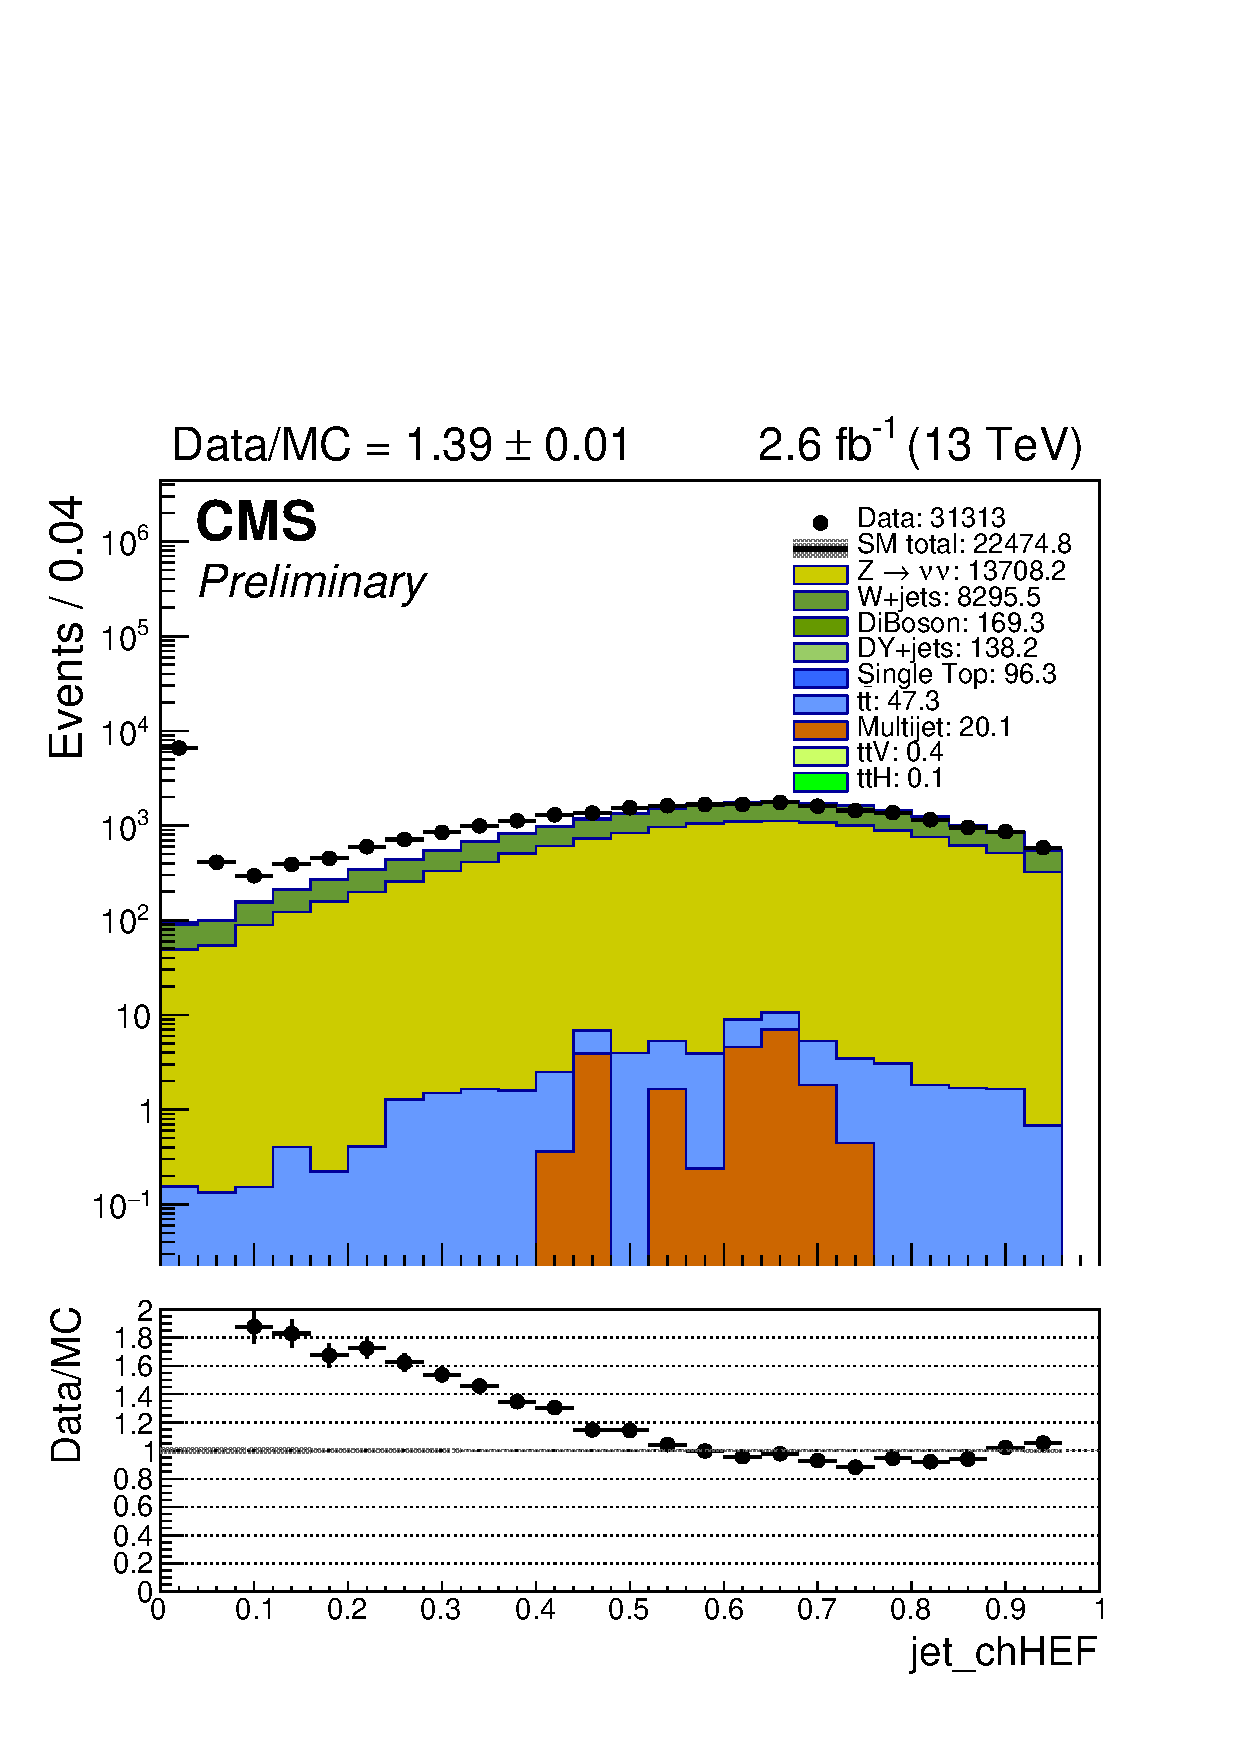
\includegraphics[width=0.32\textwidth]{figs/analysis/jet_chHEF_mono_all_before.pdf}
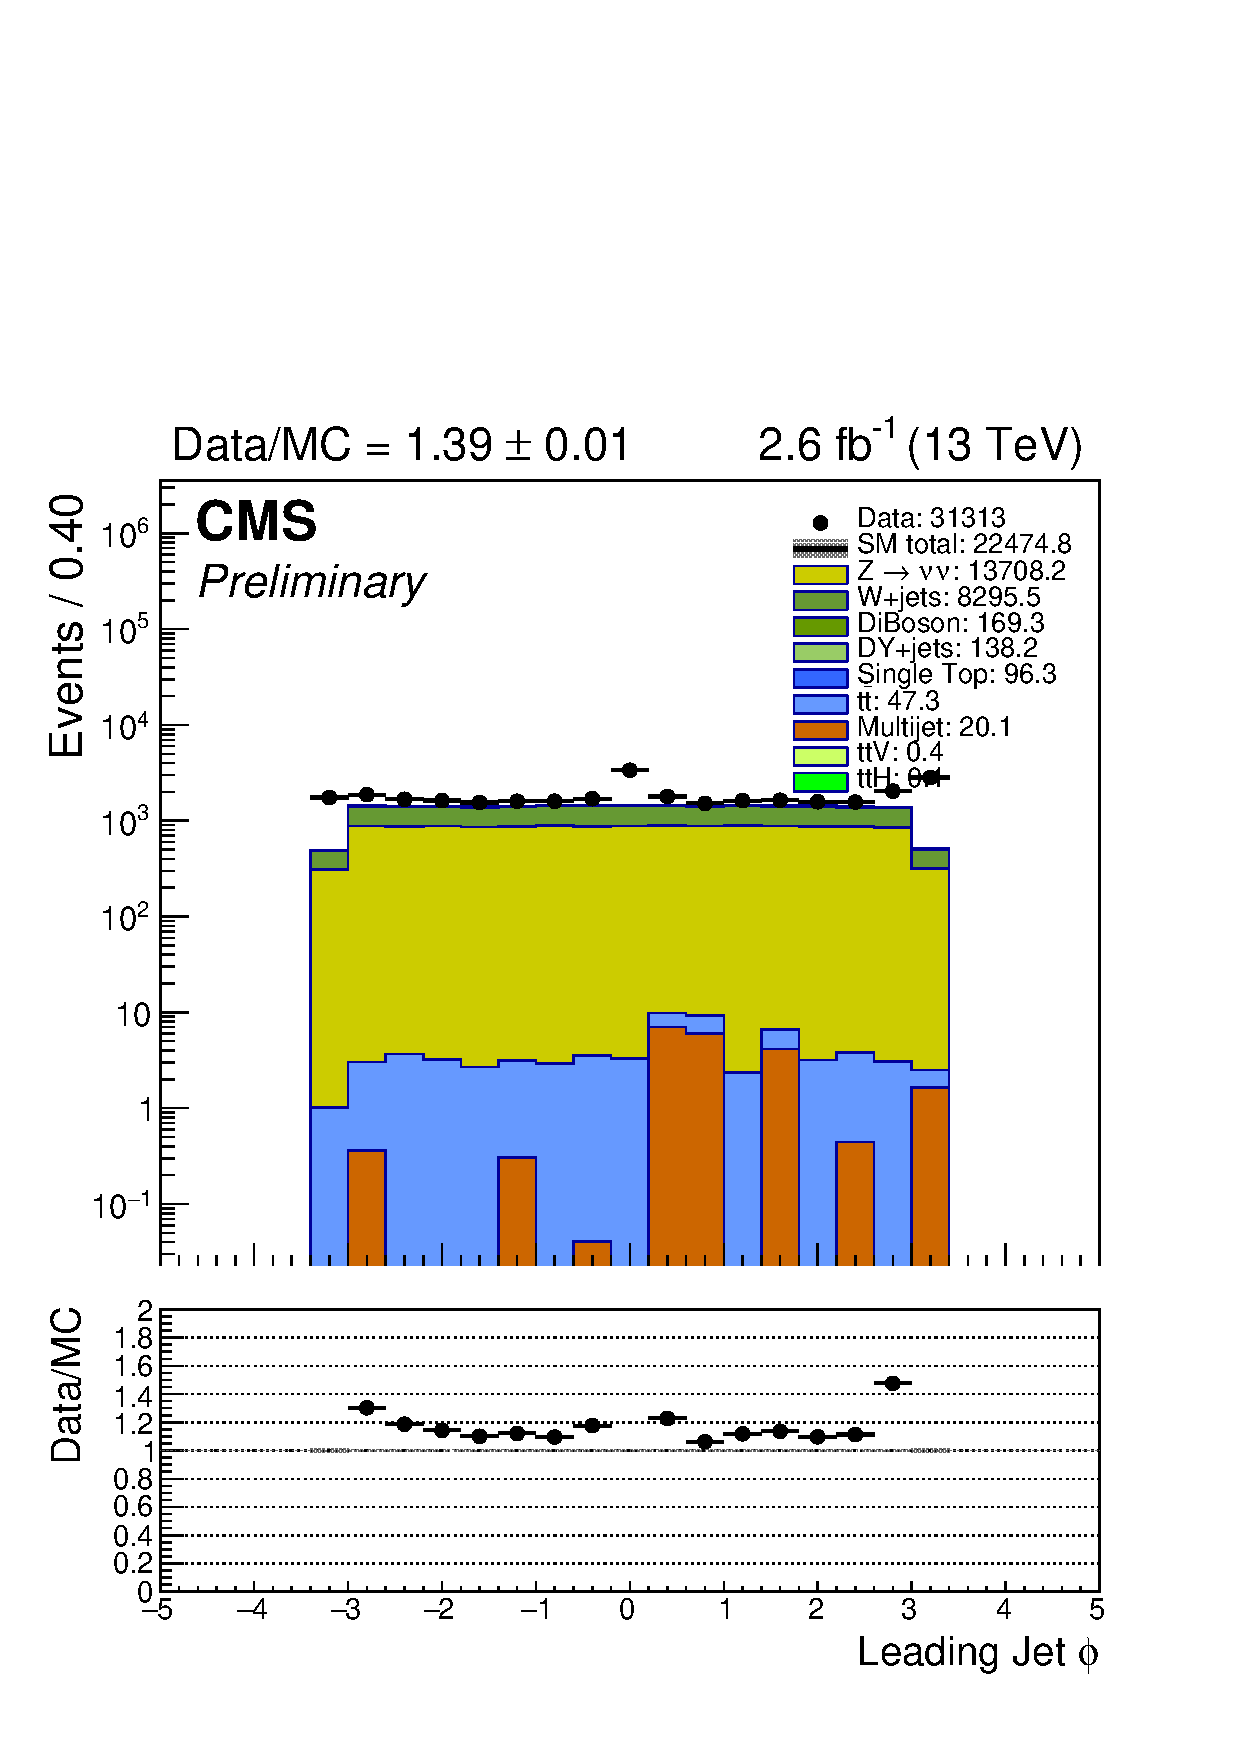
\includegraphics[width=0.32\textwidth]{figs/analysis/jet_phi[0]_mono_all_before.pdf}
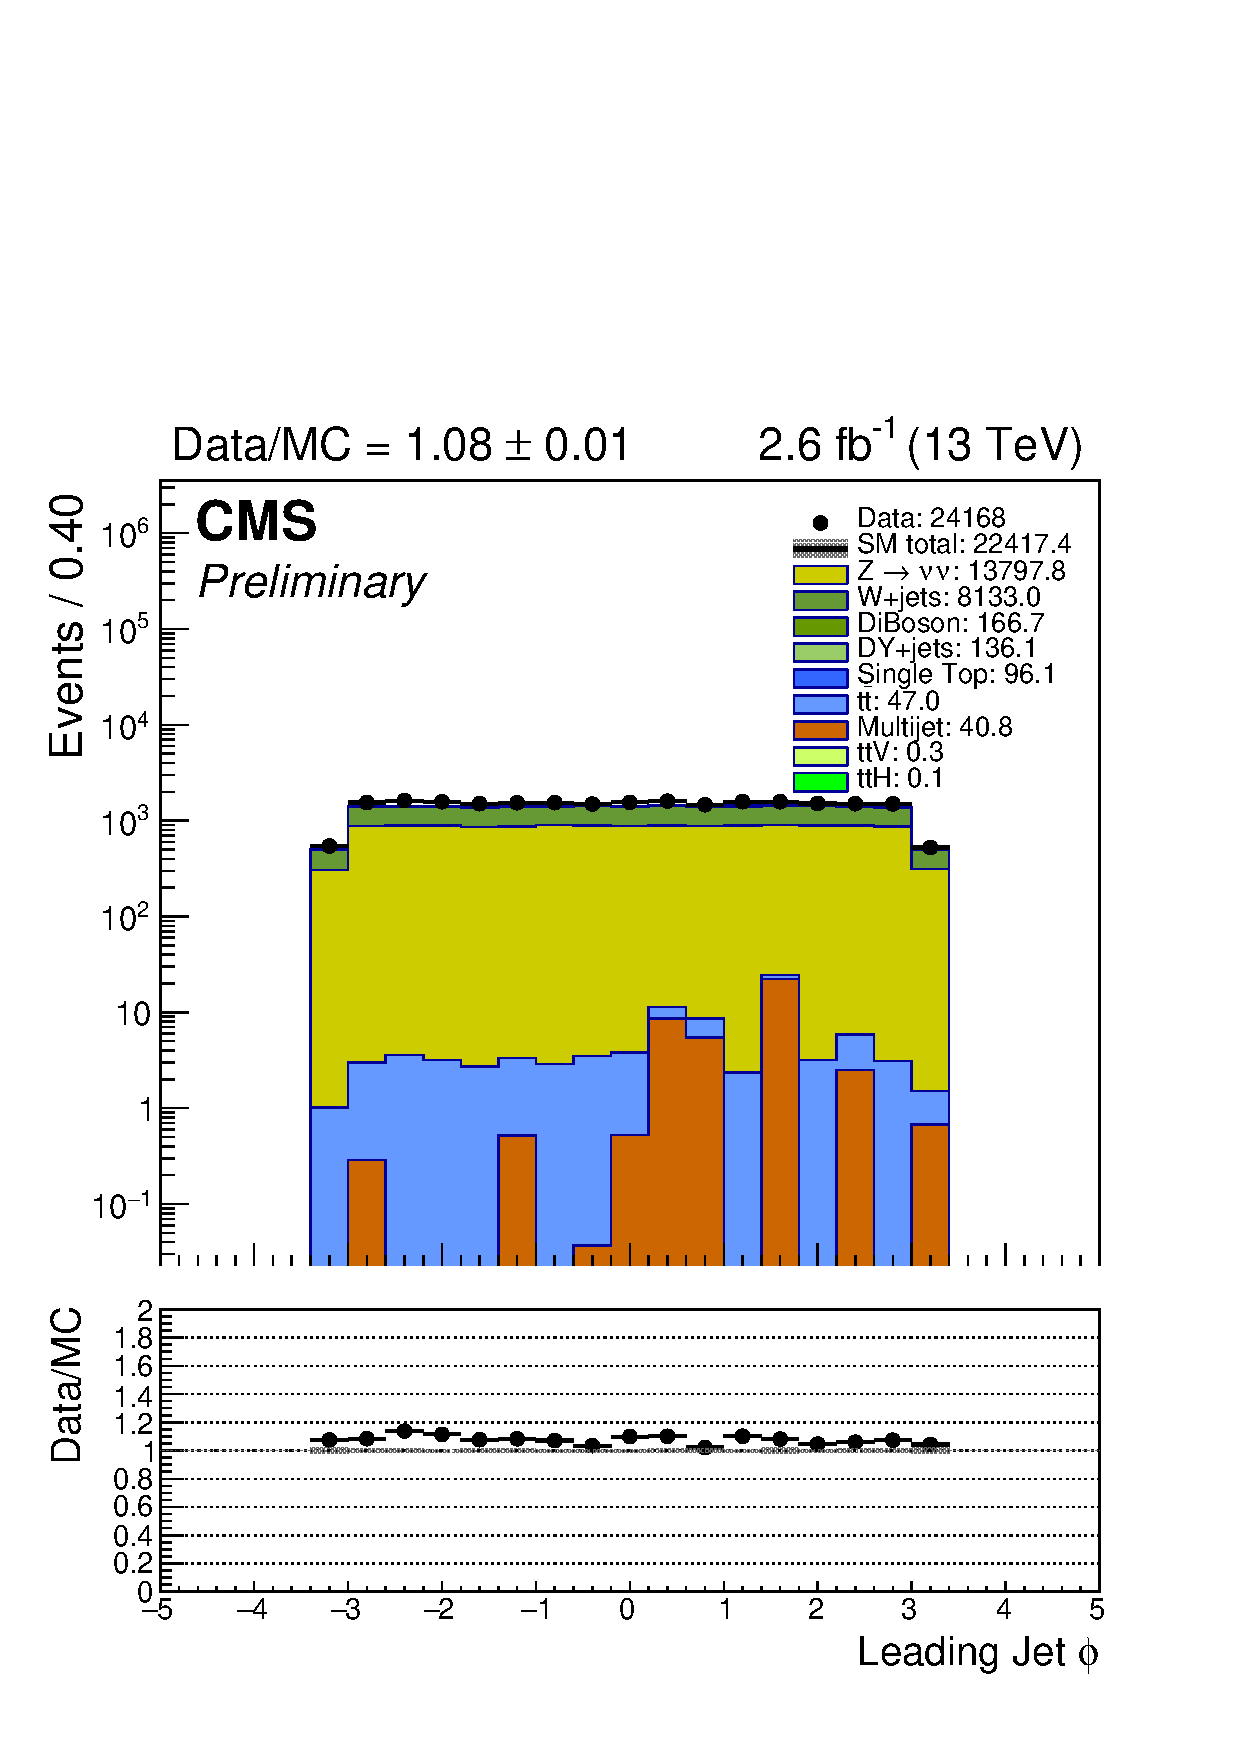
\includegraphics[width=0.32\textwidth]{figs/analysis/jet_phi[0]_mono_all_after.pdf}
\caption{The leading jet's charged hadron energy fraction (Left) and $\phi$ 
direction before (Centre) and after (Right) applying a requirement of 
\chf~$>0.1$. The large excess in data at \chf values close to zero and $\phi = 
0$ and $\pi$ is consistent with beam halo effects, and is effectively 
suppressed by the \chf requirement.}
\label{fig:beamhalo}
\end{center}
\end{figure}

%odd jet veto
As a further safeguard against noise and misreconstruction issues, events that 
contain a jet that fails the identification requirements outlined in 
Sec.~\ref{sec:analysis-physicsobjects} are not considered.

%Forward jet veto here or QCD rejection? both
Finally within the set of baseline selections, events are vetoed if there are 
any jets with pseudorapidity direction \etaabs~$>2.4$. This threshold 
corresponds to the extent of the tracker and hence ensures well reconstructed 
jets and a better resolution of the energy sums. This requirement also has the 
added benefit of rejecting a larger proportion of background, particularly QCD 
processes, compared to signal processes, which tend to have more central 
jets.
%Adam: As most BSM physics scenarios result in the production of particles at a 
%high mass scale, they are more likely to deposit their energy centrally than 
%many of the SM backgrounds. Therefore, this forward jet veto does not 
%significantly effect the signal efficiency for most models. The QCD multijet 
%background consists of many soft scattering events, which typically deposit a 
%significant proportion of energy within the forward region

\section{Standard model backgrounds}
%2-3 pages

%After these requirements, still left with significant SM backgrounds from 
%electroweak and QCD processes.
The baseline selections described in the previous section select events with 
significant hadronic activity and missing energy, as desired. However, a large 
number of standard model events still remain. These include processes (labelled 
electroweak background processes) with `genuine' missing energy in the final 
state due to neutrinos, as well as QCD multijet processes with `fake' missing 
energy in the final state due to jet energy mismeasurements.

Give rough proportions and what regions of njnbht phase space they occupy. 
Branching fractions.

\subsection{Electroweak processes}

The dominant electroweak background process (comprising $\sim$50\% of the 
signal region background events) is the production of a Z boson in 
association with jets, with the Z boson decaying to two neutrinos. This 
background is irreducible as the final state consists of only jets and missing 
energy, just like the SUSY and DM models being searched for.
% Z boson BF to neutrinos.

The second largest background process (making up $\sim$40\% of the total 
background) is the production of a W boson in 
association with jets, with the W boson decaying semi-leptonically to a lepton 
and a neutrino. Such an event may not be vetoed if the lepton is not 
reconstructed or travels in a direction that is outside the acceptance of the 
detector, or is a muon or electron that fails the kinematic, identification, or 
isolation criteria listed in Sec.~\ref{sec:analysis-physicsobjects}. If the 
lepton 
is a tau, it may decay semi-leptonically to a muon or electron that is not 
vetoed for the aforementioned reasons, or it may decay hadronically resulting 
in a jets + \met final state. In the case of a single-prong hadronic decay, the 
tau background is suppressed with a veto on events containing an isolated 
track, as mentioned in Sec.~Selections. The veto on isolated tracks cannot 
capture three-prong decays, however, as the tracks are usually not isolated and 
are instead reconstructed as a jet.
% W branching fractions.
% W --> tau 6%
% 70% single prong

The third largest background process (constituting $\sim$5\% of the signal 
region background) is the production of top quark-antiquark pairs 
(\ttj). This background is characterised by b-jets and a larger number 
of jets in the final state compared to the other two dominant backgrounds.  
Each top quark decays to a bottom quark and W boson, and each W boson can decay 
hadronically or semi-leptonically. The dominant decay mode in the signal region 
is the one in which one of the W bosons decays hadronically and the other 
decays semi-leptonically, resulting in a lepton that is then `lost' in the same 
way as for the \wlj background described previously. The decay mode in which 
both W bosons decay hadronically is negligible because there is no significant 
amount of \met in the final state. The decay mode in which both W bosons decay 
semi-leptonically is also negligible because of the low probability of losing 
both leptons.
% ttbar BRs: 45,45,20% had,semilep,lep

Additional, residual standard model background processes include the production 
of a single top quark (in association with a b quark, light quark, or W boson), 
the production of vector boson pairs (WW, WZ, ZZ), \ttbar production in 
association with a vector boson, \zllj production, and \gj production.
% single top feynman http://inspirehep.net/record/1205888/files/SingleTop.png

\subsection{QCD processes}
%Several OOMs (several, Matt: 7) larger than other backgrounds because of 
%massive xs at hadron collider.
%Different QCD mechanisms (bullet list plus my studies) - detector effects, 
%fake MET, mismeasurement, below threshold, heavy flavour.

% check what QCD xs is and how much larger it is.

At a hadron collider such as the LHC, the dominant/most abundant process is 
that of QCD multijet production, having a cross section that is several 
OOM/seven times [FIXME] larger than other standard model processes. The final 
state consists of two or more jets, and there is no missing energy (except in 
the case of heavy flavour QCD, as discussed below). However, issues with the 
detector or inaccuracies in the reconstruction [FIXME: tails of Gaussian 
resolution] can cause the event to appear 
unbalanced in transverse momentum, thereby introducing fake \met. Although 
these effects are not very common, when coupled with the large QCD production 
cross section, the result is that QCD multijet production remains as the 
largest background even when requiring a reasonable amount of \met such as 
200~GeV. The following is a comprehensive list of the various mechanisms by 
which QCD processes can have a large amount of missing energy. The 
next section will describe a set of variables that are used to identify and 
reject/suppress this type of background.

%see my studies: RA1_QCDMC_161101
% AcceptanceEffect, HeavyFlavour, Mismeasurement (MismeasurementLostJet, 
%SingleMismeasurement, MultipleMismeasurement, HotCellEffect)
\begin{itemize}
	\item Soft jets with transverse momentum \pt~$<40$~GeV are not included in 
	the computation of the jet energy sums, and therefore result in an 
	apparently unbalanced event.
	%contribute to a non-zero met
	The resulting missing jet energy is particularly significant when there are 
	several jets below the \pt threshold. A similar problem can occur when the 
	jets are outside the acceptance of the detector.
	% Inaccurate measurements
	\item Significant over or under-measurements of jets' energies due to the 
	tails of the resolution distribution. This includes the mismeasurement of a 
	single jet in the event, in which case the missing transverse momentum 
	vector is collinear (if the jet's energy is under-measured; or 
	anti-collinear
	if it is over-measured) to the jet's direction, as well as the 
	mismeasurement of two or more jets, in which case the missing momentum is 
	not aligned with any jet. A third effect is when a jet is severely 
	under-measured such that its measured transverse momentum is below the 
	40~GeV threshold. 
	\item Detector effects, such as dead cells and hot cells in the 
	calorimeters, can result in a large amount of fake missing energy. These 
	effects are dealt with by the dedicated \met filters described in 
	Sec.~\ref{analysis-baselineselections}.
	% hot cell: electronics noise
	\item The production of bottom quarks with a subsequent semi-leptonic decay 
	leads to genuine missing energy in the final state due to the resulting 
	neutrino. The lepton and neutrino are typically contained within the jet 
	cone. This means that the lepton is not isolated and so such events are not 
	rejected by the lepton veto. It also means that the missing transverse 
	momentum vector is roughly collinear with the jet. %small azimuthal 
	%separation
\end{itemize}

The dominant mechanism by which QCD processes can pass the baseline selections 
is that due to jet energy mismeasurements ($\sim$70\%), followed by threshold 
effects ($\sim$30\%). The heavy flavour and detector effects are comparatively 
much smaller ($\sim$1\%).
%numbers taken from slide 11 of 160509


\section{QCD background rejection}
%4-5 pages.

It is important to suppress the overwhelming QCD background so that it does not 
swamp any potential signal. This section describes three key variables 
(\alphat, \bdphi, and \mhtmet) that effectively distinguish QCD events from 
events with genuine missing energy. Each variable exploits certain topological 
or kinematical features, and each one targets different sources of missing 
energy of those described in the previous section.

Events in the signal region need to satisfy certain requirements on these 
variables, as will be in outlined in Sec.~\ref{analysis-eventselection}. These 
thresholds are chosen such that the QCD background forms no more than $\sim$1\% 
of the total standard model background in the signal region. This choice is 
motivated by the difficulty in estimating this type of background accurately 
and precisely. The difficulty arises from the lack of precise [FIXME: high 
order?] theoretical calculations on the production cross section and kinematic 
properties. 
In addition, because of the large cross section and computing limitations, the 
number of simulated events is much smaller than that expected by the integrated 
luminosity of $35.9$~\ifb, and so the simulated events have large weights and 
hence large statistical uncertainties.
%necessitates an infeasibly large number of simulated events , which due to 
%computing limitations,  which necessitates.
Therefore, if QCD processes were to form a large part of the total expected 
background this would significantly reduce the sensitivity of the search. A 
small contribution of $\sim$1\%, even with a large uncertainty, has a 
negligible impact on the sensitivity.
%choose cuts such that backgroudn rej is 1\% and signal eff is
%, while maintaining a good acceptance to signal events
%Want to kill it (aim for sub-percent) because very difficult to model in 
%simulation and requires lots of MC stat. Prefer conservative unc on small 
%contribution than trying to estimate large contribution.

%[TODO] If have time make diagrams illustrating alphat and bdphi.

\subsection{The \alphat variable}

The \alphat variable is designed to discriminate between balanced events that 
may contain mismeasurements and unbalanced events containing invisible 
particles~\cite{alpha-variable}. For a dijet event it is defined as:
\begin{equation}
\alpha_\mathrm T = \frac{E_\mathrm{T}^{j_2}}{M_\mathrm{T}}, 
\end{equation} 
where $E_\mathrm{T}^{j_2}$ is the transverse energy of the least energetic jet, 
and $M_\mathrm{T}$ is the transverse mass of the dijet system, which is given 
in general for a number of jets by:
% define ET=Esintheta?
\begin{equation}
M_\mathrm{T} = \sqrt{\left(\sum_{i}E_{\mathrm T}^{j_i}\right)^2 - 
\left|\sum_{i}\bm{p}_\mathrm{T}^{j_i}\right|^2},
\end{equation}
where $E_{\mathrm T}^{j_i}$ is the transverse energy of the $i^\mathrm{th}$ 
most energetic jet, and 
$\bm{p}_\mathrm{T}^{j_i} = (p_x^{j_i}, p_y^{j_i})$ is its 
transverse momentum vector, $p_x^{j_i}$ and $p_y^{j_i}$ being the $x$ and $y$ 
components, respectively. [FIXME] already defined in MHT definition?

To illustrate how the \alphat variable works, one can assume the mass of the 
jets to be much smaller than their momenta (so that $E_\mathrm T \approx 
p_\mathrm T$, which is a good approximation for jets produced at the LHC), and 
rewrite $M_\mathrm T$ in terms of the 
azimuthal angle $\Delta\phi(j_1,j_2)$ between the two jets such that:
\begin{equation}
\alpha_\mathrm T \approx \frac{E_\mathrm{T}^{j_2}}{\sqrt{2E_{\mathrm 
T}^{j_1}E_{\mathrm T}^{j_2}(1-\mathrm{cos}\Delta\phi(j_1,j_2))}}.
\end{equation}
If the jets have equal and opposite transverse momenta such as in a QCD dijet 
event, then the azimuthal angle between them is $\pi$, their transverse 
energies are the same, and the value of \alphat is exactly $0.5$. If one of the 
jets' energies is mismeasured, then $E_\mathrm{T}^{j_2} < E_\mathrm{T}^{j_1}$ 
and \alphat takes values less than $0.5$. In an event where the jets are 
recoiling against a system of invisible particles, the angle between them is 
smaller than $\pi$ and the value of \alphat is generally larger than $0.5$.

For events with more than two jets in the final state, the jets can be grouped 
into two \textit{pseudo jets} such that the difference in transverse energy 
$\Delta E_\mathrm T$ between the two pseudo jets is minimised, where the 
transverse energy of a pseudo jet is computed via the vector sum of the 
transverse energies of the constituent jets. This is done so that the resulting 
pseudo dijet system is as close to a balanced event as possible. Since $\Delta 
E_\mathrm T = E_\mathrm{T}^{j_1} - E_\mathrm{T}^{j_2}$ and 
$|\Sigma_i\bm{p}_\mathrm{T}^{j_i}| = \mht$, the general form of the \alphat 
variable can be defined as:
\begin{equation}
\alpha_T=\frac{\Sigma_i E_\mathrm{T}^{j_i}-\Delta 
E_\mathrm{T}}{2\sqrt{(\Sigma_i E_\mathrm{T}^{j_i})^2-\cancel{H}_\mathrm{T}^2}}.
\end{equation}

For balanced QCD events with no missing energy, $\Delta E_\mathrm T = \mht = 0$ 
and $\alphat = 0.5$. If a jet in such an event is mismeasured, then $\Delta 
E_\mathrm T \approx \mht$ and $\alphat < 0.5$. For events with genuine missing 
energy, $\mht > 0$ and $\Delta E_\mathrm T = 0$, resulting in $\alphat > 0.5$.

The discriminating power of the \alphat variable is shown in 
Fig.~\ref{fig:alphat}. Multijet QCD events are the dominant process in the 
region of $\alphat \leq 0.5$, while processes with genuine missing energy 
occupy the region of $\alphat > 0.5$. It is possible for QCD events to have 
values of \alphat slightly larger than $0.5$ if there is a severe 
mismeasurement or there are several jets below the \pt threshold.

% Does it deal with multiple mismeasurements?

% remember my plot of alphat vs mismeasurement - starts at 0.5, falls, then 
%shoots up for large mismeasurement

%matt/AN: The αT distribution becomes more sharply peaked with increasing HT in 
%the event as mismeasurements are larger for lower jet pT

\begin{figure}[t!]
\begin{center}
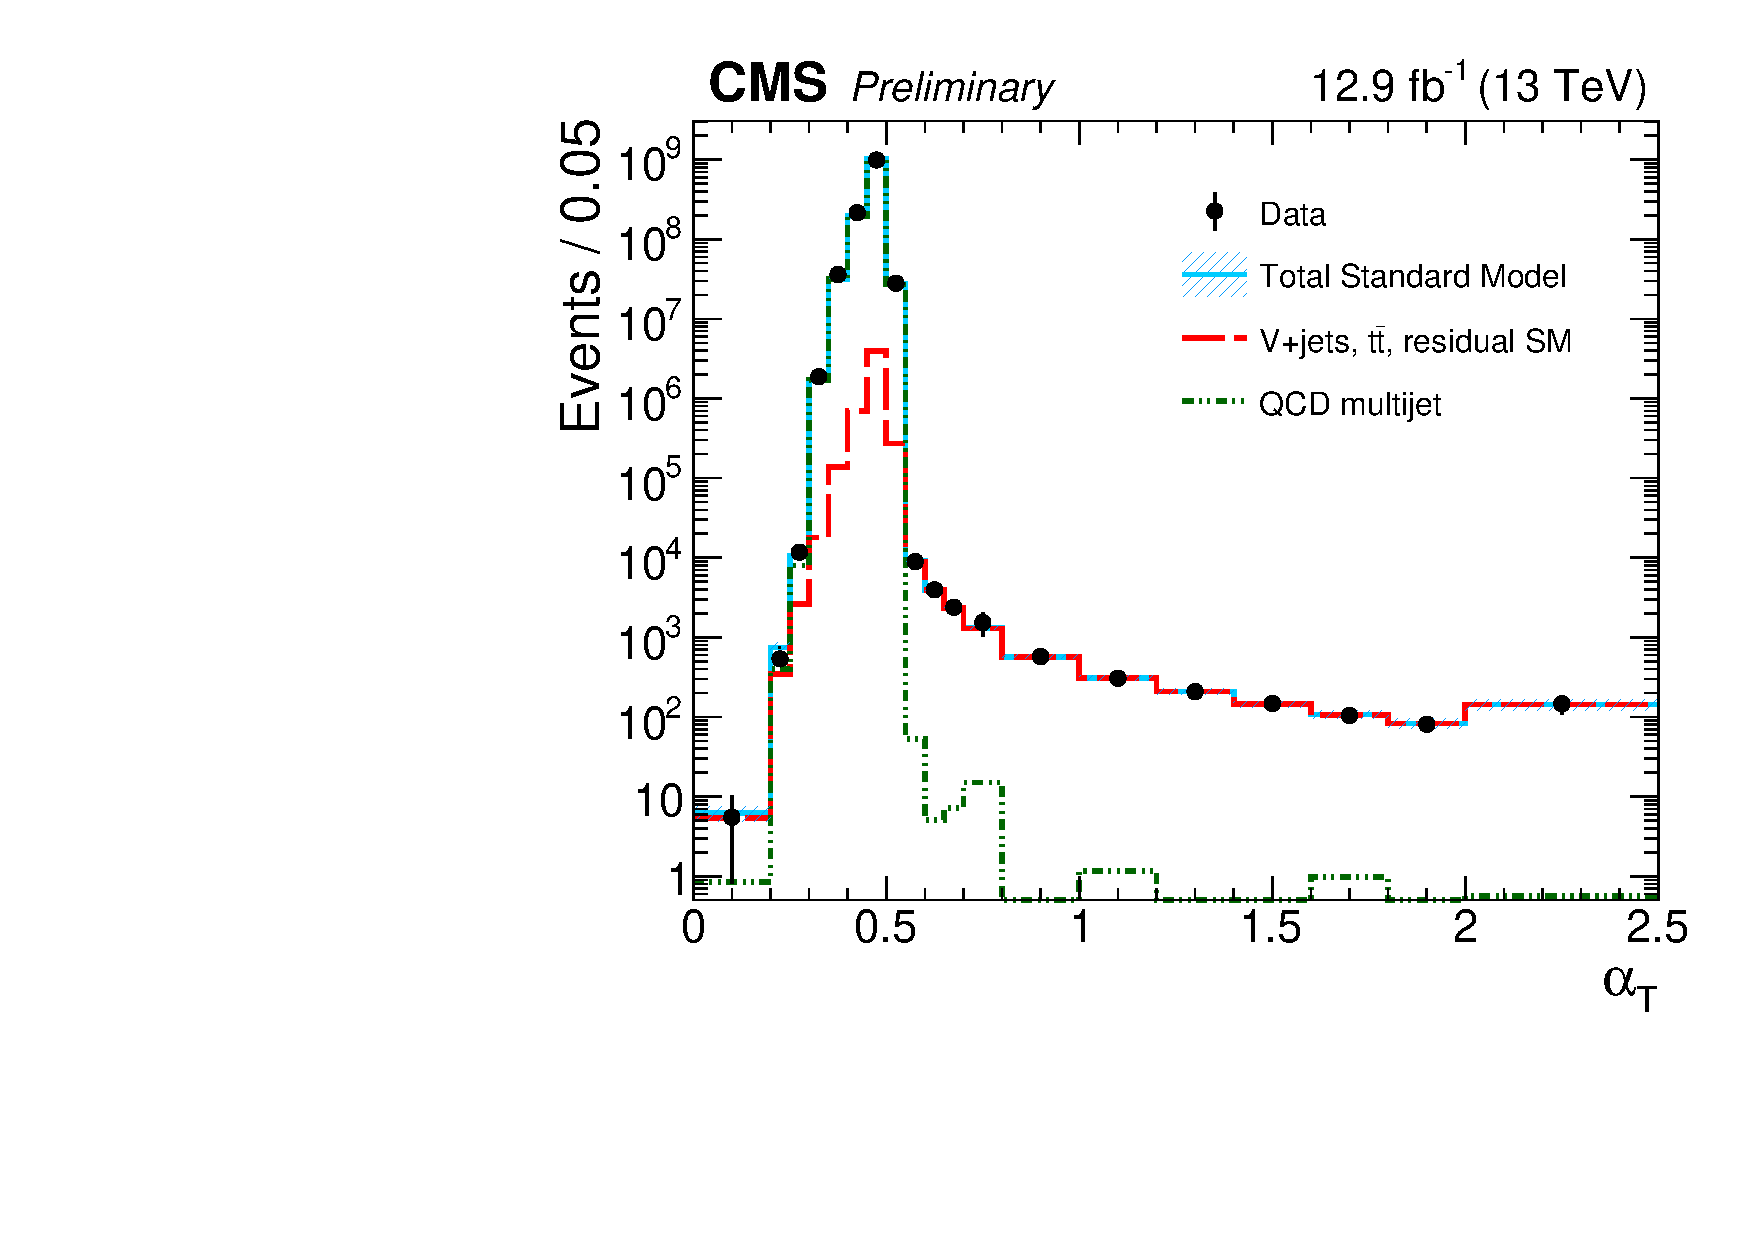
\includegraphics[width=0.7\linewidth]{figs/analysis/propaganda_alphat}
\caption{The distribution of the \alphat variable in data and simulation for 
events satisfying the signal region selections 
(Sec.~\ref{analysis-eventselection}) except the \alphat requirement. The 
ability of the variable to effectively discriminate between QCD processes and 
processes with genuine missing energy is evidenced by the sharp edge at $0.5$. 
[FIXME: actually, presel left full sel right]}
\label{fig:alphat}
\end{center}
\end{figure}

\subsection{The \bdphi variable}

The \bdphi variable also provides powerful discrimination between events with 
fake missing energy and genuine missing energy.
% note if mht=0 for qcd, dphi is undefined, whereas alphat=0.5 and captures it
First it is instructive to consider the \dphimin variable, which is the minimum 
(over all jets in the event above the \pt threshold) azimuthal angle between a 
jet and the missing transverse jet energy vector:
\begin{equation}
\Delta\phi_{\mathrm{min}} = \mathrm{min}~\Delta\phi\left(\bm{p}_{\mathrm 
T}^{j_i},\bm{\cancel{H}_\mathrm{T}}\right).
\end{equation}
If a jet's energy in the final state is under-measured, the missing energy 
vector is collinear with the jet direction, and so \dphimin is zero, whereas 
for processes in which the jets are recoiling against genuine missing energy, 
the value of \dphimin is non-zero.

However, if a jet's energy is over-measured, the missing energy vector points 
in the opposite direction to the jet and so \dphimin is not necessarily zero. 
This limitation can be overcome by comparing the jet's direction with the 
missing energy vector that does not consider the jet in the vector sum, 
$\vec{\mht}^{j_i} = \vec{\mht} + \vec{p}_{\mathrm T}^{j_i}$. This is the 
definition of the 
\bdphi variable:
\begin{equation}
\Delta\phi^{*}_{\mathrm{min}} = \mathrm{min}~\Delta\phi\left(\bm{p}_{\mathrm 
	T}^{j_i},\bm{\cancel{H}}_\mathrm{T}^{j_i}\right).
\end{equation}

The discriminating power of the \bdphi variable is shown in 
Fig.~\ref{fig:bdphi}. Multijet QCD events have values of \bdphi close to 0, 
with the distribution falling sharply beyond this, 
whereas processes containing genuine missing energy exhibit a longer tail up to 
values of $\pi$ radians.

The \bdphi variable is effective at capturing QCD events that contain a single 
mismeasurement or a neutrino produced by a heavy quark decay that is collinear 
with a jet. It is less effective if a jet is severely mismeasured such 
that it's \pt is below threshold, or if there are two or more mismeasured jets. 
Both of these cases result in missing momentum that is not necessarily 
collinear with any jet.

%captures single mismeasurements and heavy flavour
%captures both under and over measurements
%doesn't capture severe mismeasurements (would need to lower threshold)

\begin{figure}[t!]
\begin{center}
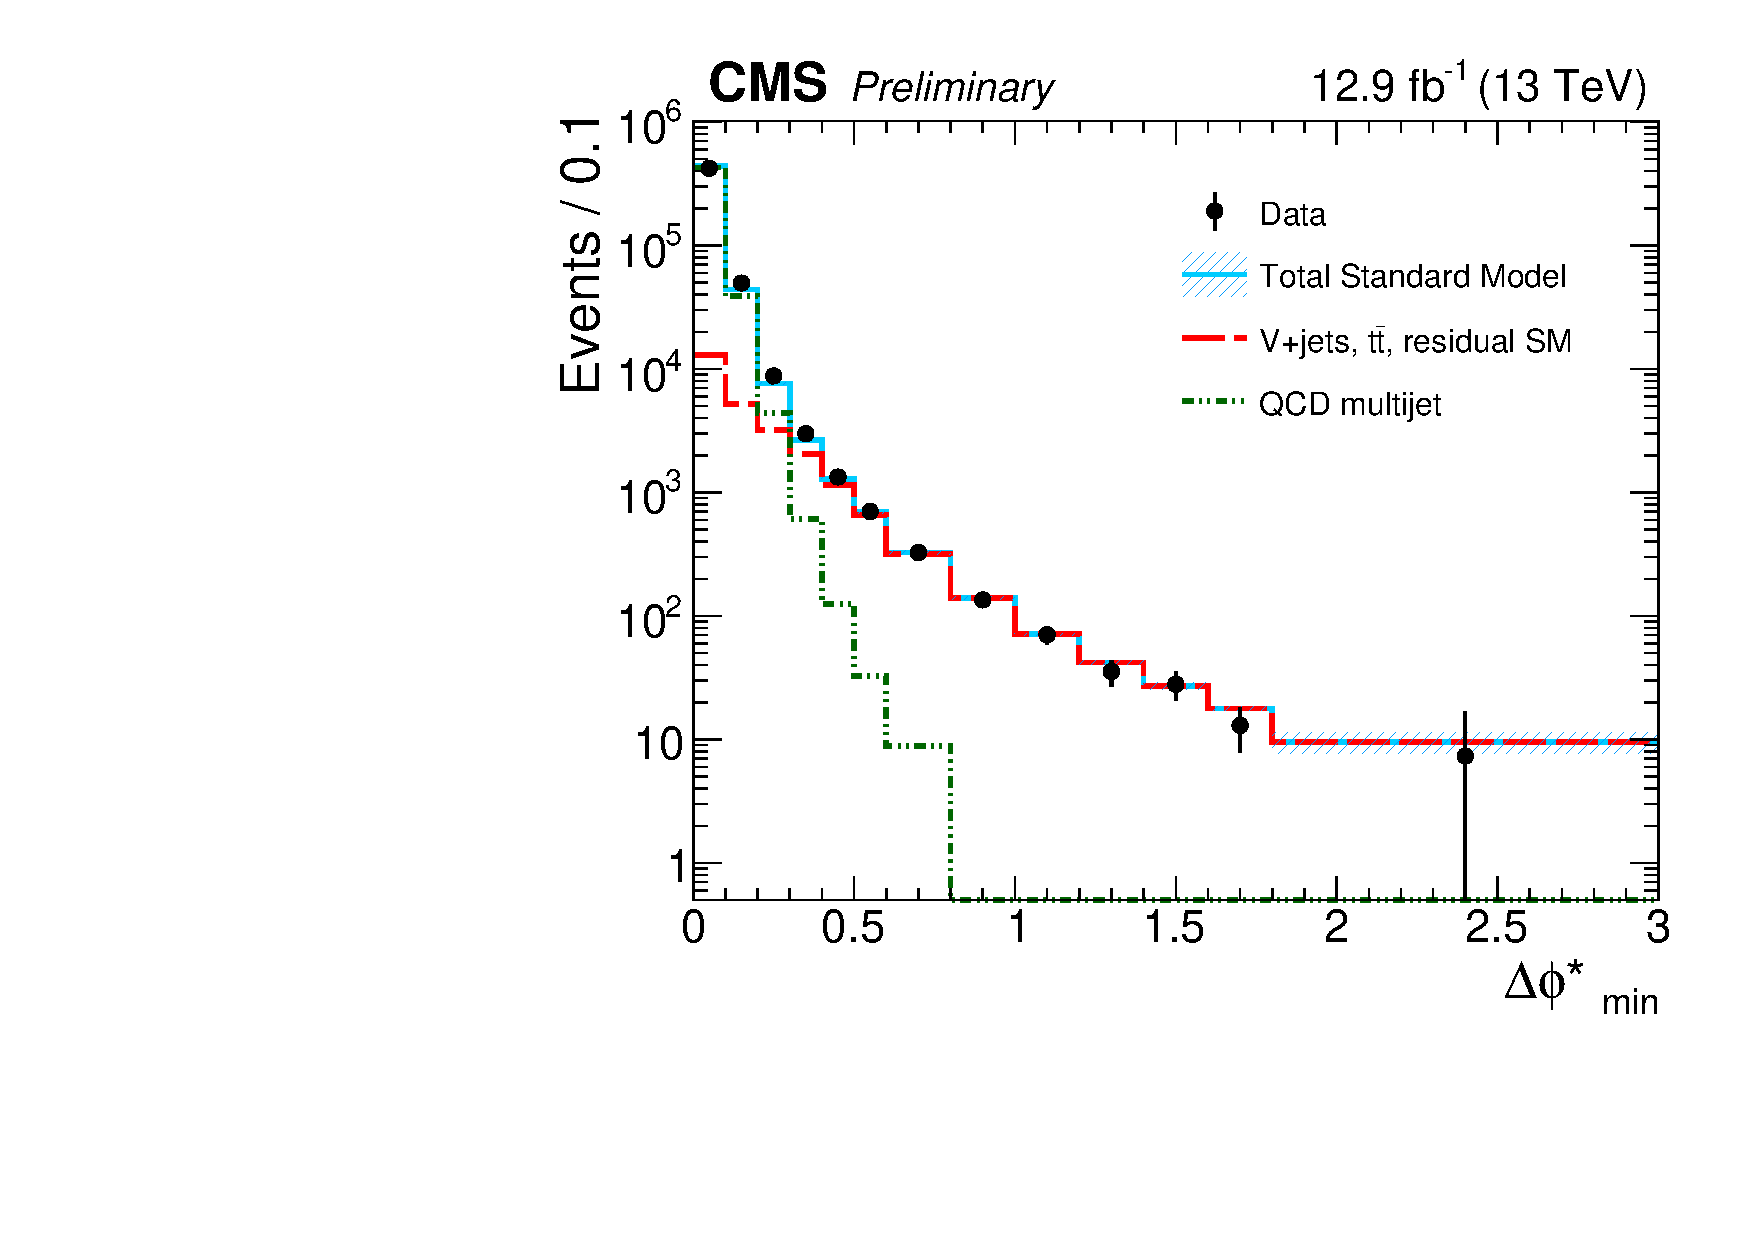
\includegraphics[width=0.7\linewidth]{figs/analysis/propaganda_bdphi}
\caption{The distribution of the \bdphi variable in data and simulation for 
events satisfying the signal region selections 
(Sec.~\ref{analysis-eventselection}) except the \bdphi requirement. The ability 
of the variable to effectively discriminate between QCD processes and processes 
with genuine missing energy is evidenced by the cluster of QCD events close to 
0, while processes with genuine \met take on larger values up to $\pi$ radians.}
\label{fig:bdphi}
\end{center}
\end{figure}

\subsection{The \mhtmet variable}

As mentioned previously, the \alphat and \bdphi variables are not as effective 
at identifying QCD events in which there are several jets with transverse 
momentum below the 40~GeV threshold. In such events, the value of \mht is 
biased to larger values. The \met variable, however, is computed using all PF 
objects in the event satisfying a much lower threshold (10~GeV for jets) 
[FIXME: is it actually 10?] and so is less susceptible to this bias and remains 
closer to zero. One can compare the values of \mht and \met to identify these 
events -- the ratio of \mhtmet tends to be significantly larger than 1 for such 
events. 

For processes with genuine missing energy, on the other hand, the ratio 
generally remains close to unity as the increase in missing energy due to 
threshold effects is proportionally smaller with respect to the true missing 
energy which is already relatively large. The distribution of the \mhtmet 
ratio is shown in Fig.~\ref{fig:mhtmet} and demonstrates the difference between 
the two types of backgrounds. Multijet QCD processes tend to populate the 
region of \mhtmet$>1.25$.

\begin{figure}[t!]
\begin{center}
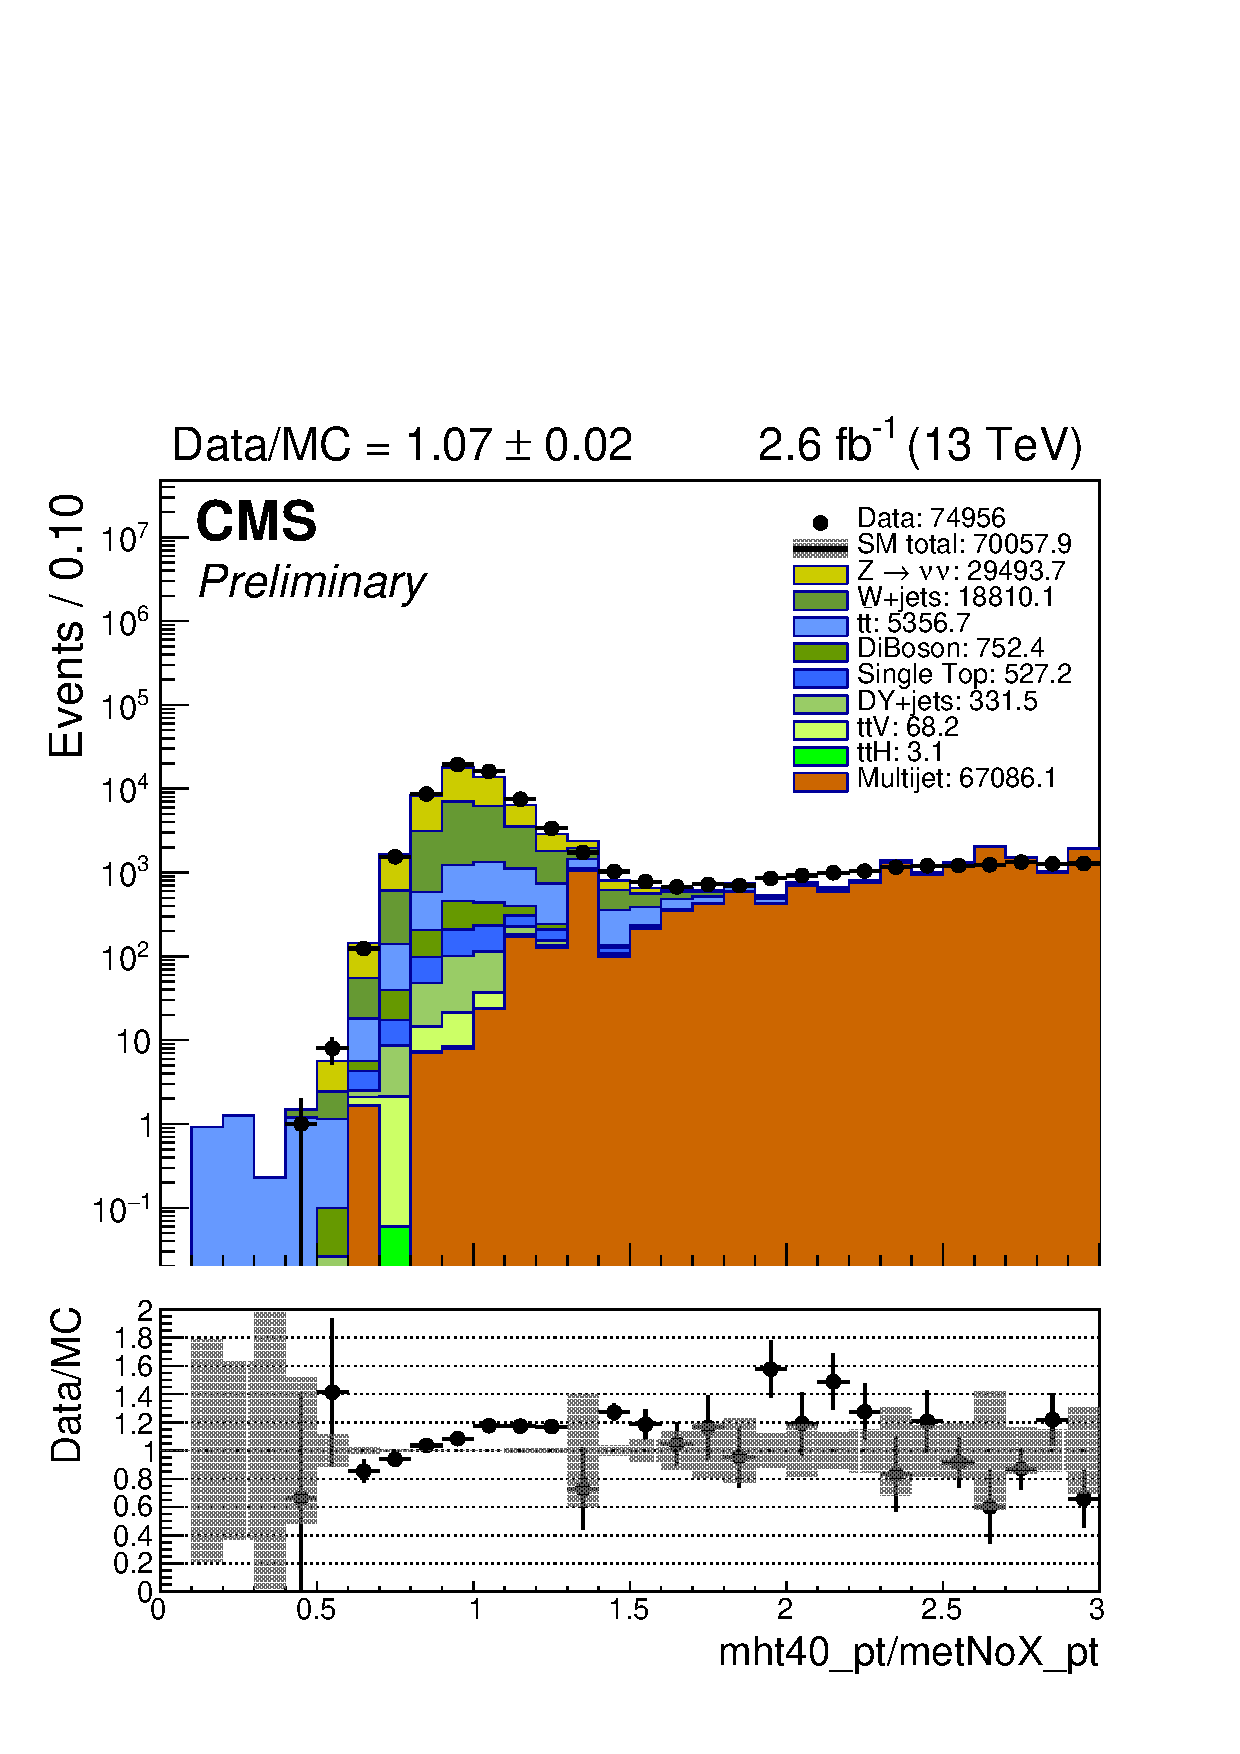
\includegraphics[width=0.7\linewidth]{figs/analysis/mhtmet}
\caption{The distribution of the \mhtmet ratio in data and simulation for 
events satisfying the signal region selections 
(Sec.~\ref{analysis-eventselection}) except the \mhtmet requirement. The 
ability of the variable to effectively discriminate between QCD processes and 
processes with genuine missing energy is evidenced by the population of QCD 
events above $1.25$, while processes with genuine \met have values more 
consistent with 1. [FIXME: remove ratio plot and fix axis label? Update to 
36fb]}
\label{fig:mhtmet}
\end{center}
\end{figure}




\textbf{FIXME
multiple mismeasurements is kinda irreducible.
This and severe mismeasurements below threshold are the two dominant mechanisms 
left in the SR after these qcd killing selections.
Nevertheless still sub-percent.
Begs question whether sidebands are suitable. Have an answer or don't mention 
the mechanisms.}




\section{Event selection}
\label{sec:analysis-eventselection}
%2-3 pages

After the baseline selections outlined in 
Sec.~\ref{sec:analysis-baselineselections}, additional selections are applied 
in order to suppress the QCD background in the signal region and enrich the 
control regions in the relevant standard model processes that need to be 
estimated. These are described in this section and are summarised, along with 
the baseline selections described in 
Sec.~\ref{sec:analysis-baselineselections}, in Tab.~\ref{tab:selections}.

%Big summary table of all selections/regions/objects (see paper). Or have a 
%smaller table within each section.
%define mono sym asym somewhere - sec. categorisation?

% PRIMARY VERTEX SELECTION?
\begingroup
\renewcommand*{\arraystretch}{1.4}
\begin{table}[h!]
\label{tab:selections}
\centering
\footnotesize
\begin{tabular}{ll}
\hline
%\multicolumn{2}{l}{\bf Baseline event selection}
\textbf{Baseline selection} & \\
All-jet final state & At least one jet; no muons, electrons, photons or 
isolated tracks \\
\met quality & No spurious \met due to instrumental effects or beam halo \\
Jet energy and sums & $p_{\mathrm T}^{j_1}>100$~GeV, $\scalht>200$~GeV, 
$\mht>200$~GeV \\
Jets outside acceptance & $\mhtmet<1.25$; no jets with $\etaabs>2.4$ \\
Jet quality & No jets that fail identification criteria \\
\hline
\textbf{Signal region} & Baseline selection + \\
\alphat ($>$) (\scalht GeV range) & 0.65 (200-250), 0.60 (250-300), 0.55 
(300-350), 0.53 (350-400), 0.52 (400-900) \\%($\njet \geq 2$) \\
\bdphi & $\bdphi>0.5$ \\
\hline
\textbf{Control regions} & Baseline selection + \\
\mj & One muon; $\mathrm{min}~\Delta R(\mu,j_i) > 0.5$; $30 < 
M_{\mathrm{T}}(\mu,\met) < 125$~GeV \\
\mmj & Two muons opp.~charge; $\mathrm{min}~\Delta R(\mu_{1,2},j_i) > 0.5$; 
$|M(\mu_1,\mu_2) - m_\mathrm{Z}| < 25$~GeV \\
Hadronic & Signal region sidebands $1.25<\mhtmet<3.0$ and/or $0.2<\bdphi<0.5$ \\
\hline
\end{tabular}
\caption{Summary of selections as part of the definition of the signal and 
control regions.} %topcaption
\end{table}
\endgroup

\subsection{Signal region}

The baseline selections in the signal region are chosen to ensure a hadronic 
final state with significant energy and missing momentum that is characteristic 
of the DM and SUSY models that are sought. As a reminder, these include minimum 
requirements on \scalht and \mht, and event vetoes on non-hadronic objects and 
forward jets as well as spurious \met sources. However, a large number of QCD
events remain that contain fake missing energy (or missing energy from heavy 
quark decays). This background is suppressed to a very small level 
($\lessapprox$1\% of the total standard model background) by imposing certain 
requirements on the QCD-discriminating variables \alphat, \bdphi, and \mhtmet 
described in the previous section.

An \scalht-dependent \alphat requirement is used for multijet events, as 
summarised 
in Tab.~\ref{tab:alphatcuts}. For events containing only one jet above 40~GeV, 
\alphat is undefined and no requirement is imposed. The \alphat threshold is as 
high as $0.65$ for 
events with $200<\scalht<250$~GeV, and is reduced with increasing \scalht down 
to $0.52$ for events with $400<\scalht<900$~GeV, while no requirement at all is 
made for $\scalht>900$~GeV. The thresholds are a decreasing function of \scalht 
because the expected number of QCD events falls quickly with increasing 
\scalht. The thresholds are also chosen to ensure that events are triggered 
with full efficiency, as the \alphat trigger thresholds have been chosen to 
provide a reasonable trigger rate. The trigger strategy will be discussed in 
Sec.~\ref{sec:analysis-trigger}.

\begin{table}[h!]
\centering
%\footnotesize
\begin{tabular}{l|cccccc}
\hline
\scalht (GeV) & 200-250 & 250-300 & 300-350 & 350-400 & 400-900 & $>$900  \\
\hline      
\alphat requirement ($>$) & 0.65 & 0.60 & 0.55 & 0.53 & 0.52 & 0 \\
\hline
\end{tabular}
\caption{The \alphat thresholds as a function of \scalht for events containing 
at least two jets. No requirement is made on events containing only one jet.}
\label{tab:alphatcuts}
\end{table}

Any QCD background events not captured by the \alphat selection, in particular 
events with $\scalht>900$~GeV or with only one jet for which there is no 
\alphat requirement, are suppressed by a requirement on \bdphi. The threshold 
is chosen to be $\bdphi>0.5$~radians for all events, regardless of \scalht and 
the 
number of jets. For monojet events, \bdphi is undefined when using only jets 
with $\pt>40$~GeV, and is instead computed using jets that satisfy a lower 
threshold of $\pt>25$~GeV. If there are no jets with $25<\pt<40$~GeV, \bdphi 
remains undefined and no requirement is made on monojet events. The \alphat 
variable could also be defined similarly using jets of lower \pt, but QCD 
events are produced with at least two jets, so QCD monojet events (which must 
result from a severe mismeasurement) form a relatively smaller background and 
these are effectively suppressed by the \bdphi requirement alone.

Finally, in order to suppress the fake \met QCD background due to several jets 
with a transverse momentum below the 40~GeV threshold, a requirement is made on 
the \mhtmet ratio of $\mhtmet < 1.25$.

\subsection{Control regions}
\label{sec:analysis-eventselection-cr}
Each control region is used to estimate a particular standard model background 
process. The estimation methods will be discussed in 
Secs.~\ref{sec:analysis-estimation-ewk}~and~\ref{sec:analysis-estimation-qcd}.
The selections in the control regions are chosen so that they are enriched in 
the background processes that each is designed to estimate, while remaining 
kinematically as similar as possible to the signal region. 
% similar in phase space
For this reason, the 
selections are the same as in the signal region except for the inversion of 
certain requirements and additional purity criteria, as described in the 
following subsections.

In the case of the two muon control regions, the muons are not included in the 
computation of \met (and similarly all jet-based variables) in order to mimic 
the missing energy due to the neutrinos or lost lepton.
% define metnomu = met + pt(muon) if necessary but don't think so
The control regions are also orthogonal to the signal 
region (an event cannot occupy both regions, by construction) and are expected 
to contain very little signal. In any case, any potential signal contamination 
in the control regions is accounted for in the statistical model 
(Sec.~\ref{sec:analysis-likelihood}).

%Enriched in background they want to estimate. similar to SR but No overlap 
%with SR events. 
%Ignored lepton in sums to mimic/proxy the SR. 
%Exactly the same cuts as SR except for inversion of muon veto to selection, 
%plus some other differences described in the following.
%devoid of signal (although account for signal contam)

\textbf{FIXME: Have transverse mass and invariant mass been or need to be 
defined?}

\subsubsection{\mj control region}

The \mj control region is used to estimate the \wlj and \ttbar backgrounds 
(plus the residual backgrounds).
The selections are chosen to identify W bosons, originating from such 
processes, decaying to a muon and a neutrino. 

The muon veto of the signal 
region is inverted and instead exactly one muon (as defined in 
Sec.~\ref{sec:analysis-physicsobjects}) is required. The muon is required to be 
separated from the closest jet by $\Delta R(\mu,\mathrm{jet}) > 0.5$ in order 
to select isolated muons from prompt W decays rather than from QCD decays.

To 
improve the purity in W bosons, the transverse mass of the muon and missing 
transverse energy (which 
is a proxy for the neutrino) is required to be compatible with the W mass with 
$30 < M_{\mathrm{T}}(\mu,\met) < 125$~GeV. The transverse mass must be used 
rather than the invariant mass as the 
z-component of the missing momentum is unknown [FIXME: not sure if this last 
sentence is needed or is already obvious/mentioned previously]. 

All of these 
criteria are effective at selecting a pure sample of \wlj and \ttbar events 
with minimal QCD contamination, and hence no requirements on \alphat or \bdphi 
are made in this control region. This has the benefit of significantly 
increasing the number of events in the control region, which decreases the 
statistical uncertainties associated with the corresponding background 
estimations. Any potential issues in the background estimation arising from 
different \alphat and \bdphi selections are accounted for as a systematic 
uncertainty (see Sec.~\ref{sec:analysis-closuretests}).

\subsubsection{\mmj control region}

The \mmj control region is used to estimate the main irreducible \znnj 
background. The selections are chosen to identify Z bosons decaying to two 
muons. The muon veto of the signal region is again inverted and instead exactly 
two muons, of opposite charge, are required. Each muon is required to be 
separated in $\Delta R$ from jets by the same amount as in the \mj control 
region. In order to improve the purity in Z bosons, the invariant mass of the 
dimuon system is required to be compatible with the mass of the Z boson, with 
$|M(\mu_1,\mu_2) - m_\mathrm{Z}| < 25$~GeV. Similarly to the \mj control 
region, no requirements on \alphat and \bdphi are needed.

% Matt: Electron control regions can provide complementary statistical power to 
%the muon control regions. However, they are not used in the αT analysis due to 
%the significant increase in the rate of fakes from QCD multijet processes 
%compared to the muon control regions.

%\subsubsection{\gj control region}
%used in validation of nb, MHT?
%probably leave out
%TODO

\subsubsection{Hadronic control regions}

Three hadronic control regions are used in the estimation of the small QCD 
background remaining after the full set of selections have been applied. These 
control regions consist of the exact same selections as the signal region, 
except that the \bdphi and \mhtmet requirements are inverted, both individually 
and in conjunction, providing three control regions or ``sidebands'' that are 
enriched in QCD processes. The sidebands are capped such that 
$0.2<\bdphi<0.5$~rad and $1.25<\mhtmet<3.0$. The lower bound on the \bdphi 
sideband and upper bound on the \mhtmet sideband are imposed because [FIXME] 
modelling not right or what? ah trigger?

\subsubsection{\mj and \mmj \mht sidebands}
\textbf{TODO: also two MHT sidebands for sideband corrs.}

\section{Event categorisation}
\label{sec:analysis-binning}
%2-3 pages.
%See AN and paper.

%intro to purpose of binning. to be inclusive to wide range of models; 
%background and signal occupy different regions of parameter space
Events are categorised, or binned, according to four variables. This is done to 
improve the discrimination between signal and background processes, which tend 
to populate different regions of this four-parameter space. Moreover, different 
SUSY and DM processes occupy different regions depending on the particular 
production mode and final state considered. The four variables are the number 
of jets \njet, the number of b-tagged jets \nb, the total jet energy \scalht, 
and the missing transverse jet energy \mht. The binning scheme and motivation 
for each discriminating variable are described in this section.

The control regions are binned identically to the signal region, with some 
exceptions in the \mht and \nb dimensions that will be explained in this 
section. This is done to ensure that the backgrounds are 
estimated (as described in Sec.~\ref{sec:analysis-estimation-ewk}) using events 
in the control regions of similar kinematic and topological properties. Any 
estimations that are not made between equivalent bins, or are made directly 
according to simulation, are assigned an additional systematic uncertainty.

A summary of the bins used in the signal region is provided in 
Tab.~\ref{tab:binning}.
In total, there are 254 bins in the signal region [FIXME: this is aggregated], 
198 in the \mj control 
region, and 122 in the \mmj control region.
%total bins = 254 + 198 + 122 = 574

The hadronic control regions are categorised slightly differently, with coarser 
bins. These regions do not form part of the overall statistical model used to 
derive limits or significances, and instead are used to estimate the QCD 
background separately. This will be discussed in 
Sec.~\ref{sec:analysis-estimation-qcd}.

%Table of bins. (like table 16 in AN)
\begin{table}[h!]
\label{tab:binning}
\centering
\footnotesize
\begin{tabular}{r|r|ccccc}
\hline
\njet & \nb & \multicolumn{5}{c}{\scalht (GeV)} \\
%\hline
%& & \shortstack[c]{200-250, 250-300,\\300-350, 350-400} & 400-500, 500-600 & 
%600-750, 750-900 & 900-1050, 1050-1200 & $>$1200 \\
& & \shortstack[c]{200-250, 250-300,\\300-350, 350-400} & 
\shortstack[c]{400-500,\\500-600} & \shortstack[c]{600-750,\\750-900} & 
\shortstack[c]{900-1050,\\1050-1200} & $>$1200 \\
\hline
       1 &      0 & 200 & 200 & 200 & 200 & -- \\
         &      1 & 200 & 200 & 200 & --  & -- \\
\hline
$\geq2a$ &      0 & 200 & 200,400 & 200,400,600 & 200,900 & -- \\
         &      1 & 200 & 200,400 & 200,400,600 & 200,900 & -- \\
         &      2 & 200 & 200,400 & 200,400,600 & 200,900 & -- \\
         & $\ge3$ & 200 & 200,400 & 200,400,600 & --      & -- \\
\hline
       2 &      0 & 200 & 200,400 & 200,400,600 & 200,400,600,900 & 
       200,400,600,900\\
         &      1 & 200 & 200,400 & 200,400,600 & 200,400,600,900 & 
         200,400,600,900\\
         &      2 & 200 & 200,400 & 200,400,600 & --        & -- \\
\hline
       3 &      0 & 200 & 200,400 & 200,400,600 & 200,400,600,900 & 
       200,400,600,900 \\
         &      1 & 200 & 200,400 & 200,400,600 & 200,400,600,900 & 
         200,400,600,900\\
         &      2 & 200 & 200,400 & 200,400,600 & 200,400,600,900 & 
         200,400,600,900\\
         &      3 & 200 & 200,400 & 200,400,600 & --        & --\\
\hline
       4 &      0 & -- & 200,400 & 200,400,600 & 200,400,600,900 & 
       200,400,600,900 \\
         &      1 & -- & 200,400 & 200,400,600 & 200,400,600,900 & 
         200,400,600,900 \\
         &      2 & -- & 200,400 & 200,400,600 & 200,400,600,900 & 
         200,400,600,900 \\
         & $\ge3$ & -- & 200,400 & 200,400,600 & 200,400,600,900 & -- \\
\hline
       5 &      0 & -- & 200,400 & 200,400,600 & 200,400,600 & 200,400,600,900 
       \\
         &      1 & -- & 200,400 & 200,400,600 & 200,400,600 & 200,400,600,900 
         \\
         &      2 & -- & 200,400 & 200,400,600 & 200,400,600 & 200,400,600,900 
         \\
         &      3 & -- & 200,400 & 200,400,600 & 200,400,600 & -- \\
         & $\ge4$ & -- & 200,400 & -- & -- & -- \\
\hline
  $\ge6$ &      0 & -- & 200       & 200,400 & 200,400,600 & 200,400,600,900 \\
         &      1 & -- & 200       & 200,400 & 200,400,600 & 200,400,600,900 \\
         &      2 & -- & 200       & 200,400 & 200,400,600 & 200,400,600,900 \\
         &      3 & -- & 200       & 200,400 & 200,400,600 & 200,400,600,900 \\
         & $\ge4$ & -- & 200       & -- & -- & -- \\
\hline
\end{tabular}
\caption{Summary of all bins in the signal region. The listed numbers 
correspond to the lower boundaries of the \mht bins in each \njnbht bin; the 
final number in the list is always an open bin. A single-element list is 
equivalent to no binning in \mht. 
A dash means a particular \njnbht bin is not used, and so the previous \scalht 
bin (if applicable) is an open bin.
The muon control regions are binned identically, except that they are not 
binned in \mht, and the largest \nb category in the 
\mmj control region is
$\ge1$.}
\end{table}

\subsection*{Categorisation by \njet}

First, it is convenient to define the topology of a final state in terms of the 
momenta of the two most energetic jets. 
As mentioned in Sec.~\ref{sec:analysis-baselineselections}, the leading jet is 
required to have a transverse momentum larger than 100~GeV. 
If the sub-leading jet also has $\pt>100$~GeV, the event is categorised as
\textit{symmetric}. If it has $40<\pt<100$~GeV, the event is labelled 
\textit{asymmetric}. If it has $\pt<40$~GeV or if there are no additional jets 
in the final state, it is categorised as a \textit{monojet} event. 
%Events with symmetric or asymmetric jet topologies can be collectively 
%referred to as \textit{multijet} events.

The symmetric category captures many of the SUSY production scenarios in which 
the mass difference with respect to the LSP is large and the final state 
contains several highly energetic jets. In the case of a small mass difference, 
little kinetic energy is available for the decay products and so the acceptance 
for these models, which relies more on ISR and FSR, is provided by the 
asymmetric and monojet categories. These categories are also useful at 
targeting many models of dark matter production, which are also identified to a 
large extent via additional radiation recoiling against the invisible system.
\textbf{[TODO] LL SUSY: monojet. SL (short-lived) DM: multijet.}

Events are categorised according to the number of jets in the final state and 
the jet topology. The seven categories employed are $\njet = 1$, $\geq2a$, 3, 
4, 5, $\geq6$, where the $a$ denotes an asymmetric topology.

\subsection*{Categorisation by \scalht}

The \scalht variable also provides a measure of the mass scale of a new physics 
process  and the corresponding hadronic activity in the event. Events are 
categorised by \scalht as follows: four bins of width 50~GeV in the range 
200-400~GeV, two bins of width 100~GeV in the range 400-600~GeV, four bins of 
width 150~GeV in the range 600-1200~GeV, and a final open bin 
$\scalht>1200$~GeV. 
[FIXME] For convenience, % easy of presentation/interpretation
these 11 bins can be aggregated to just 5: 200-400, 400-600, 600-900, 900-1200, 
and $\geq1200$~GeV.

The exact \scalht binning scheme depends on \njet and is included in 
Tab.~\ref{tab:binning}. Because of the $\pt>40$~GeV threshold on jets, certain 
low \scalht bins at high \njet are restricted or non-physical and are therefore 
not considered. High \scalht bins at high \njet can be statistically limited 
and are merged from above so that the corresponding bin in the control region 
is well populated and the statistical uncertainty on the estimated background  
is not too large.
\textbf{TODO: What's the stat requirement for HT bins? paper: merged to satisfy 
a threshold on the minimum number of events in the corresponding bins of the 
CRs} 

\subsection*{Categorisation by \nb}

The number of b-tagged jets is an effective discriminator for SUSY and DM 
models that involved the production of heavy quarks. The standard model 
background containing b-tagged jets is relatively smaller, and mainly comes 
from \ttbar production, as well as some contribution from \wj and \zj in which 
a jet is mistagged. Additional sensitivity is also found for long-lived 
particles with lifetimes similar to that of b quarks, as their hadronic decay 
products can be reconstructed as b-tagged jets.

Events are categorised according to $\nb = 0$, 1, 2, 3, $\geq4$.
Again, the exact binning scheme depends on \njet and is included in 
Tab.~\ref{tab:binning}.
The largest \nb bin can be at most equal to \njet. Bins are also merged from 
above according to the number of data counts in the \mj control region to 
ensure that the backgrounds estimations do not suffer from large statistical 
uncertainties.
As the \mmj control region is somewhat statistically limited, especially at 
high \nb, the largest \nb bin employed in this control region is $\nb \geq 1$.
\textbf{[TODO] an extrapolation in nb is performed for the region nb geq 1. The 
simulation modelling of the nb and HTmiss variables are checked with both 
samples, more details in section X.}

\subsection*{Categorisation by \mht}

The signal region is additionally categorised according to \mht. This helps to 
further separate the background and signal, as signal processes (in particular 
DM and compressed SUSY models), tend to have values of \mht closer to \scalht.
% see matt

Events are categorised in \mht using up to four bins, that are aligned with the 
boundaries of the \scalht bins: 200-400, 400-600, 600-900, $\geq1200$~GeV. In 
this case, the value of \mht is bounded above by \scalht by construction. Bins 
are again merged from above such that there are at least 500 unweighted 
simulation events in each (\njet, \scalht, \mht) bin [FIXME] to ensure well 
populated mht/nb templates. For events with $\njet=1$, for which 
$\mht=\scalht$, or with $200<\scalht<400$~GeV, no binning in \mht is employed.

Unlike with the \njet, \nb and \scalht variables, events in the control regions 
are not binned in the \mht dimension. The background estimations in each \mht 
bin are taken directly from simulation instead of being derived from the 
control regions. This is done to avoid binning the control regions too finely 
which, due to the \textit{curse of dimensionality}, would greatly reduce their 
statistical power. A validation of this method will be discussed in 
Sec.~\ref{sec:analysis-estimation-mht}.

%\subsection{Simplified binning scheme}
% Probably not necessary, just show results with nominal bins

%\subsection{Nb extrapolation}

\section{Trigger}
\label{sec:analysis-trigger}
%5 pages.
%See Mark and old AN.

As discussed previously, % in Sec.~\ref{sec:analysis-baselineselections}, 
the aim of the search is to be as inclusive as possible to a wide range of new 
physics processes by having low thresholds on the amount of hadronic activity 
and missing energy. This is particularly important for models with a compressed 
mass spectrum, as well as models with long-lived particles, as these contain 
relatively fewer and/or softer jets in the final state. The acceptance of the 
search towards these new physics processes is therefore largely dependent on 
the ability of the trigger to effectively select such events. 

The HLT trigger thresholds are optimised to provide a maximal acceptance 
subject to 
constraints on the readout rate and the processing time. As there is often an 
overlap between events selected by different triggers, and the same physics 
objects are used by various triggers, the quantities of importance for a 
particular trigger are the \textit{effective} or \textit{exclusive} rate and 
processing time. These 
are, respectively, the rate and processing time added by that trigger to the 
overall HLT menu. The total available rate and processing time of the HLT are 
$\approx$1~kHz and $\approx$200~ms, respectively, while individual triggers are 
typically constrained to have an effective rate and processing time of at most 
a few Hz and a few milliseconds.
% see Timing_Tutorial_SUSY*pdf

The triggers for this search make use of QCD-discriminating variables such as 
\alphat to control the readout rate, and the thresholds are essentially chosen 
to be as low as possible while satisfying the rate constraint and ensuring a 
good selection efficiency for events in the signal region.
The triggers make use of Particle Flow reconstruction, which is a 
computationally intensive task as it involves the combination of information 
from various sub-detectors. To help satisfy the timing constraint, loose 
requirements are first made using simpler objects, such as jets reconstructed 
using only the calorimeters, before proceeding with the PF reconstruction and 
final trigger selections.

In order to reduce the readout rate, triggers may be assigned a 
\textit{prescale factor} \prescale, which is defined such that the probability 
that an event which satisfies the trigger requirements is read out is 
$1/\prescale$. This means that a trigger with, say, \prescale$=10$ only records 
approximately one in every ten events that satisfy its requirements.

Several versions of the same trigger are usually included in the HLT menu, each 
with slightly different thresholds that are suited for different LHC running 
conditions. As the instantaneous luminosity is increased throughout an LHC fill 
and throughout the year, the lower threshold versions become prescaled or 
disabled. To avoid large statistical uncertainties, only events collected by 
unprescaled triggers are considered in the search.

It is important to monitor the trigger rate and efficiency throughout an LHC 
run, especially at the beginning, to check that the trigger is performing well 
and within constraints, so as to be able to react promptly to any issues and 
avoid a large loss of data. [FIXME maybe remove this paragraph]

%selections for the signal region are chosen to be as inclusive as possible
%inclusive, low thresholds, fully efficient
%These two thresholds are chosen to be as low as possible in order to maximise 
%the acceptance of the search across a wide range of the SUSY and DM mass 
%parameter space, while simultaneously maintaining a reasonable trigger rate 
%and efficiency. 

%Introductory paragraph (see Mark, Adam, AN). L1 and HLT. Here focus on signal 
%region HLT triggers.
%Trigger thresholds are chosen to optimise efficiency while minimising timing 
%and rate (for given instantaneous luminosity).
%Describe timing (few ms).
%Describe pre-filtering to reduce timing (using calo; triggers use PF 
%candidates).
%Describe rate (few tens of Hz for alphat suite).
%NB: timing and rate are ADDITIONAL to other triggers, as there is some overlap 
%between reconstructed objects and events selected.
%Describe prescale. Trigger can be prescaled to reduce rate but increases stat 
%unc. Primary triggers of analysis should be unprescaled, %although with higher 
%lumi can be
%Several versions of same trigger usually exist with slighly different 
%thresholds. As lumi of run/year increases, the low threshold ones get 
%prescaled 
%and the higher threshold ones kick in.

\subsection{Signal and control region triggers}

Various triggers are utilised to collect data in the signal and control 
regions. These are described in the following and summarised in 
Tab.~\ref{tab:triggers}, which shows the thresholds employed by each trigger 
and the amount of data collected by each one. All HLT triggers employ Particle 
Flow reconstruction.

\begin{table}[h]
\footnotesize
\centering
\begin{tabular}{ccc}
\hline
HLT requirements & L1 seed requirements & HLT unprescaled fraction \\
\hline\hline
$\scalht>200$ \&\& $\alphat>(0.57,0.63)$ & $\scalht>(240,240)$ || 
$\met>(70,90)$ & (0.53,0.47) \\
$\scalht>250$ \&\& $\alphat>(0.55,0.58)$ & $\scalht>(240,240)$ || 
$\met>(70,90)$ & (0.53,0.47) \\
$\scalht>300$ \&\& $\alphat>(0.53,0.54)$ & $\scalht>(240,240)$ || 
$\met>(70,90)$ & (0.53,0.47) \\
$\scalht>350$ \&\& $\alphat>(0.52,0.53)$ & $\scalht>(240,240)$ || 
$\met>(70,90)$ & (0.53,0.47) \\
$\scalht>400$ \&\& $\alphat>(0.51,0.52)$ & $\scalht>(240,240)$ || 
$\met>(70,90)$ & (0.53,0.47) \\
\hline
$\met$ \&\& $\mht>(90,100,110,120)$ & $\scalht>(240,240)$ || 
$\met>(70,90)$ & (0.39,0.10,0.49,0.02) \\
\hline
$\scalht>(800,900)$ & $\scalht>(240,240)$ & (0.76,0.24) \\
\hline
$\pt^\mu>(22,24)$ & $\pt^\mu>(20,xx)$ & (0.80,0.20) \\
\hline
\end{tabular}
\caption{FIXME List of L1 and HL triggers utilised in this search, grouped by 
family, 
indicating in parentheses their varying thresholds throughout the 2016 LHC run. 
All quantities related to energy and momentum are quoted in GeV units.
The muon trigger is employed in the muon 
control regions, while all other triggers listed are employed in the signal 
region and hadronic control regions.
The \scalht-\alphat triggers also have a minimum requirement of 90~GeV on the 
average \pt of the two leading jets, which did not change throughout run.
Also provided is the fraction of the run for which a given trigger version was 
the lowest-threshold unprescaled trigger.}
\label{tab:triggers}
\end{table}
%Requirements/thresholds: Lumi Fraction collected. hline for every suite 
%(alphat, met, ht, mu).
%Table of lumi collected by each lowest unprescaled? (thomas)

Three groups or families of triggers are used to collect events in the signal 
region and hadronic control regions. An event that satisfies any of these 
triggers is selected.

The first group consists of five triggers with requirements on both \scalht and 
\alphat. These are designed to map onto the the selections employed in the 
analysis (described in Sec.~\ref{sec:analysis-eventselection}). Their 
thresholds on (\scalht, \alphat) are (200, 0.57), (250, 0.55), (300, 0.53), 
(350, 0.52), (400, 0.51). This set of triggers collected data for approximately 
the first half of the 2016 run, and were substituted by slightly higher \alphat 
thresholds in the second half when the instantaneous luminosity reached [FIXME] 
1e34.
%The \alphat threshold is lowered with increasing \scalht as the amount of QCD 
%%%background falls.
These triggers are most effective at selecting multijet events with a symmetric 
topology. The requirement on \alphat helps to suppress QCD events and maintain 
significantly lower thresholds on \scalht than would be possible with a pure 
\scalht trigger.
These triggers also have a threshold of 90~GeV on the average \pt of the two 
most energetic jets in the event, which is necessary to maintain reasonable 
trigger rates. This reduces their efficiency for selecting events with an 
asymmetric jet topology.

The second type of trigger is one with requirements on both \met and \mht. 
These are used to collect events with a monojet or asymmetric topology more 
effectively than the \scalht-\alphat triggers. The initial threshold on \met 
and \mht was 90~GeV, and was raised throughout the 2016 run up to 120~GeV.

The third type of trigger is one with a requirement only on \scalht. In this 
case the threshold was either 800 or 900~GeV. This trigger is used to collect 
events in the $\scalht>900$~GeV region in which there is no \alphat requirement.

For both the \mj and \mmj control regions, events are collected using a trigger 
that requires at least one isolated muon with a transverse momentum larger than 
22~GeV (24~GeV later in the run).
%No QCD so rate is lower so can use lower thresholds.

Prior to the HLT, events are filtered by the Level 1 trigger. Each HLT trigger 
is preceded, or \textit{seeded}, by a particular L1 trigger. The L1 seeds for 
the HLT triggers employed in this search consist of requirements on \scalht, 
\met and muon \pt, as summarised in Tab.~\ref{tab:triggers}. [TODO] thresholds 
kept relatively low thanks to L1 upgrade.
%L1 seeds. Give rough range (started at 80 ended at 120 or whatev)
%alphat htt or etm
%ht htt
%met etm
%muon muon

%Events are triggered via requirements on combinations of \scalht, \mht, \met 
%and \alphat.

%List of SR and CR triggers. Trigger: (L1 seed just mention roughly in words): 
%Requirements/thresholds: Lumi Fraction collected. hline for every suite 
%(alphat, met, ht, mu).
%Table of lumi collected by each lowest unprescaled? (thomas)
%HT-alphaT triggers, with dijet average requirement because bla. AlphaT 
%requirement allows this trigger to go as low as ht200 (for comparison, a 
%straight ht 200 trigger has prescale 10000).
%Inefficient for asym so use additional trigger mht-met to recover.
%Check turnons for alphat and met separately (how much further down in ht does 
%alphat go?).

\subsection{Trigger efficiency}

Accurately measuring the efficiency of the triggers is important as these 
affect the background estimations. Due to imperfect or a lack of trigger 
emulation in the simulation, the efficiencies need to be measured in data and 
used to correct the simulation. More details on this will be provided in 
Sec.~\ref{sec:analysis-mccorrections}. 
%This section focuses specifically on the signal region triggers.

The efficiency of a trigger is defined to be the fraction of events satisfying 
a set of \textit{offline} requirements, such as those of the signal region, 
that are selected by that trigger. The efficiency should be ideally close to 
100\%. An inefficiency may arise close to the trigger threshold due to 
differences in the online and offline reconstruction. For instance, instead of 
Particle Flow reconstruction, jets in the HLT prefilter are reconstructed using 
solely calorimeter deposits, and jets in the L1 trigger are reconstructed using 
relatively coarse calorimeter information.
TODO: anything else? met trigger uses 30 GeV instead of 40 GeV jets?
%Say why efficiency is not necessarily 100 per cent - L1 inefficiency, 
%prefilter inefficiency (coarse information), not exactly same objects as 
%offline (e.g. 30 GeV jets), alphat is not exactly mht.

In order to estimate the efficiency of a trigger using data, one can 
measure the fraction of events collected by an alternative, \textit{reference} 
trigger that satisfy the offline criteria. One possibility for a reference 
trigger is a pure \scalht trigger with a relatively low threshold. However, 
pure \scalht triggers are highly prescaled and result in a large statistical 
uncertainty on the measured efficiency. Unprescaled single electron and muon 
triggers are instead chosen as references. These provide a sample of events 
that are inclusive with respect to the variables employed in the signal region 
triggers.
%These events represent w+jets background
%electron trigger is 23-27 GeV

When using lepton reference triggers to measure efficiencies, one must account 
for differences in the treatment of leptons in the L1T, the HLT, and offline. 
As muons deposit a negligible amount of energy in the calorimeters, they are 
not reconstructed as jets in the L1T and HLT prefilter, whereas electrons are. 
Offline, both electrons and muons are initially reconstructed as jets by the 
Particle Flow
algorithm which clusters all PF candidates. These `fake' jets are then removed 
from the event if they are close to an isolated lepton, in a process known as 
\textit{cross-cleaning}. At the HLT, which also utilises PF reconstruction, 
cross-cleaning of muons is only employed by the \met-\mht triggers.
% but not for the \scalht and \scalht-\alphat triggers. 
Cross-cleaning of electrons is not performed for any of the HLT triggers.
%In the case of electrons, these are reconstructed as jets at the L1, prefilter 
%and HLT stages, but not offline where cross-cleaning is performed.
An inconsistency in the treatment of leptons and jets across the L1, HLT and 
offline reconstruction chain would introduce a bias in a trigger efficiency 
estimate using a lepton trigger reference. For instance, a pure \scalht trigger 
may falsely appear more efficient as the lepton would artificially enlarge the 
\scalht of the event.
In order to have a treatment that is as consistent as possible and avoid a bias 
in the measured trigger efficiency, cross-cleaning of offline electrons and 
muons is either enabled or disabled as appropriate for the particular trigger 
being measured.
%Bias from closs-cleaning inconsistencies in the L1-HLT-offline chain. 
A completely unbiased estimate is not always possible, such as when measuring 
the \scalht and \scalht-\alphat efficiencies via a muon sample. However, the 
triggers are almost fully efficient in the signal region phase space and any 
bias is covered with a conservative systematic uncertainty, as will be 
discussed further in Sec.~\ref{sec:analysis-systematics}.

The trigger efficiency is measured using both electron and muon reference 
triggers as a function of \mht in bins of \scalht, 
both corresponding to quantities computed offline. The efficiency in the 2016 
data taking period is shown in Fig.~\ref{fig:trigger-eff}. The triggers have an 
efficiency $>90$\% for $\mht>200$~GeV, and are practically fully efficient 
above 300~GeV. The discrepancy in the \textit{turn-on} region of the efficiency 
curve between the muon and electron samples is attributed to differences in 
cross-cleaning methods, and motivates a selection of $\mht>200$~GeV in the 
signal region. One could reduce this threshold to $\sim$100~GeV to increase the 
acceptance of the search, but the lack of a precise knowledge of the trigger 
efficiency in this region would incur a bias and large uncertainty on the 
background expectation which would practically nullify the search's sensitivity 
in this region.
%Otherwise too much uncertainty about true efficiency which could lead to bias 
%in background estimation

\begin{figure}[!htb]
\label{fig:trigger-eff}
\subfloat[$200 < \scalht < 
400$~GeV]{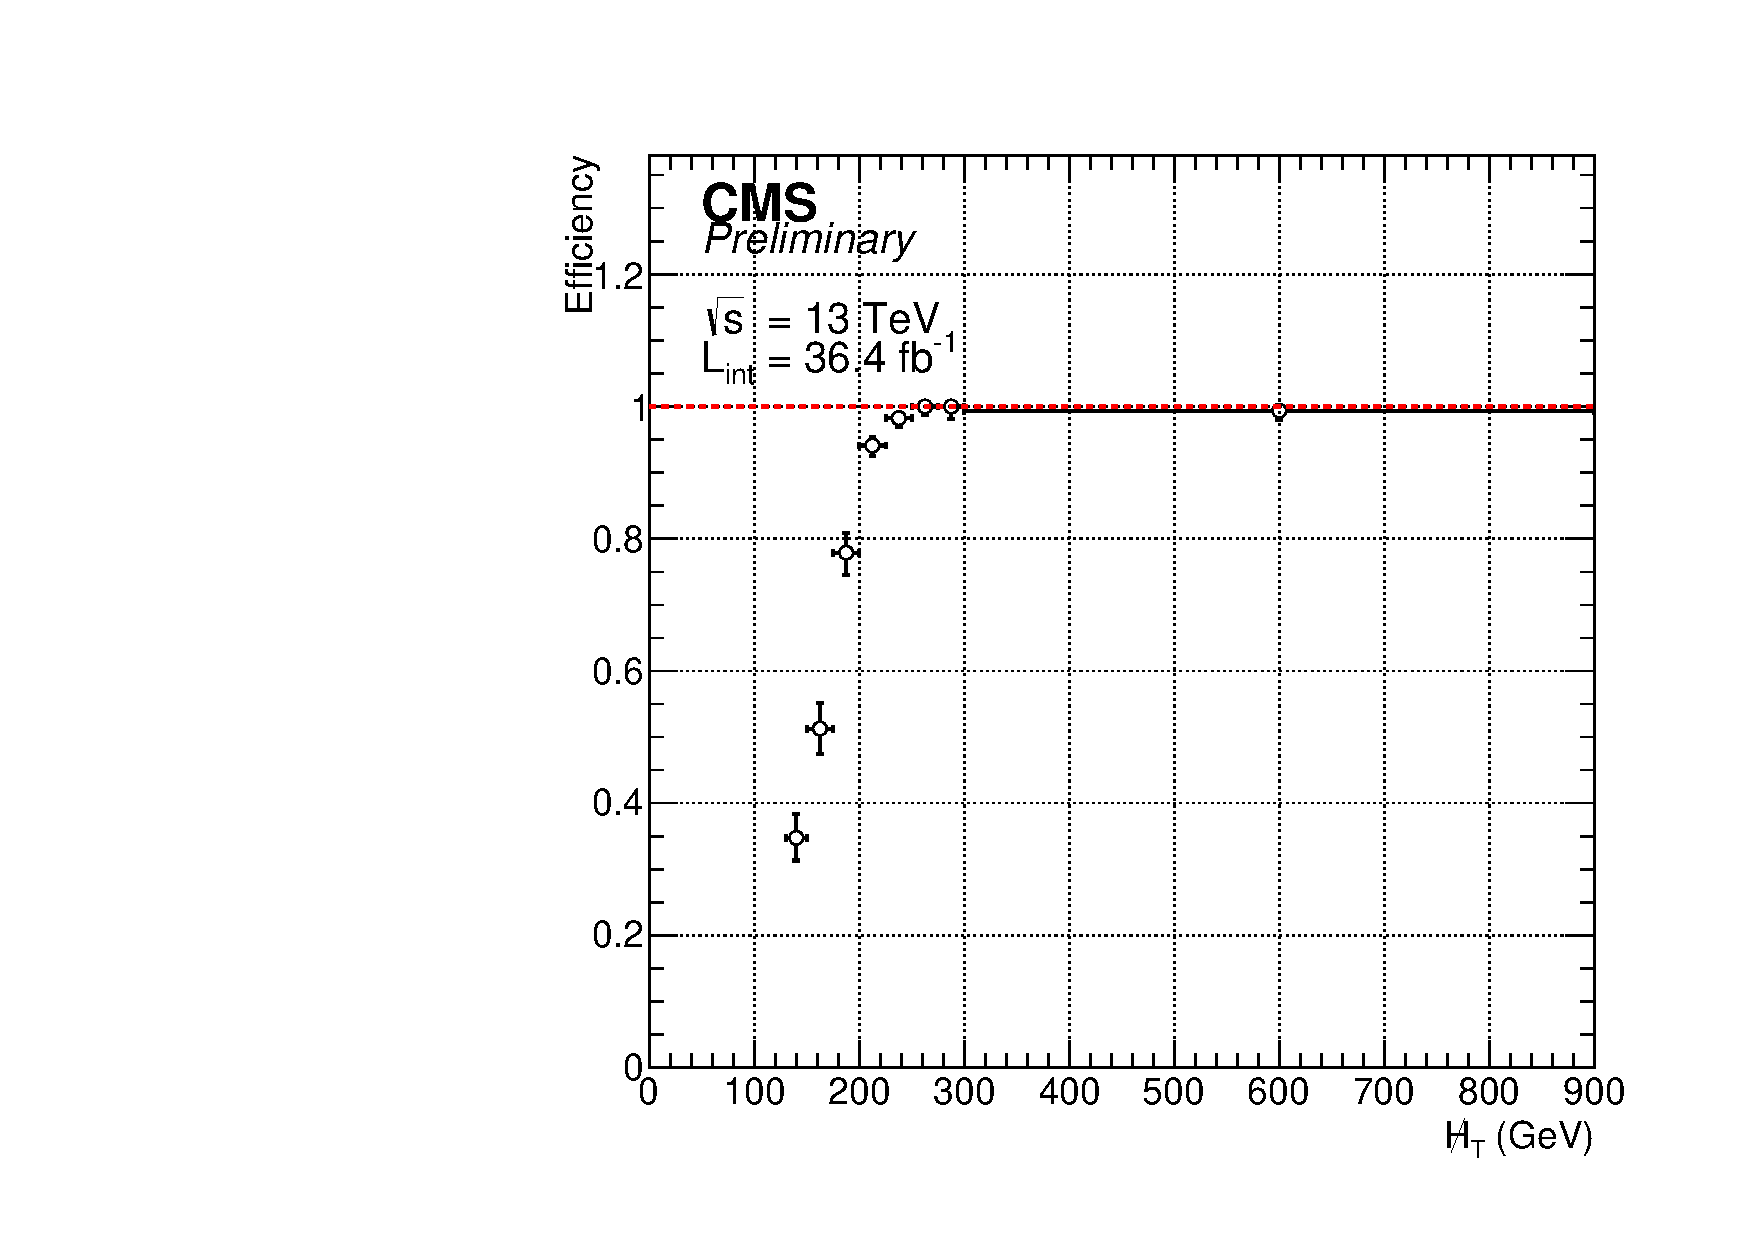
\includegraphics[width=0.26\textwidth]{figs/analysis/Trigger_Ele_HLT_AlphaTHT800MonoAll_MoM_all_200to400_mht}}
~
\subfloat[$200 < \scalht < 
400$~GeV]{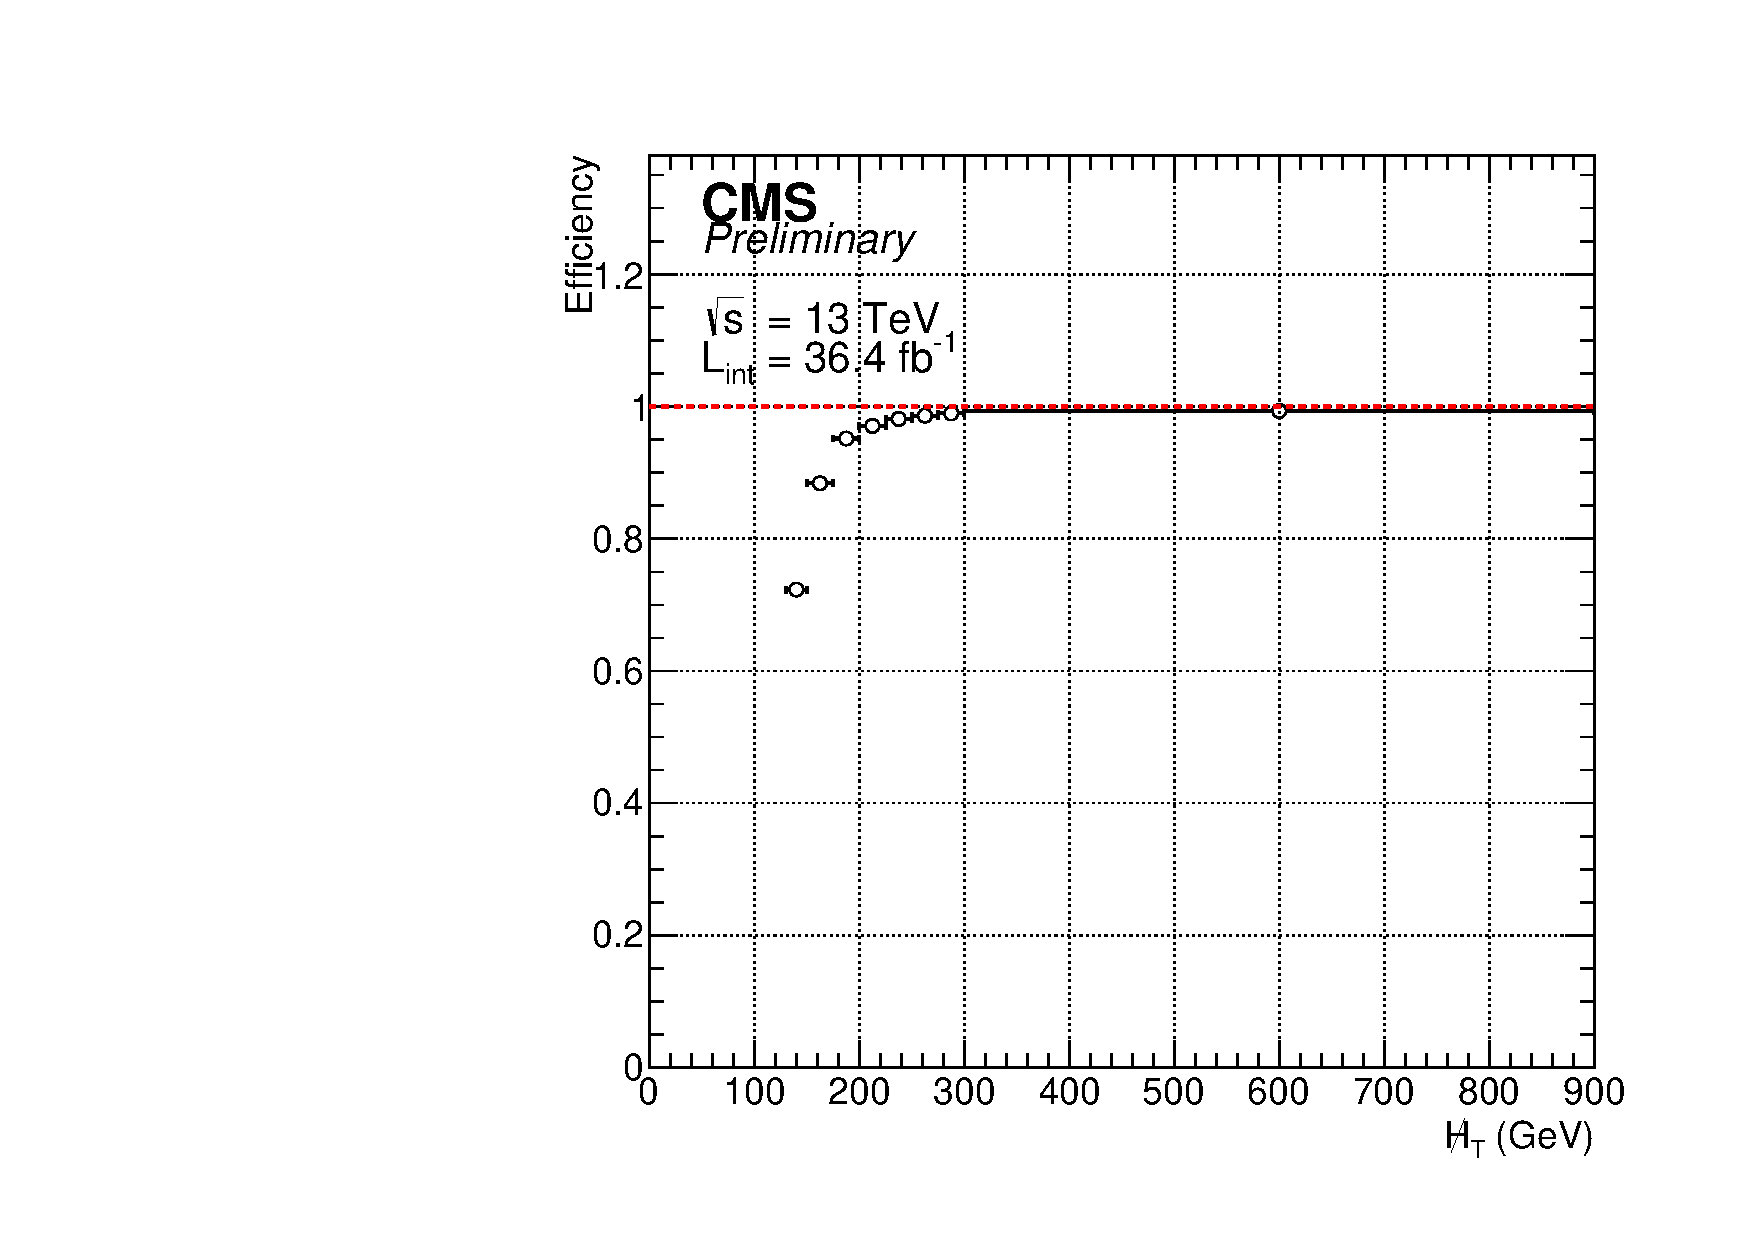
\includegraphics[width=0.26\textwidth]{figs/analysis/Trigger_Muon_HLT_AlphaTHT800MonoAll_MoM_all_200to400_mht}}
\\
\subfloat[$400 < \scalht < 
600$~GeV]{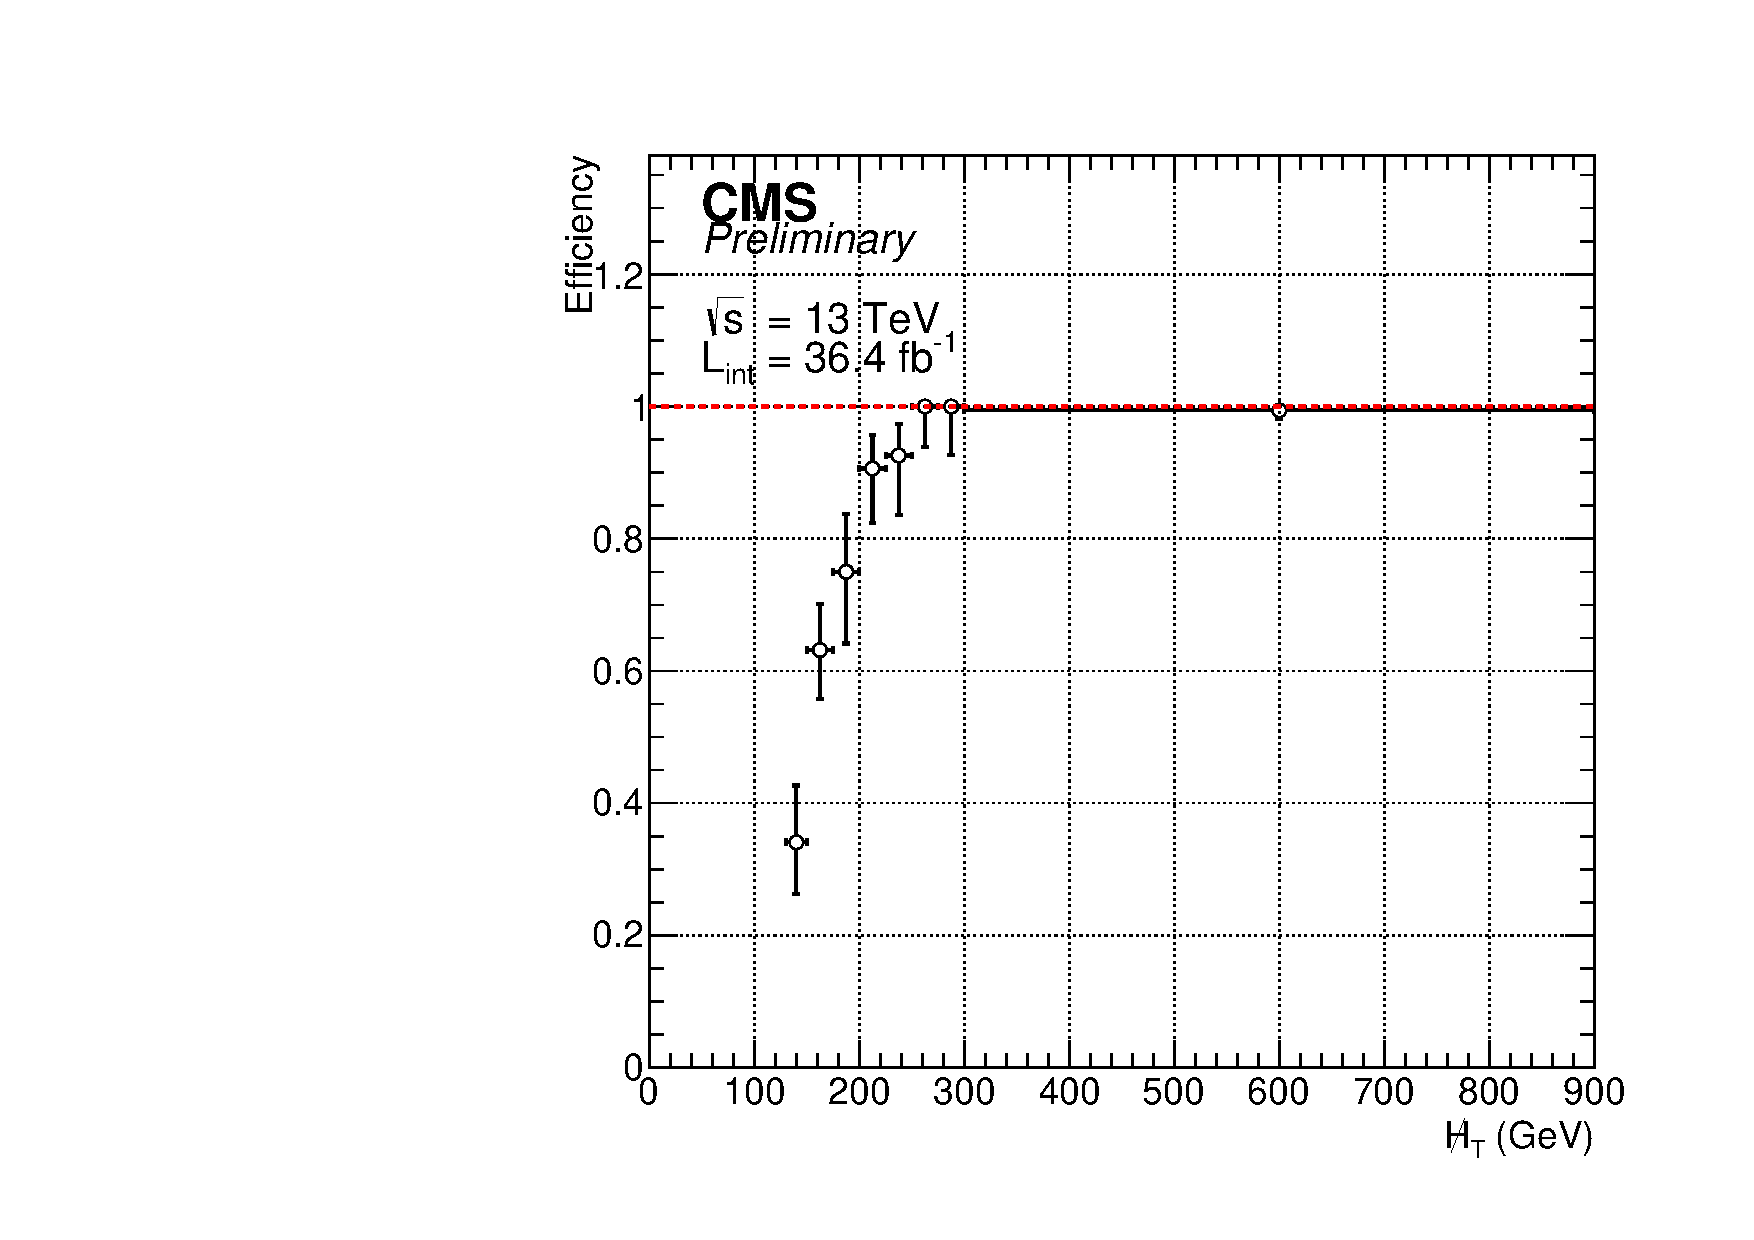
\includegraphics[width=0.26\textwidth]{figs/analysis/Trigger_Ele_HLT_AlphaTHT800MonoAll_MoM_all_400to600_mht}}
~
\subfloat[$400 < \scalht < 
600$~GeV]{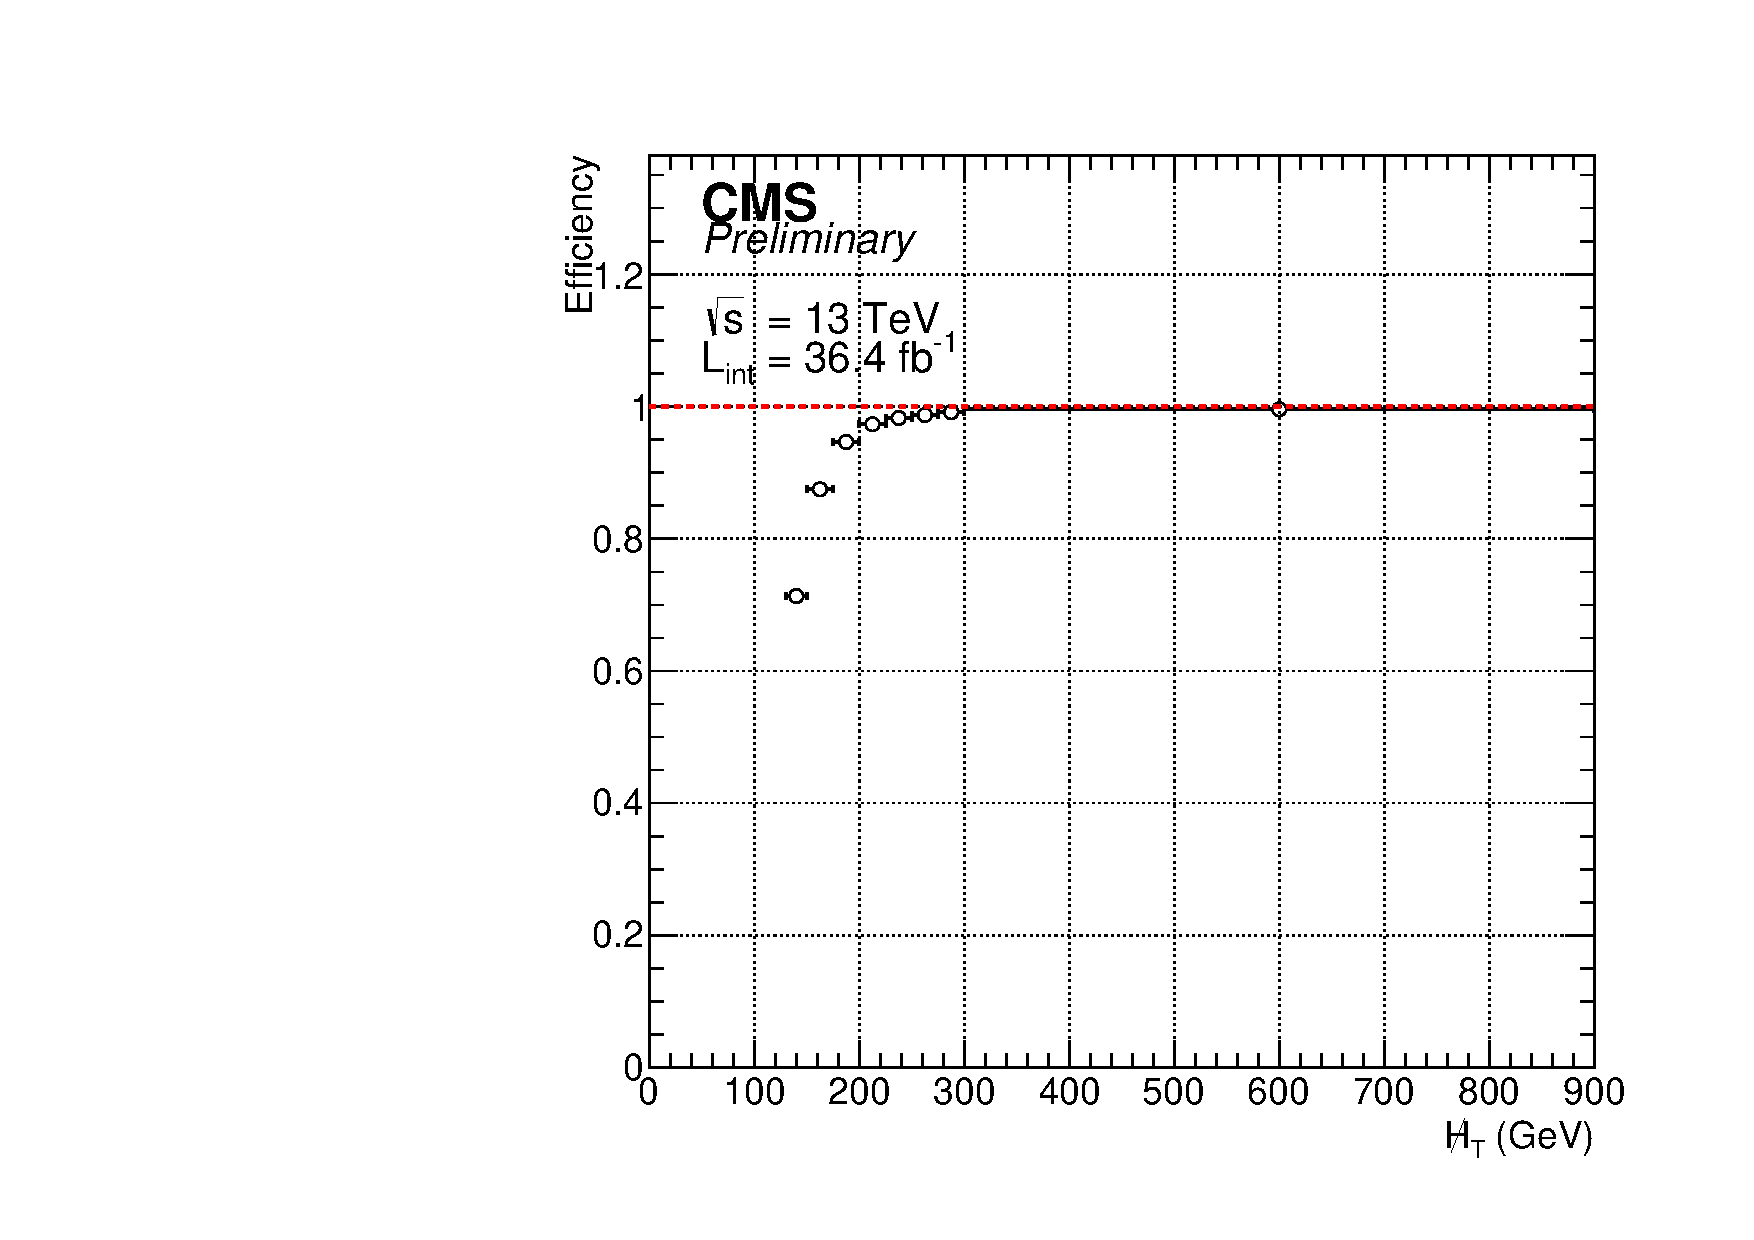
\includegraphics[width=0.26\textwidth]{figs/analysis/Trigger_Muon_HLT_AlphaTHT800MonoAll_MoM_all_400to600_mht}}
\\
\subfloat[$600 < \scalht < 
900$~GeV]{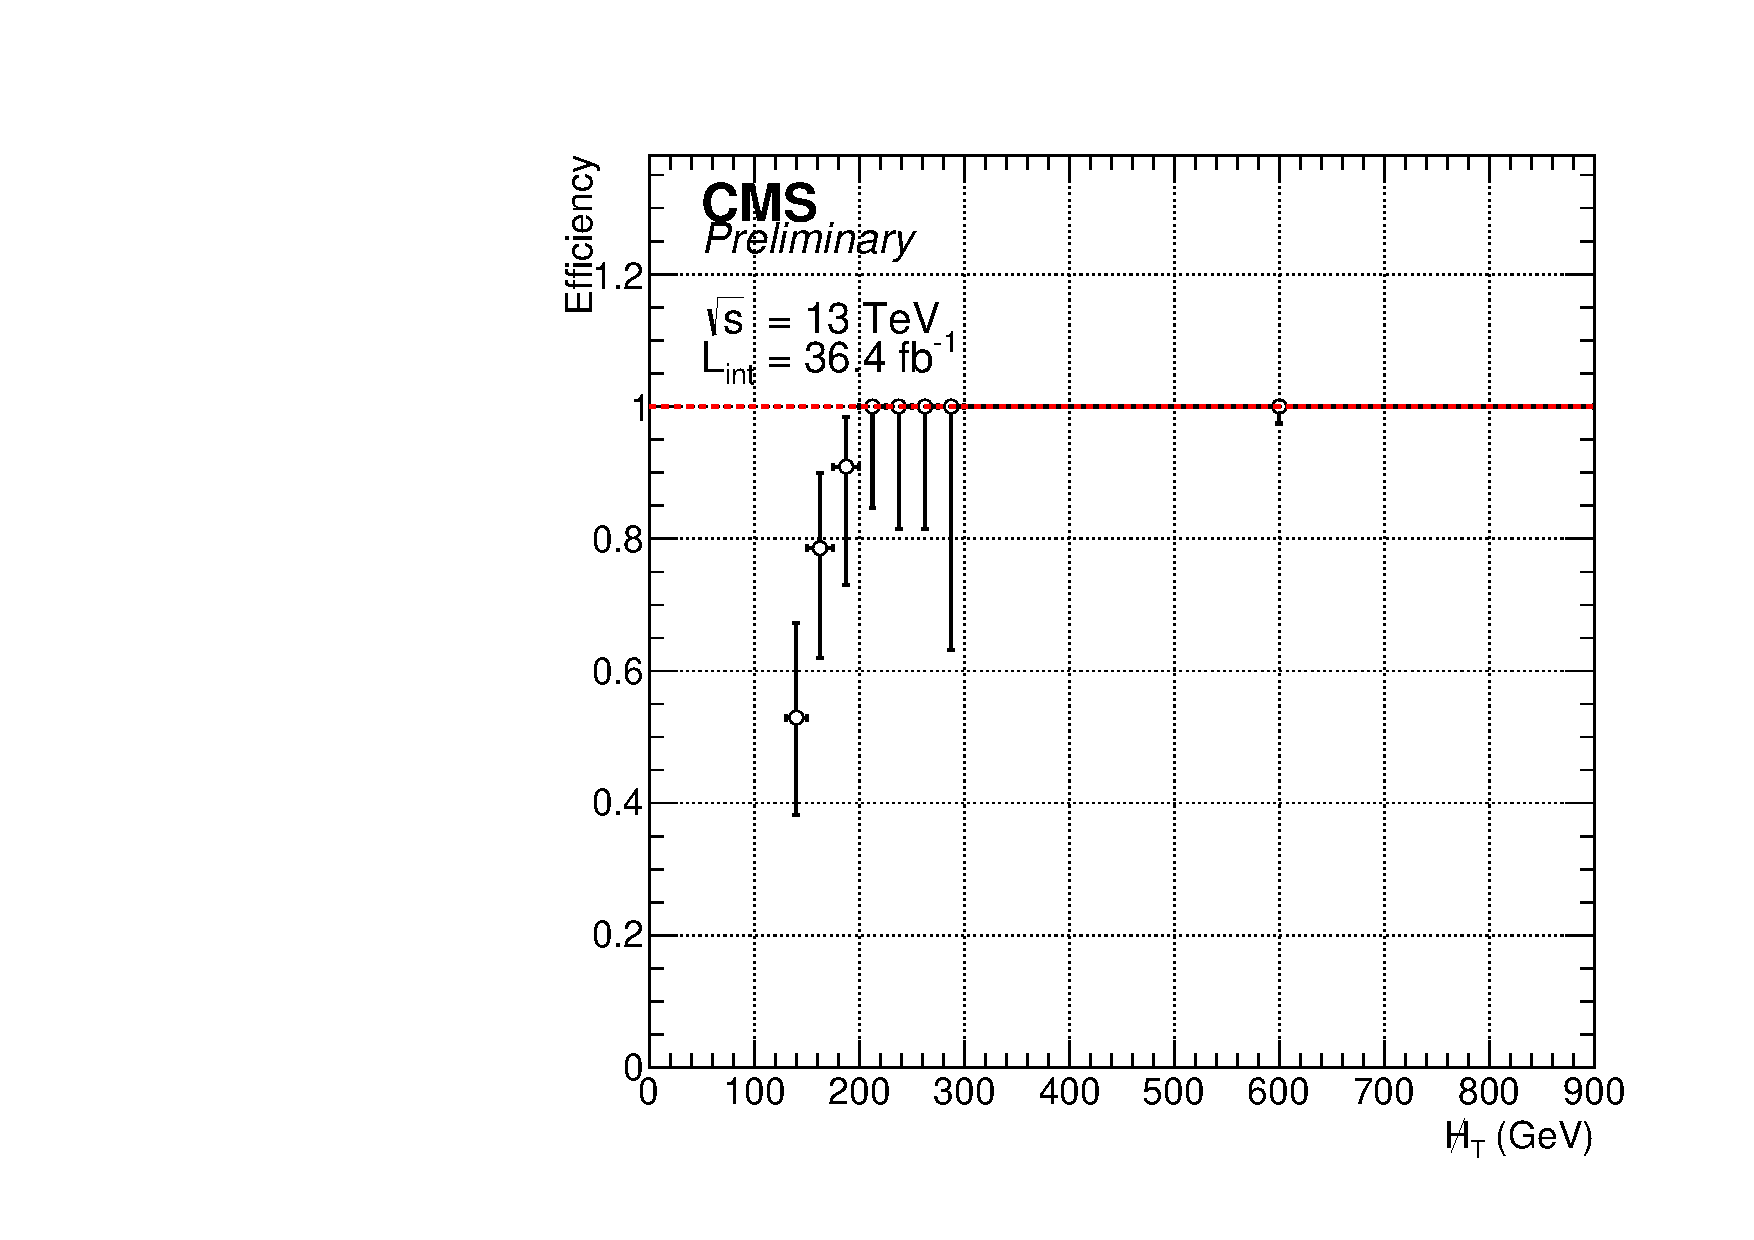
\includegraphics[width=0.26\textwidth]{figs/analysis/Trigger_Ele_HLT_AlphaTHT800MonoAll_MoM_all_600to900_mht}}
~
\subfloat[$600 < \scalht < 
900$~GeV]{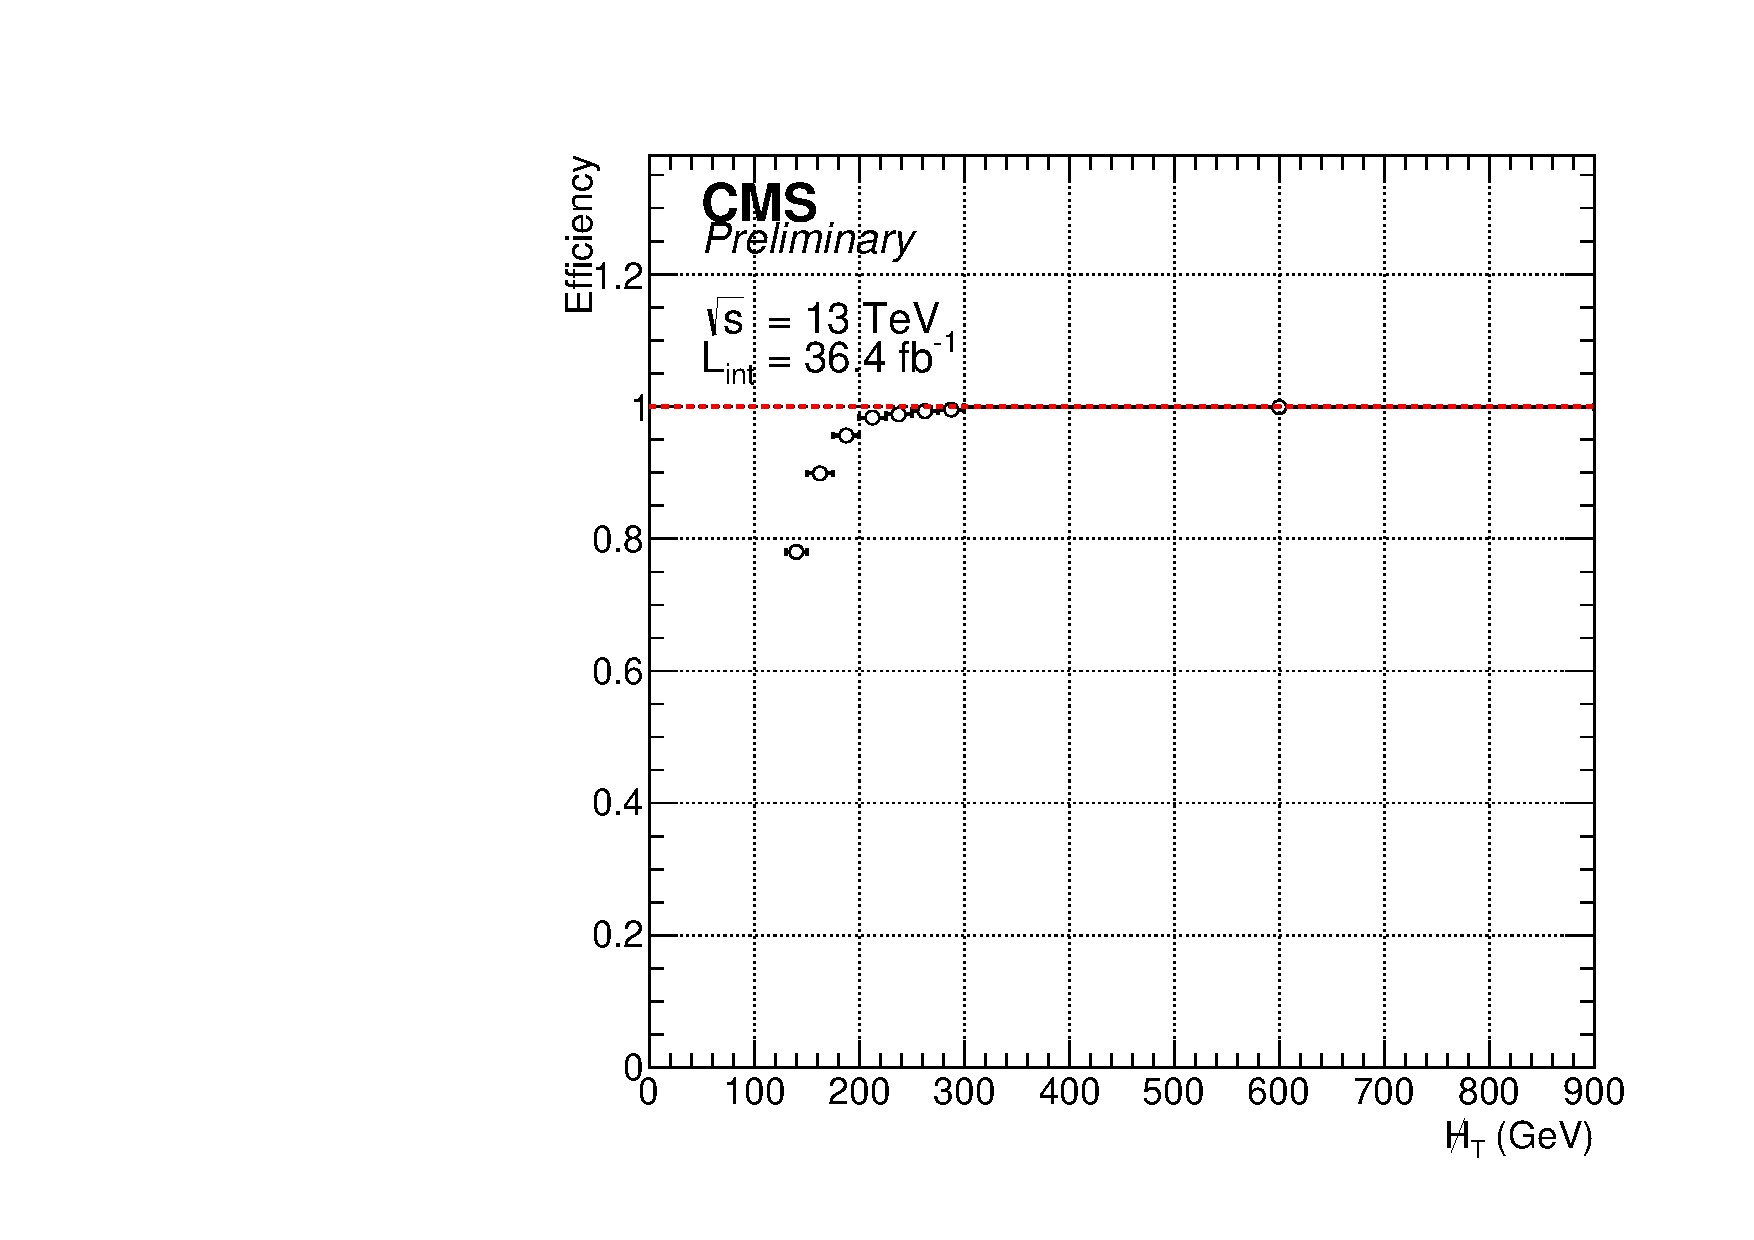
\includegraphics[width=0.26\textwidth]{figs/analysis/Trigger_Muon_HLT_AlphaTHT800MonoAll_MoM_all_600to900_mht}}
\\
\subfloat[$\scalht > 900$~GeV]      
{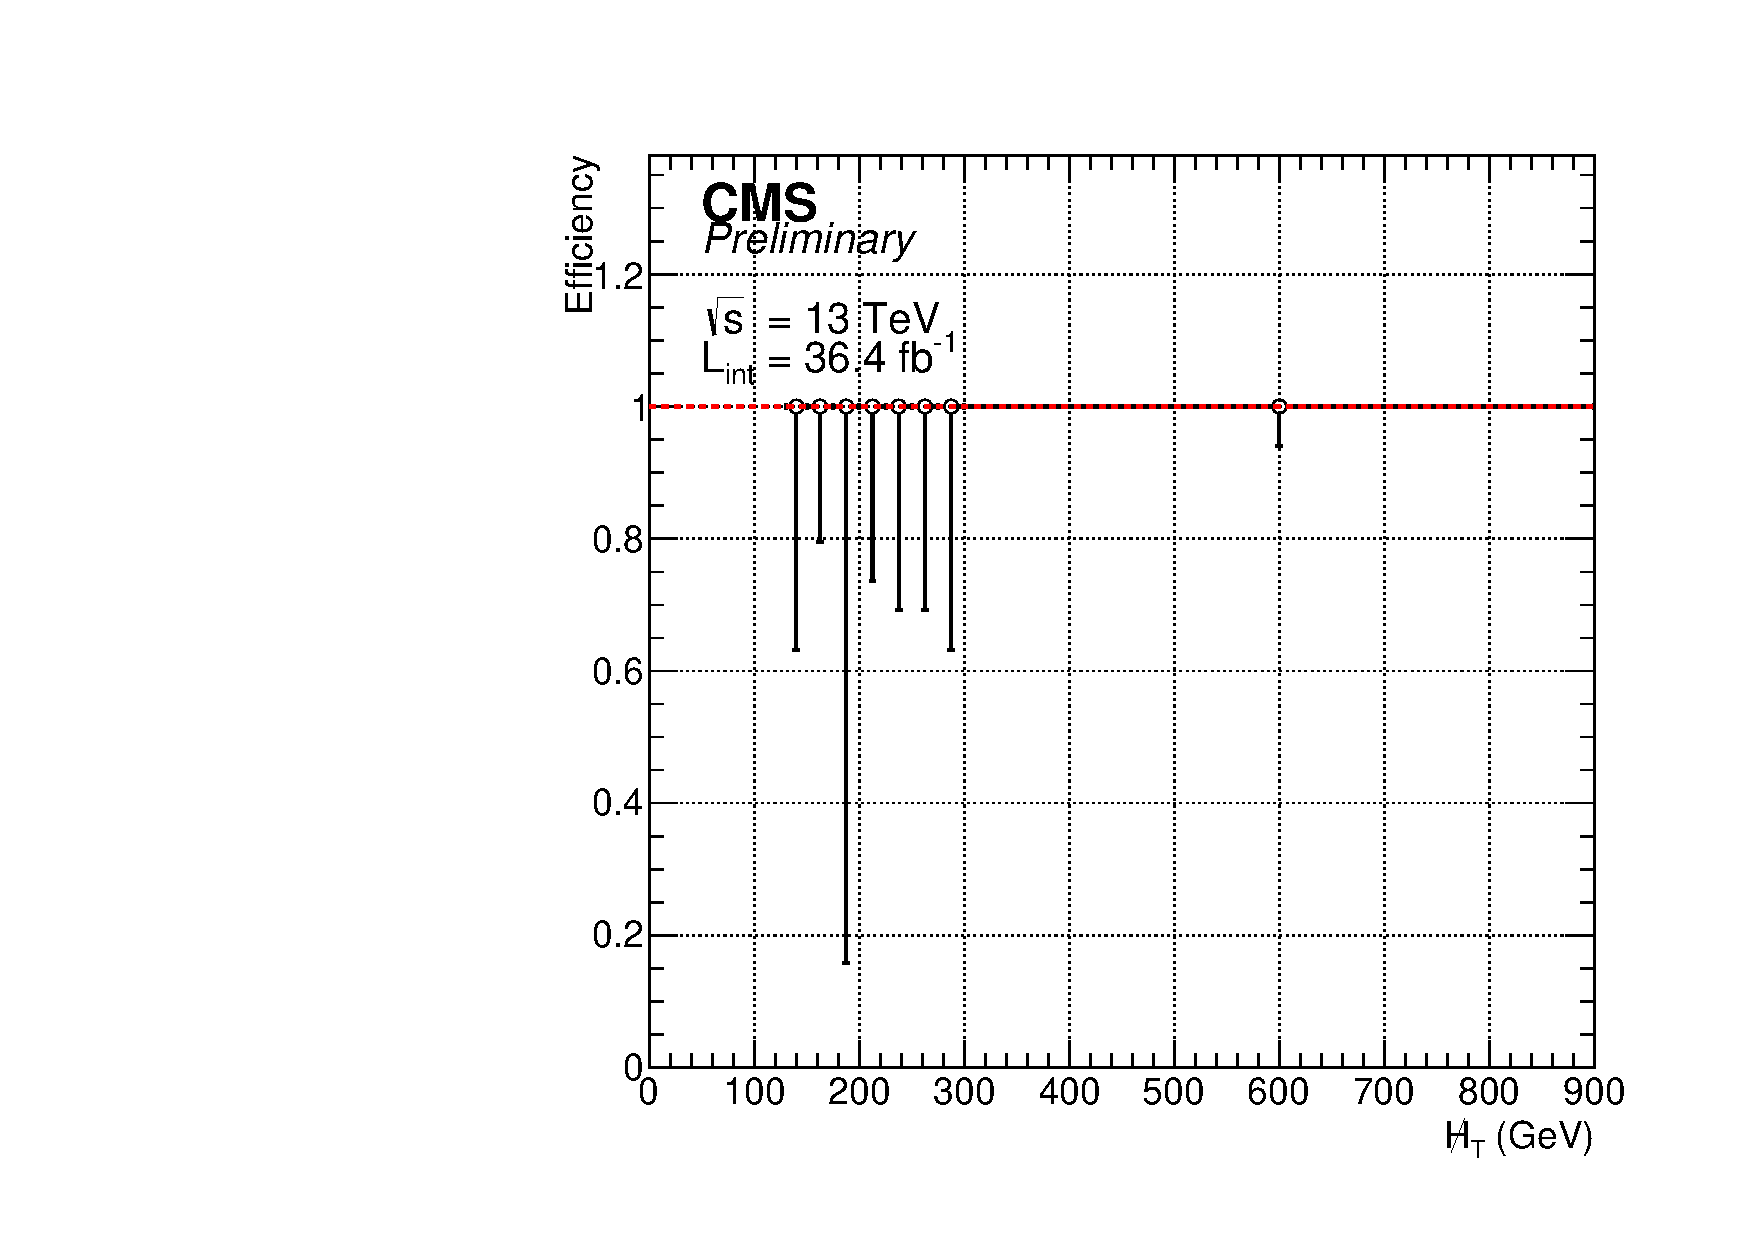
\includegraphics[width=0.26\textwidth]{figs/analysis/Trigger_Ele_HLT_AlphaTHT800MonoAll_MoM_all_900to999999_mht}}
~
\subfloat[$\scalht > 900$~GeV]      
{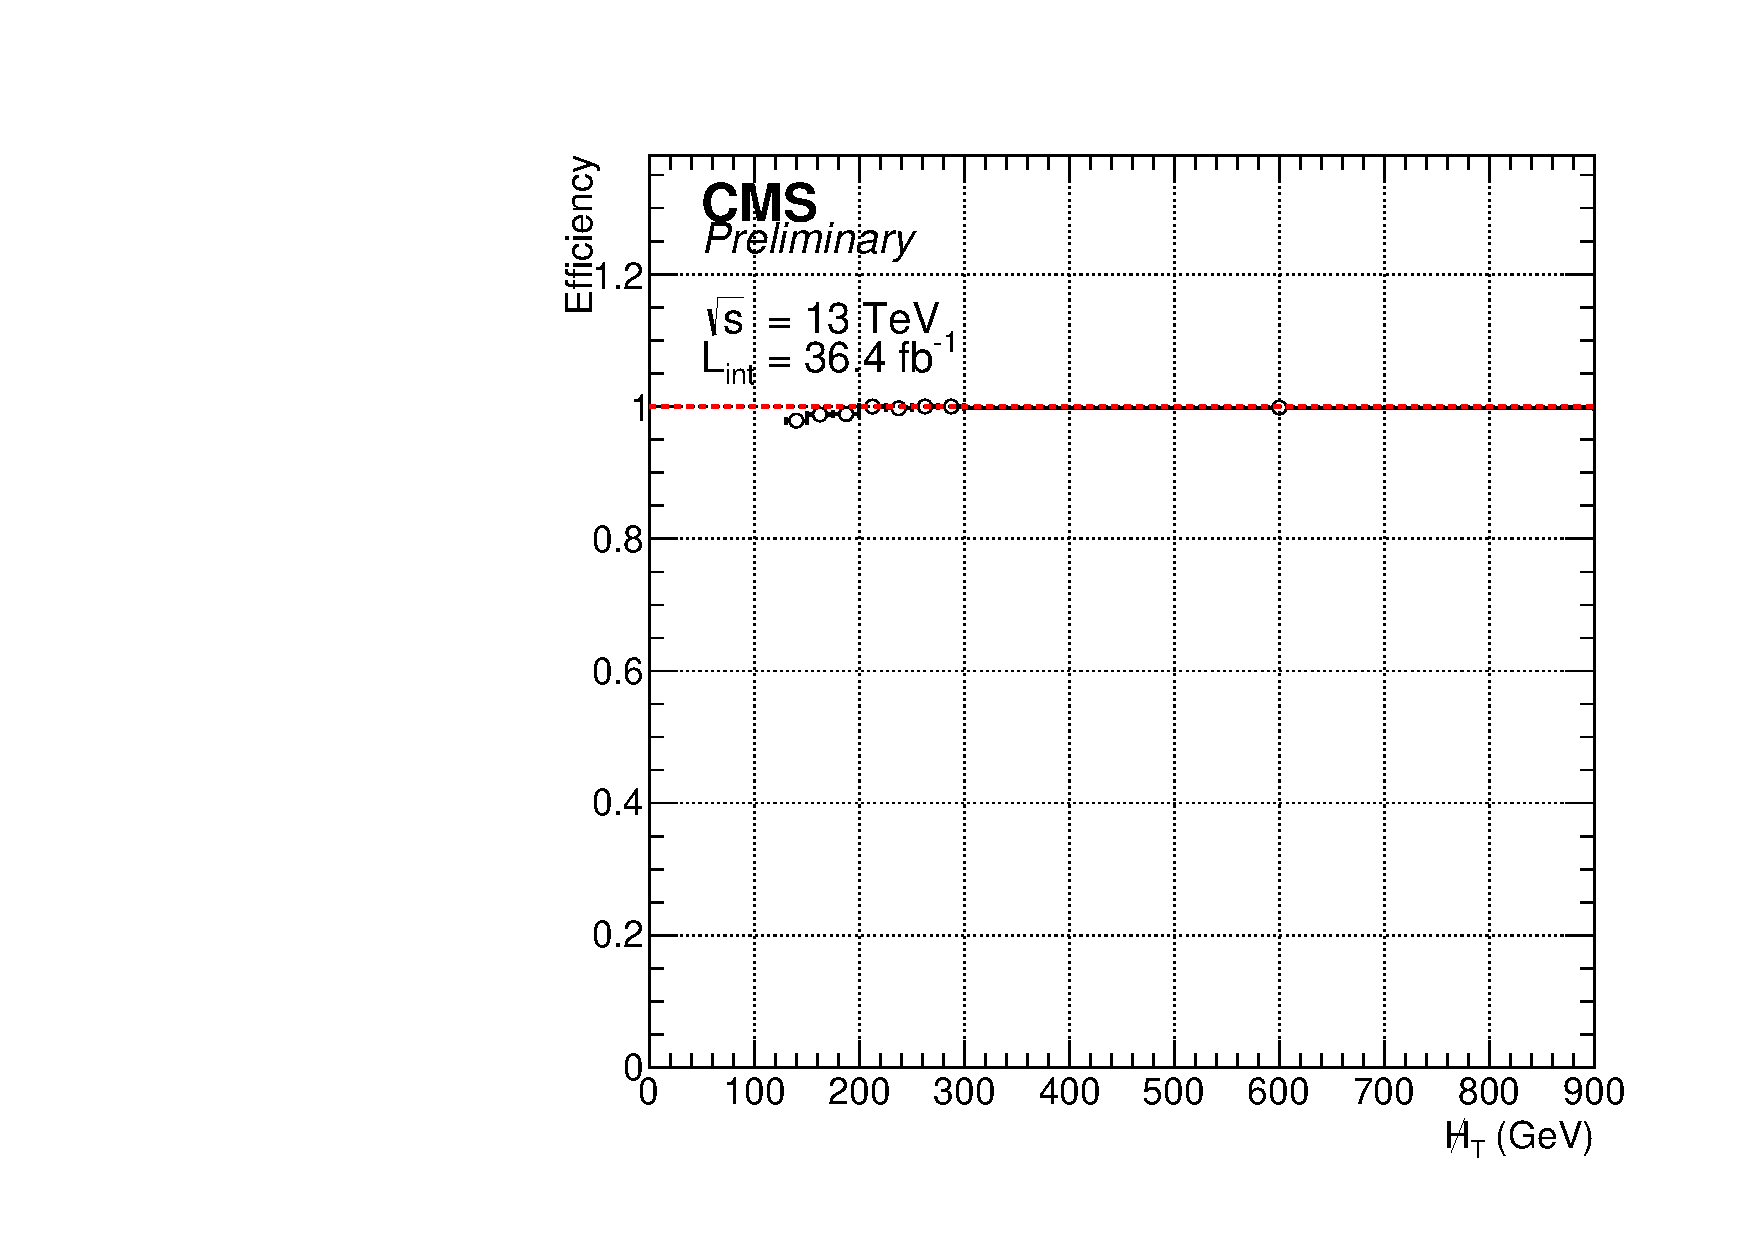
\includegraphics[width=0.26\textwidth]{figs/analysis/Trigger_Muon_HLT_AlphaTHT800MonoAll_MoM_all_900to999999_mht}}
\\
\caption{Efficiency of the HL trigger in the signal region as a function of 
offline \mht and \scalht, measured in a data sample collected by a single 
electron (left) and single muon (right) trigger.}
\end{figure}

This section has focussed on the signal region triggers. The efficiency of the 
muon trigger is also measured in data and used to correct the trigger 
efficiency in the simulation. This will be discussed further in 
Sec.~\ref{sec:analysis-mccorrections}.

%Efficiencies. Define with equation, in terms of reference trigger. Estimate 
%efficiency parameter. 
%Importance is because affects background estimations. 
%Need to correct simulation (see later) (not emulated in MC); also to to check 
%triggers are performing well obv.
%8 plots.
%Differences between muon and electron clear in turnon. Previously had 130 
%threshold but because of this raised to 200. Otherwise too much uncertainty 
%about true efficiency which could lead to bias in background estimation
%Say why efficiency is not necessarily 100 per cent - L1 inefficiency, 
%prefilter inefficiency (coarse information), not exactly same objects as 
%offline (e.g. 30 GeV jets), alphat is not exactly mht.
%Measure in data to avoid MC mismodelling. 
%Leptonic triggers are best because 
%are unbiased/no selection of MET (when lepton ignored - just like W 
%background (e.g. HT trigger eff appears better than it really is if you count 
%the muon as a jet - but we are interested in the eff for events with no 
%muons). 
%Could use prescaled HT triggers (and would include Zinv not just W) but 
%prescales too large so too large uncertainties. 
%Anyway efficiencies are close to 100\% so any bias is covered with a 
%conservative systematic unc, and met trigger is as good or better in most of 
%phase space and there is no bias for that one.
%Bias from closs-cleaning inconsistencies in the L1-HLT-offline chain. Table 
%like mark yes no.
%Can use electron for consistent chain but topology doesn't really represent 
%that of SR.
%Remember METNoMu does have cross-cleaning so not affected.

%Eff for signal models is checked in simulation and is close tp 100\%.
%Same triggers used in hadronic control regions (mhtmet caveat)

%Two ways of doing muon cross cleaning in HLT (Mark): just reconstruct muon and 
%apply deltaR cleaning (as offline) or remove jet if muon energy fraction is 
%greater than 0.6


\section{Data sets and simulation samples}
\label{sec:analysis-samples}
%0.5 pages.
%Maybe put here the "datasets" section of data and MC samples (see Matt).
This section describes the data sets in which the search for SUSY and DM takes 
place, as well as the simulated data sets that aid in the estimation of the 
background and signal processes.

% both data and MC stored as ROOT trees with an entry per collision event, all 
%important reco information stored per event

\subsection{Data sets}
\label{sec:analysis-samples-data}

Between 22$^\mathrm{nd}$ April 2016 and 27$^\mathrm{th}$ October 2016, the 
LHC delivered a total integrated luminosity of 40.8~\ifb of proton-proton 
collisions at a centre of mass energy of \com with a proton bunch spacing of 
25~ns. Of this, 37.8~\ifb (93\%) was recorded by the CMS detector, and 
35.9~\ifb (88\%) was certified as containing data of good quality, meaning 
there were no associated detector or reconstruction issues. The amount of data 
delivered, recorded and certified over the year is shown in 
Fig.~\ref{fig:lumi}.
It is the certified 35.9~\ifb of data that form the basis of the search. The 
data sets that are analysed correspond to those collected by the triggers 
described in Sec.~\ref{sec:analysis-trigger}.
%The uncertainty on the certified integrated luminosity is 2.x\%
%\textbf{TODO: lumi uncertainty and reference (or just leave for corrections 
%section).}
%Each family of triggers collects a subset of these data, and these are stored 
%as separate files which can then be processed further and analysed.
% aod - miniaod - trees

\begin{figure}[!htb]
\label{fig:lumi}
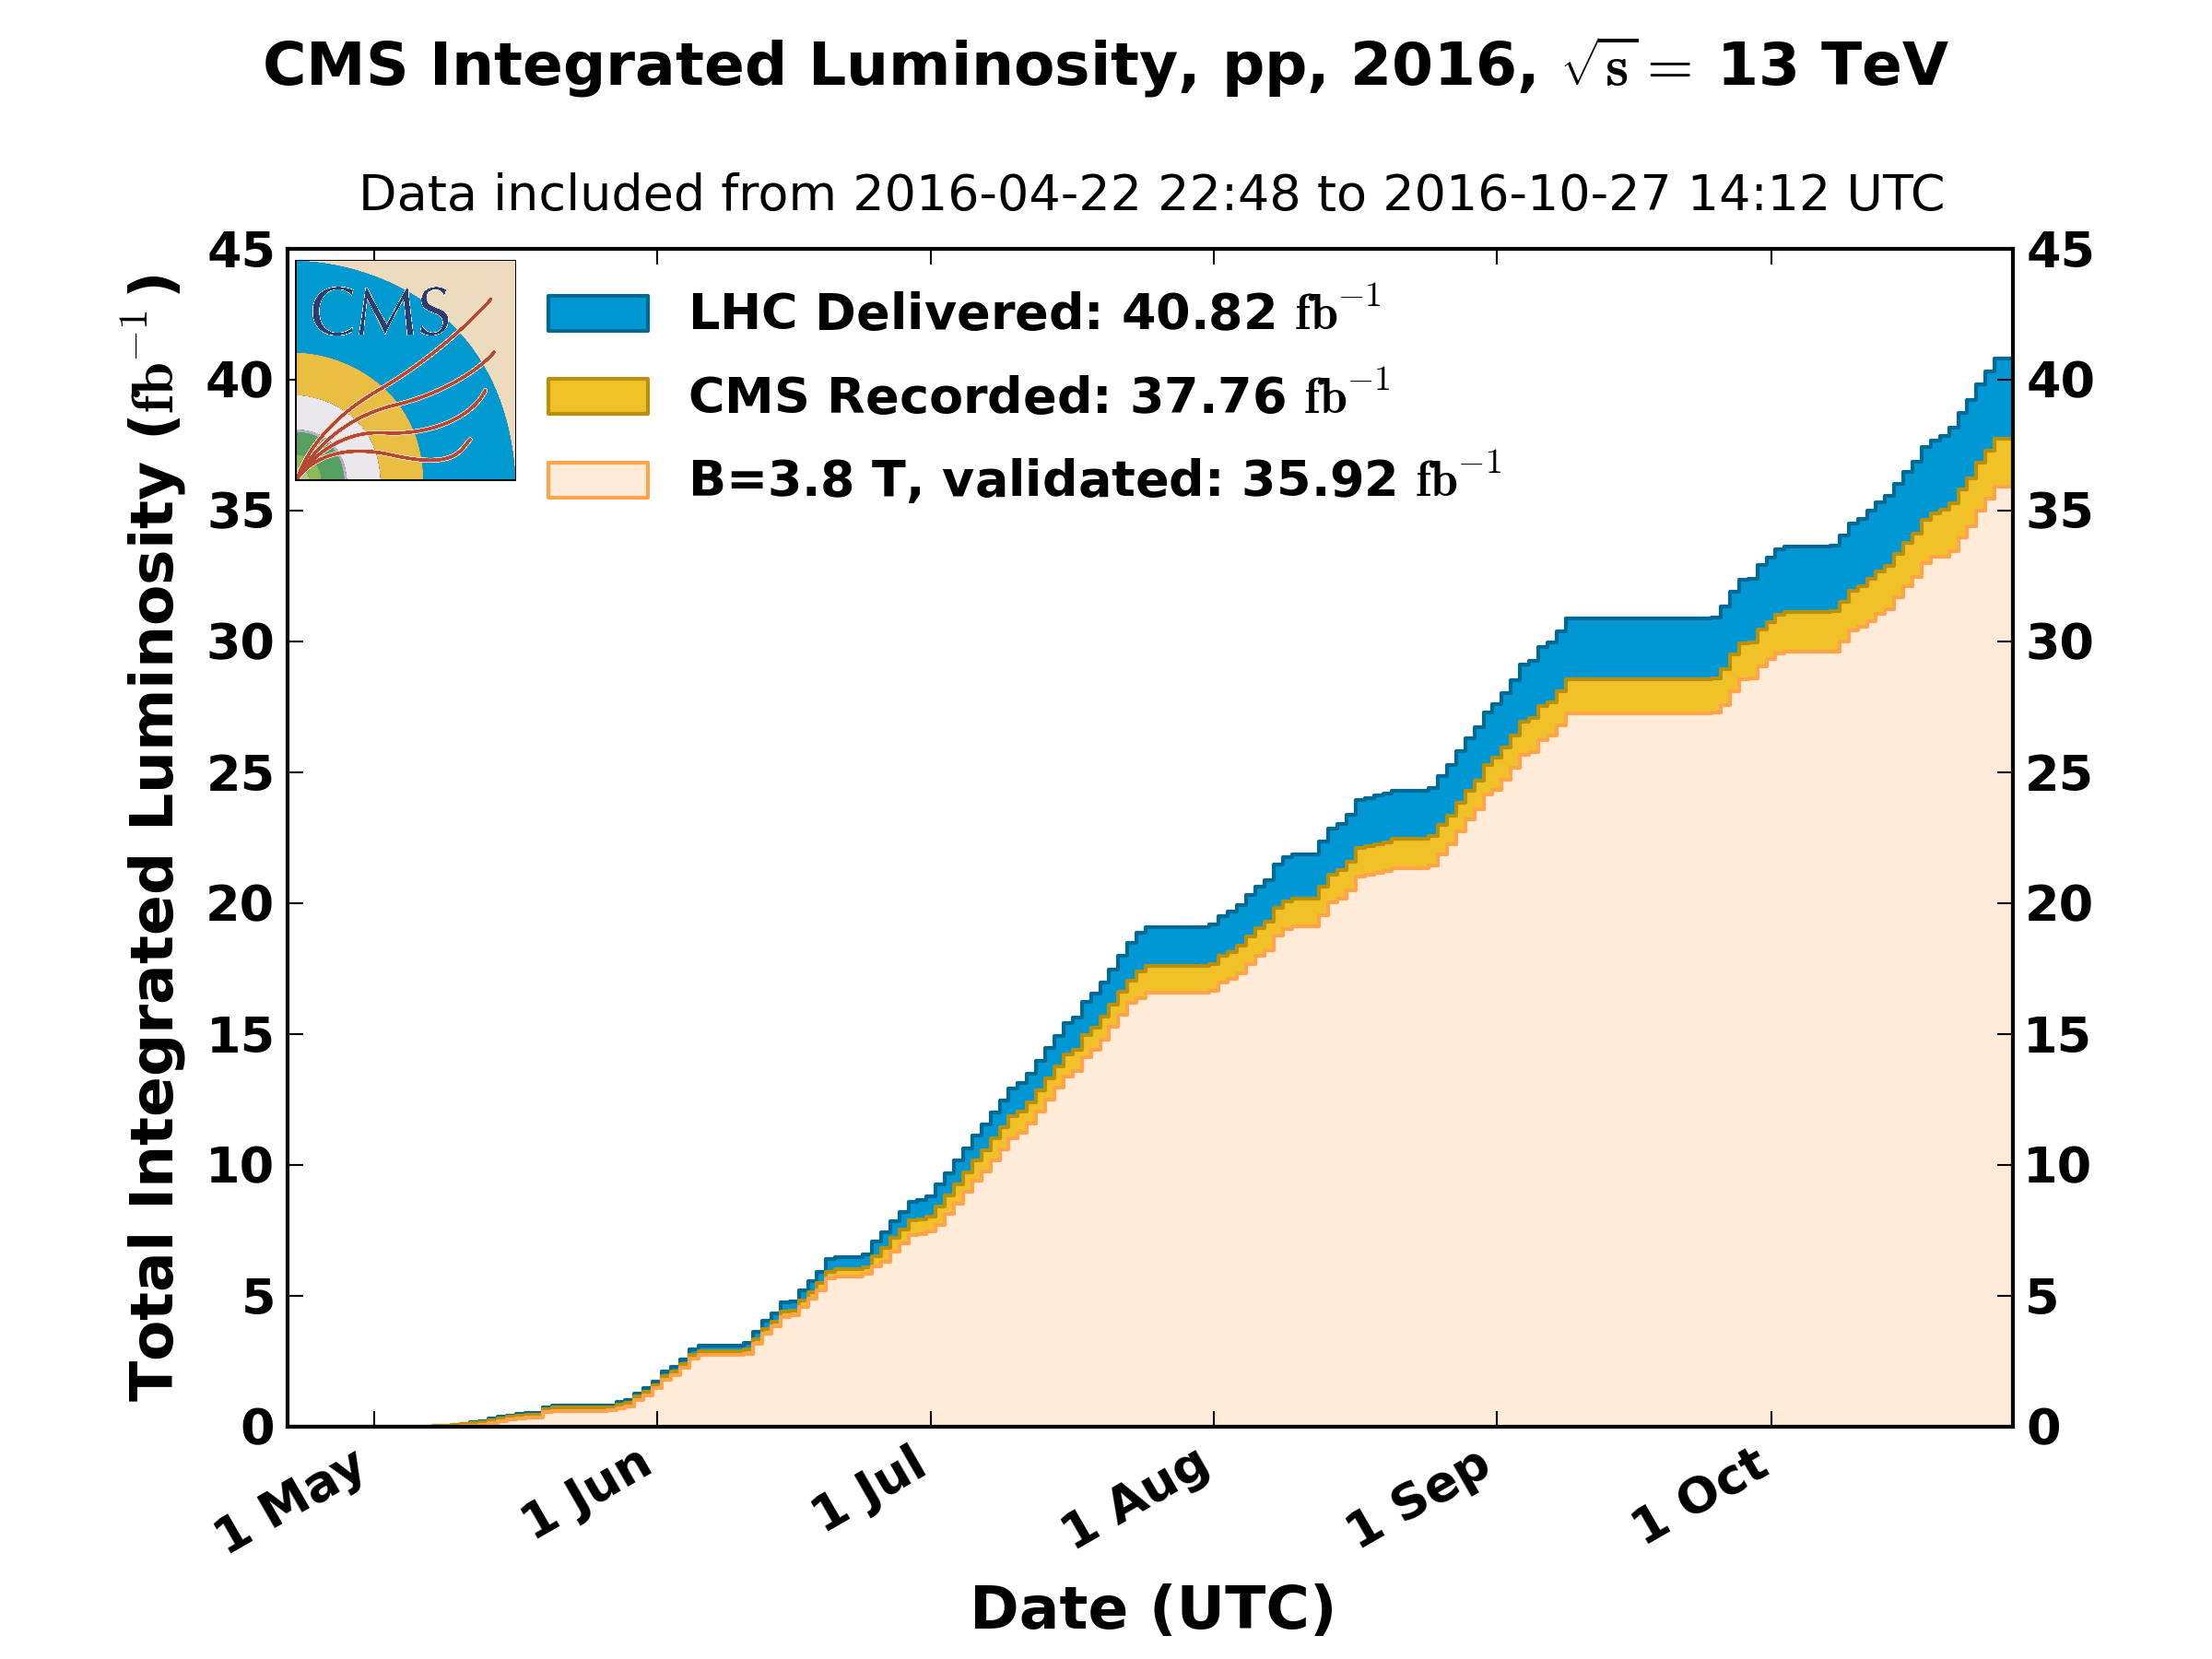
\includegraphics[width=0.7\textwidth]{figs/analysis/cmslumi}
\caption{Cumulative integrated luminosity of pp collisions at \com delivered by 
the LHC, recorded by CMS, and certified as good for physics analysis per day 
during the year 2016~\cite{cmslumi16}.}
\end{figure}

%runs (2016B etc), certification, primary datasets. 25ns.

\subsection{Simulation samples}
\label{sec:analysis-samples-mc}

The methods of Monte Carlo event generation, hadronisation and detector 
simulation were described in Sec.~\ref{sec:detector-simulation}.
The Monte Carlo generation of the main background processes (QCD, \zj, \wj, 
\ttbar) is produced via the \textsc{MadGraph5}~\cite{madgraph5} generator 
framework at leading order (LO) precision. 
% also DY (same as Zjets)
As the number of events falls exponentially with the energy scale of the event, 
and it is the most energetic events that typically pass the signal region 
requirements, these samples are generated in various bins of \hthat, the total 
hadronic energy of the partons produced in the hard scattering. 
%The \hthat sub-samples all contain approximately the same number of events
%several parton ht bins to improve stats (exponential to flat), reweight)
This improves the statistical precision of the simulation in the phase space 
region of interest.
Single top quark production is generated at next-to-leading order (NLO) using 
both \textsc{MadGraph5} and \textsc{powheg}~\cite{powheg} for the different 
production channels. The diboson background is generated with 
\textsc{pythia8}~\cite{pythia8}.
While events are generated at LO or NLO, the cross sections of most of the main 
background processes are computed at next-to-next-to-leading order (NNLO) 
precision~\cite{adam-lots}.
%\textbf{TODO no need to mention pythia hadronisation and geant here?}

The SUSY and DM signal samples are generated with \textsc{MadGraph5}. For each 
model, various masses and lifetimes of the relevant particles are generated. 
This allows for the sensitivity of the search to be explored as a function of 
these variables.
The \verb|T1qqqq| model with a promptly-decaying gluino is simulated via a 
\textit{fast simulation} framework which employs a simplified detector geometry 
and smearing of the particles' four-vectors, enabling it to perform $\sim$100 
times faster than a full simulation with \textsc{geant} but with comparable 
accuracy~\cite{fastsim}.
%prompt fastsim (see my description in 9M?), ll fullsim

%SUSY xs NLO+NLL.
\textbf{TODO: RHADRONS (see paper), baryon and meson states, gluino ball - 
maybe this will described in simplified models section.}

%table of samples? not necessary (but familiarise with it and xs)

Based on simulation, the estimated number of events of a given process with 
cross-section $\sigma$ is given by:
\begin{equation}
\hat{n}_\mathrm{sim} = \sigma L \frac{N_{\mathrm{pass}}}{N_{\mathrm{gen}}}
\end{equation}
where $L$ is the integrated luminosity, $N_{\mathrm{gen}}$ is the number of 
events generated, and $N_{\mathrm{pass}}$ is the number of events that pass the 
analysis selections.


\section{Corrections to simulation}
\label{sec:analysis-mccorrections}
%3-5 pages
This section describes various ways in which the potential mismodelling of the 
simulation is corrected for. This usually involves observing a distribution or 
measuring an efficiency both in data and simulation and applying the 
data-to-simulation ratio as a weighting factor to each simulated event. These 
corrections are applied to the simulation of both background and signal 
processes, as relevant.
There are uncertainties associated with each set of correction factors, the 
treatment of which is detailed in Sec.~\ref{sec:analysis-systematics}.
%Simulation modelling is not perfect. Need to correct it using scale factors by 
%comparing data and MC. These corrections introduce systematic uncertainties in 
%the background estimation, that will be described later in Sec X.

Mention typical size of weights in each subsection.

\subsection{Pileup}

The average number of pileup interactions per bunch crossing during the 2016 
run was $\sim$20. The pileup distribution depends on the instantaneous 
luminosity, which varies over time, and so is not reproduced very accurately by 
the simulation.

Reweighting factors to correct the pileup distribution in the simulation are 
derived as a function of the number of pileup interactions. The pileup in a 
given event in data is calculated from the average instantaneous luminosity 
measured in the corresponding luminosity section, together with the inelastic 
proton-proton cross section (63~mb~\cite{inelasticxs-atlas13tev}). The 
correction factors are given by the ratio of the pileup distributions in data 
and simulation. These range between $\sim$0.8-1.2 in the bulk of the 
distribution.
% distributions are normalised to normalisation of MC conserved

\textbf{TODO: maybe put pileup reweighting plot (AN).}

\subsection{b-tagging}
\label{sec:analysis-corrections-btagging}
% https://twiki.cern.ch/twiki/bin/viewauth/CMS/BTagSFMethods

The efficiency for identifying jets as originating from a bottom quark tends to 
be overestimated in the simulation. Similarly, the probability of incorrectly 
b-tagging a jet that actually originated from a light flavour (u, d, s) quark 
or gluon is underestimated. Correction factors for the b-tagging efficiency and 
fake rate are therefore derived, in bins of jet \pt and $\eta$, and applied to 
the simulation.

The b-tagging probability 
%(b-tagging efficiency (or mistagging probability) 
for a jet originating from a quark (or gluon) of flavour $q$ with transverse 
momentum \pt and pseudorapidity $\eta$ is estimated as:
\begin{equation}
\label{eqn:btag-eff}
\varepsilon(\pt, \eta, q) = \frac{N_{\text{b-tagged}}(\pt, \eta, 
q)}{N_{\text{total}}(\pt, \eta, q)} \, ,
\end{equation}
where $N_{\text{total}}(\pt, \eta, q)$ is the total number of jets of true 
flavour $q$ in bin (\pt, $\eta$) and $N_{\text{b-tagged}}(\pt, \eta, q)$ is 
the number of such jets that are b-tagged.
The flavour $q$ is labelled as one of three types --- b, c, or light (u, d, 
s, or gluon).

% In simulation, generator information gives jet flavour
In simulated events, the true flavour of a jet is determined according to 
whether there are any bottom or charmed hadrons contained within the jet's cone.
%using generator-level information.
In data, the b-tagging efficiency is measured in a sample of \ttbar events or 
jets containing a muon, and the mistagging probability is measured using jets 
with a negative impact parameter or negative decay 
length~\cite{btagging-cms-run2}.
% 2 methods:
% use jets with muons inside (ptrel method)
% select ttbar events, predict background, do complex likelihood fit
The ratio of the b-tagging probability in data and simulation provides a 
correction factor $f(\pt, \eta, q)$ that is used to weight the events from 
simulation.
The correction factors are in the range $\sim$0.95–1 and $\sim$1–1.2 for bottom 
quarks and light partons, respectively.
%for a jet-pT range of 40–600GeV.

While the correction factors derived in Ref.~\cite{btagging-cms-run2} are for 
an inclusive set of jets, the b-tagging probabilities are also measured in 
the signal and control regions of the search. Given these probabilities and the 
correction factors, for each simulated event the probability of observing the 
corresponding combination of tagged and non-tagged jets in data and simulation 
is computed as:
\begin{equation}
P_\text{sim} = \prod_{j~\text{b-tagged}} \varepsilon_{j} 
\prod_{j~\text{not 
b-tagged}} (1 - \varepsilon_{j})
\end{equation}
\begin{equation}
P_\text{data} = \prod_{j~\text{b-tagged}} f_{j} \varepsilon_{j} 
\prod_{j~\text{not 
b-tagged}} (1 - f_{j} \varepsilon_{j})
\end{equation}
where $\varepsilon_{j} \equiv \varepsilon(\pt(j), \eta(j), q(j))$ is 
the probability of jet $j$ being b-tagged, as measured according to 
Eq.~\ref{eqn:btag-eff}, and $f_{j} \equiv f(\pt(j), \eta(j), q(j))$ is 
the corresponding correction factor. 
The simulated event is then weighted by the ratio:
\begin{equation}
w = \frac{P_\text{data}}{P_\text{sim}} \, .
\end{equation}

Signal models that are simulated via a fast simulation procedure are weighted 
according to correction factors that are derived to match the b-tagging 
probability in full simulation, and are then weighted again using the above 
procedure to match the b-tagging probability in data.
%(only for T1qqqq prompt).

%a plot? prob not

% https://twiki.cern.ch/twiki/bin/view/CMS/BTagSFMethods
% see btagging CMSDAS Introduction.pdf
% scale factors: either jet-by-jet or event reweighting
% all methods have pros and cons

\subsection{Muon identification, isolation and triggering}
%% and reconstruction
%% muon tracking eff (SFs are in sequence but syst not in stats code)
The efficiencies of the muon trigger and the muon identification and isolation 
requirements 
described in Sec.~\ref{sec:analysis-physicsobjects} are corrected for in 
the simulated events that enter the muon control regions. These efficiencies 
are measured in data and simulation using the \textit{tag-and-probe 
method}~\cite{tagnprobe} as explained in the following.
% point is need TnP for data, for MC could use truth info but need to use 
%consistent method

% eg Z, J/psi, upsilon
The tag-and-probe method takes advantage of a known mass resonance to identify 
particles of a desired type and evaluate various efficiency measures such as 
the ability to reconstruct or trigger such particles. In this case the 
particles of interest are muons and they are identified via the Z boson 
resonance. 
First, a muon that satisfies stringent quality criteria is selected and 
labelled as the \textit{tag}. A second muon satisfying looser requirements, 
labelled the \textit{probe}, is then paired with the tag if it is oppositely 
charged and the invariant mass of the pair is within a $\sim$30~GeV window 
around the Z boson mass. These requirements on the tag and probe mean that they 
are almost certainly real muons. It is then checked whether the probe satisfies 
the selection whose efficiency is of interest. An estimate of the efficiency is 
given by the fraction of probes that pass the selection. Note that a tag 
satisfies the probe requirements by definition, and so a dimuon event in which 
both muons are tagged contains two tag and probe pairs. A tag is not considered 
if it is paired with more than one probe.
% window is actually 70-130

The tag-and-probe efficiency estimate is slightly biased to a lower value than 
the true efficiency. This is because in events in which there is a tag and a 
`passing' probe that does not also satisfy the tag requirements, the tag is not 
counted towards the efficiency. However, the efficiency estimate is also biased 
higher because the method does not count events in which neither muon is a tag, 
as well as events in which the second muon does not even satisfy the probe 
requirements. Overall, the estimated efficiency is typically within $\sim$1\% 
of the true efficiency, and the bias is expected to be negligible in the 
data-to-simulation correction factors, as the bias largely cancels out in the 
ratio.
% difference tnp MINUS true = 1-2%
\begin{comment}
bias. WHY NOT COUNT TAG AS PASSING PROBE? then would be biased higher because 
not counting events where neither muon is tag.
actually not obvious which way biased - fact you select one tag biases up (not 
counting when neither muon is tag) or second muon is not found/does not pass 
probe, but fact you don't count tag in eff biases down, so cancels out?
"true" MC eff can be found easily using gen level information - tells you bias 
and could then correct for bias or cover with syst.
AN-tnp shows 1-2 percent bias - which direction?
BUT bias is in both data and MC so cancels out in SF!!! (as long as consistent)
loose id: just global muon (no min hits in tracker/muon chambers, etc)

bias should be ~constant with pt
even if eff is lower at low pt, this means you're more likely to get TP events 
(which bias down) but also more likely to miss notT-notT events (which bias up)
\end{comment}

A muon is labelled as a tag if it satisfies the stringent quality criteria 
described in Sec.~\ref{sec:analysis-physicsobjects} and is also reconstructed 
at the trigger level and fires the muon trigger. The latter is determined by 
attempting to match the 
offline muon to an HLT muon within a cone of size $\Delta R=0.3$ and checking 
whether the matched trigger object satisfies the trigger requirements.
The requirements on the probe depend on the particular measurement being made. 
The three measurements of identification, isolation and trigger efficiency are 
factorised and performed sequentially such that the probe requirements for one 
measurement are the same as those for a passing probe in the previous 
measurement. When measuring the identification efficiency, the probe is taken 
as any reconstructed track, and the passing requirement is that in satisfies 
the muon quality criteria of Sec.~\ref{sec:analysis-physicsobjects} except for 
the 
isolation requirement. These are then the requirements for a probe in the 
isolation efficiency measurement, and the probe in this case is checked to 
satisfy the {\reliso$<0.1$} requirement. These are then the input probes for 
the trigger efficiency measurement, and it is checked whether they cause the 
muon trigger to fire.
%are reconstructed at the trigger level.
%factorised (otherwise over-penalising).
%describe selections on tag, probe and probe pass.

%description of method - tag, probe, mass resonance, eff is fraction of probes 
%passing requirement, 
%but have (combinatoric) background so need to subtract this by fitting.
%arbitration: oneProbe
%if both muons pass tag that's fine, both contribute to eff emasuremeant
%invariant mass and opposite sign charge

%data: single muon
%MC: DY (no background) - ideally should have background to be similar to data 
%measurement (use QCD; actually main background might be W and ttbar?).

%description of fitting procedure.
%extended unbinned maximum likelihood fit simultaneously on passing and failing 
%probes. it is binned tho?
%but have (combinatoric) background so need to subtract this by fitting.
%These must be subtracted before computing the efficiency. 
%use a Voigtian function (Breit-Wigner convoluted with a Gaussian for detector
%resolution).
A small amount of combinatoric and fake muon background is present when 
selecting tag and probe pairs.
This background is subtracted and the efficiency extracted via an extended 
simultaneous maximum likelihood fit to the invariant mass distributions of the 
passing and failing probes. The two mass distributions are modelled, 
respectively, by the following probability densities:
\begin{equation}
p_{\mathrm{pass}}(m) = \left(\frac{\varepsilon s}{\varepsilon s + 
b_{\mathrm{pass}}}\right) p_{\mathrm{pass}}^{\mathrm{sig}}(m) + 
\left(\frac{b_{\mathrm{pass}}}{\varepsilon s + b_{\mathrm{pass}}}\right) 
p_{\mathrm{pass}}^{\mathrm{bkg}}(m)
\end{equation}
\begin{equation}
p_{\mathrm{fail}}(m) = \left(\frac{(1 - \varepsilon )s}{(1 - \varepsilon)s + 
b_{\mathrm{fail}}}\right) p_{\mathrm{fail}}^{\mathrm{sig}}(m) + 
\left(\frac{b_{\mathrm{fail}}}{(1 - \varepsilon)s + b_{\mathrm{fail}}}\right) 
p_{\mathrm{fail}}^{\mathrm{bkg}}(m)
\end{equation}
where $\varepsilon$ is the efficiency parameter; $s$, $b_{\mathrm{pass}}$ and 
$b_{\mathrm{fail}}$ are the total number of 
events attributed to signal, background passing probes and background failing 
probes; and $p_{\mathrm{pass}}^{\mathrm{sig}}$, 
$p_{\mathrm{pass}}^{\mathrm{bkg}}$, $p_{\mathrm{fail}}^{\mathrm{sig}}$ and 
$p_{\mathrm{fail}}^{\mathrm{bkg}}$ are the signal and background probability 
densities for passing and failing probes. The signal is usually modelled by a 
Voigtian distribution, which is a Breit-Wigner distribution convoluted with a 
Gaussian distribution to account for smearing due to detector resolution, while 
the background is usually modelled by an exponential distribution.
The extended likelihood function can then be written as:
\begin{equation}
\mathcal{L} = \mathcal{P}(s + b_{\mathrm{pass}} + b_{\mathrm{fail}})  
\prod_{i~\mathrm{pass}} p_{\mathrm{pass}}(m_i) \prod_{i~\mathrm{fail}} 
p_{\mathrm{fail}}(m_i), 
\end{equation}
%The width and mean of the Gaussian is allowed to float in the fit,
%151 accounting for an additional smearing to the simulation mass shape and a 
%%%shift in the Z mass 152 peak due to miscalibration of the energy scale.
where the products are over all corresponding probes $i$, and $\mathcal{P}$ is 
a Poisson distribution for the total number of events observed.
An example of the fitting result in data is shown in Fig.~\ref{fig:tnp}.

%a plot of tag and probe, not necessarily data vs mc (can just say that in 
%words)
\begin{figure}[h]
\label{fig:tnp}
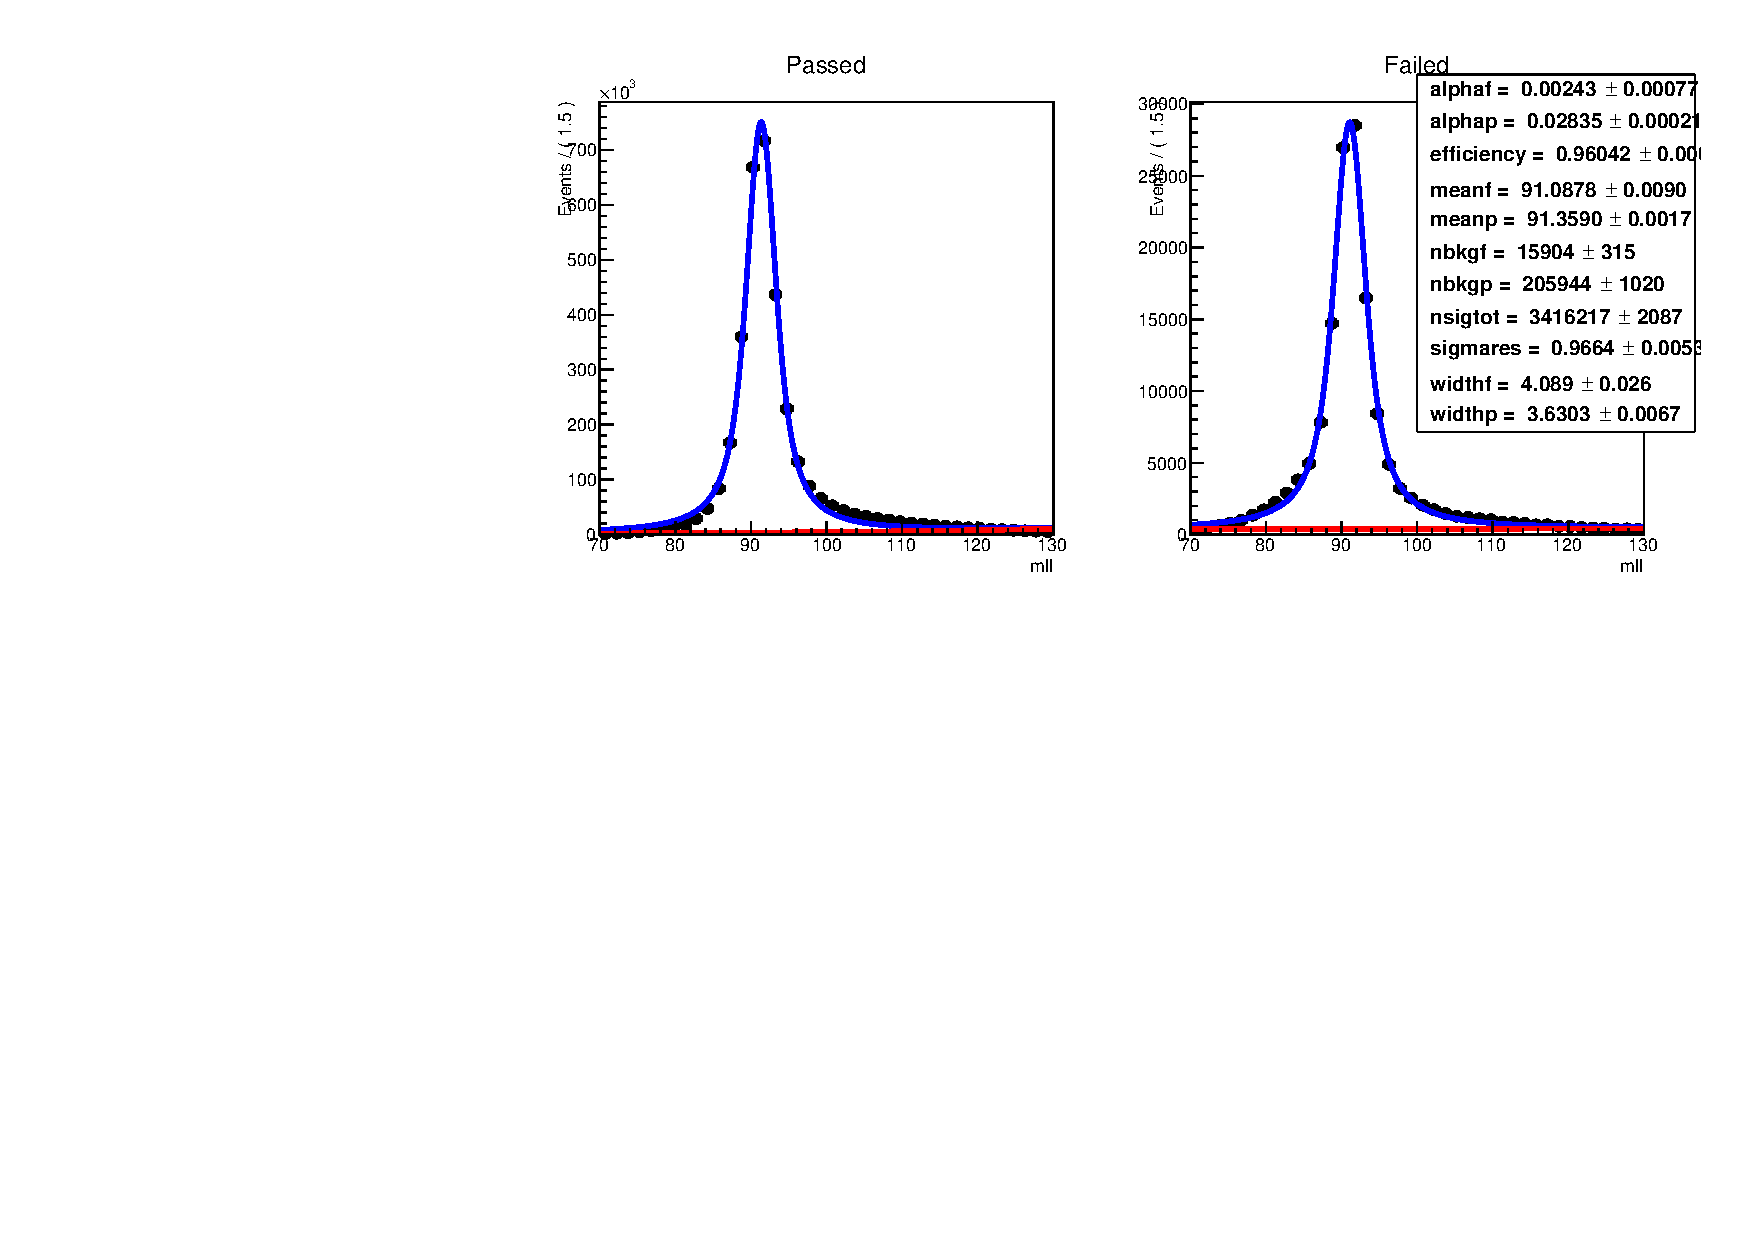
\includegraphics[width=0.9\textwidth]{figs/analysis/muonIsolationTight_mll_all_muonDefaultPtBins_pt50-60_Data}
\caption{Result of the tag-and-probe dimuon invariant mass fitting procedure to 
passing (left) and failing (right) probes for an example isolation efficiency 
measurement in data for muons with $50<\pt<60$~GeV. The blue (red) curves are 
the fitted signal (background) distributions. The fitted efficiency in this 
example is 96.0\%.}
\end{figure}

The efficiencies and corresponding data-to-simulation corrections are derived 
as a function of muon \pt and $\eta$. The identification efficiency is around 
97-99\% and the corresponding correction factors are in the range 0.97-0.99. 
The efficiency 
of the isolation requirement varies between 90-99\% and the correction factors 
are around 0.99-1. The trigger efficiency is measured to be approximately 90\%, 
with correction factors of about 0.98. 
In the \mmj control region, the trigger efficiency is higher, as the 
probability to trigger on at least one muon is $\approx 1-(1-0.9)(1-0.9) = 
99\%$.
The correction factors are then used to weight the simulated events in the muon 
control regions.
%need to describe how trigger SFs are applied to double muon CR.
%assumes indep? yes
% this is wrong (apply DATA effs):
%https://github.com/CMSRA1/AlphaTools/blob/v1.10.x/analysis/Producers/WeightSFLeptonEtaPtCRMuons.py#L153
% SF should be 1-(1-effD1)*(1-effD2) / 1-(1-effM1)*(1-effM2)

\subsection{Trigger}
Unlike the muon triggers, the signal region triggers are not emulated in the 
simulation. Instead of determining data-to-simulation correction factors, the 
trigger efficiencies measured in data as a function of \scalht and \mht using 
an electron reference sample (as described in Sec.~\ref{sec:analysis-trigger}) 
are themselves applied as corrections. As seen in 
Fig.~\ref{fig:trigger-eff}, these can be as low as 90\% at low \mht, but 
are close to unity for $\mht>300$~GeV.

\subsection{Jet energy scale}
TODO?
Lepton veto?

%\subsection{NLO precision of V+jets production}
\subsection{Theoretical calculation of V+jets production}
%2 plots?
%Electroweak corrections play an especially important role in the context of BSM
%searches, due to the presence of large EW Sudakov logarithms at the TeV scale
As mentioned in Sec.~\ref{sec:analysis-samples-mc}, the simulation samples for 
the vector boson production processes, namely \zj and \wj, are generated at 
leading order, as this allows a larger number of events to be simulated. 
The samples are corrected for missing higher orders as a function of the 
boson's transverse momentum. This is done by deriving NLO QCD correction 
factors using \textsc{Madgraph5}, and NLO electroweak correction factors from 
theoretical calculations~\cite{nlo,nlo}. The combined NLO QCD+EW corrections 
range from approximately 1.4 at a boson \pt of 200~GeV to 0.9 at 800~GeV, for 
both the \zj and \wj processes.
% see bosonptsystematics slides - bulk is boson pt 200, tail is 800

%https://arxiv.org/pdf/1511.08692.pdf
%https://arxiv.org/pdf/1412.5157.pdf

%Therefore, LO simulations for the Z + jets, W + jets, and g + jets processes 
%are corrected using pT-dependent NLO QCD K-factors derived using 
%%MADGRAPH5aMC@NLO. They are also corrected using pT-dependent higher-order 
%%electroweak (EW) corrections extracted from theoretical calculations

\subsection{Initial state radiation in \ttbar events}
% NO TOP PT REWEIGHTING! because for 8 TeV
\begin{comment}
https://twiki.cern.ch/twiki/bin/viewauth/CMS/SUSRecommendationsMoriond17
To improve on the MadGraph modeling of the multiplicity of additional jets from 
initial state radiation (ISR), Madgraph \ttbar Monte Carlo events are 
reweighted based on the number of ISR jets ($N_J^{ISR}$) so as to make the jet
multiplicity agree with data.  The same reweighting procedure is applied to 
SUSY Monte Carlo events.
The reweighting factors vary between 0.92 and 0.51 for $N_J^{ISR}$ between 1 
and 6. 
We take one half of the deviation from unity as the systematic uncertainty on 
these reweighting factors
\end{comment}
%% 
%%https://indico.cern.ch/event/592621/contributions/2398559/attachments/1383909/2105089/16-12-05_ana_manuelf_isr.pdf
%% require 2ℓ and exactly 2 b-tagged jets - remaining jets define ISR jet 
%%multiplicity and ISR pT

Simulated events of the \ttbar background process are weighted to improve the 
agreement with data of the multiplicity of jets from initial state radiation. 
The data-to-simulation correction factors are derived as a function of the 
number of ISR jets in an event, and take on values between 0.92 and 0.51 for an 
ISR multiplicity of 1 and 6, respectively.

\subsection{Cross-sections}
%correction to finite precision of xs calculation.
Although the dominant standard model background processes are normalised using 
the most accurate cross section calculations available (using NLO or NNLO 
precision), the finite perturbative order combined with the high \scalht and 
\met selections means that the overall simulated yields of the SM processes in 
the search regions are not in agreement with those in data.

% do fit instead of counting because have admixture of processes and not easy 
%to subtract backgrounds
Corrections to the cross sections of the dominant background processes, namely 
\zj, \wj and \ttbar, that are appropriate for the phase space covered by the 
search, are derived in a sideband of the \mj and \mmj control 
regions defined by a selection of $100<\mht<200$~GeV.
The two \mht sidebands are binned in \njet, \nb and \scalht identically to 
their control region counterparts.
%same (as similar as poss) phase space as analysis.
The procedure is done after all other corrections to the simulation samples 
have been applied.

%sideband instead of CR because need orthogonal samples (don't want to derive a 
%%%correction based on same data that will be used to correct MC in background 
%%%prediction).

%signal contam? doesn't affect predictions.
%depleted of signal.

%doesn't affect predictions but would inflate systs unnecessarily. 
%affects admixture? well if admixture is same in SR and CR then also cancels out
As the background composition in the signal and control regions is similar, 
these cross section corrections have a very small effect on the background 
estimations as they cancel out in the simulation-based transfer factor ratios 
(explained in 
Sec.~\ref{sec:analysis-estimation-njnbht}). However, this is not the case for 
some of the tests that are used to derived systematic uncertainties (which will 
be described in Sec.~\ref{sec:analysis-systematics-data}) and so the lack of 
corrections would unnecessarily inflate these uncertainties.

%Z,W,tt. (apply DY to Z).

In order to extract the cross section correction factors, a simultaneous binned 
maximum likelihood fit is performed over both \mht sideband regions, in which 
the three correction parameters (one for each of the \zj, \wj and \ttbar 
processes) are freely floating such that they modify the simulated yields to 
give the best agreement with those in data. The likelihood function is given by:
%rate parameters (lnU). same param in each bin.
%likelihood formula.
%actually lnU but doesn't really matter
\begin{equation}
\mathcal{L} = \mathcal{U}(f_{\mathrm W}) \mathcal{U}(f_{\mathrm Z}) 
\mathcal{U}(f_{\ttbar}) 
\prod_{b~(\mu+\mathrm{jets})} 
\mathcal{P}\left(f_{\mathrm W} \lambda_{\mathrm W}^b + 
f_{\ttbar} \lambda_{\ttbar}^b\right) \prod_{b~(\mu\mu+\mathrm{jets})} 
\mathcal{P}\left(f_{\mathrm 
Z} \lambda_{\mathrm Z}^b + f_{\ttbar} \lambda_{\ttbar}^b\right)
\end{equation}
where the $\lambda^b$'s are the number of background events in an \njnbht bin 
$b$ given by the simulation for a given standard model process, the $f$'s are 
the cross section correction factors, the $\mathcal{U}$'s define a uniform 
distribution for the correction parameters, and the $\mathcal{P}$'s define a 
Poisson distribution in each bin. 

The cross section correction factors for the \zj, \wj and \ttbar processes are 
mainly constrained, respectively, by the \mmj sideband, the \mj sideband, and a 
combination of the two sidebands. The values of the correction factors obtained 
from the fit are given in Tab.~\ref{tab:sideband-corrs}.
\begin{table}[h!]
%\footnotesize
\centering
\caption{Cross section correction factors for the three dominant standard model 
background processes, along with an indication of the most constraining 
sideband region for each process.}
\label{tab:sideband-corrs}
\begin{tabular}{ccc}
\hline
SM process & Sideband region & Correction factor \\
\hline
\zj    & \mmj      & $f_{\mathrm Z} = 0.91$ \\
\wj    & \mj       & $f_{\mathrm W} = 1.06$ \\
\ttbar & \mj, \mmj & $f_{\ttbar} = 0.93$ \\
\hline
\end{tabular}
\end{table}

%\subsection{Plus more?}
%NLO, pdf/scale.
%Signal (maybe later): nISR, gen met

\subsection{Statistical precision at large \nb}
%b-tag formula method
%1-2 pages.
%See Burton. AN Sec 4.4.
%Relevant but be brief.
%not really correction but rather improvement of stat precision at high nb.
%Purpose: reduce stat uncertainty of simulation in higher nb bins (where signal 
%can lie).
The following describes a method by which the statistical precision of the 
background simulation samples in the high \nb bins is improved. This is 
particularly useful for the $\nb \ge 3$ region, which is populated by standard 
model processes through the incorrect tagging of light flavour jets as b-jets, 
mainly \ttbar events in which the two b-jets from the top quarks are correctly 
tagged and an additional jet is mistagged. As the mistagging probability is 
quite small, the number of such events in simulation is limited. Reducing the 
statistical uncertainty on the expected standard model background in the high 
\nb region helps to improve the sensitivity of the search to SUSY and DM 
processes involving the production of multiple heavy quarks, as well as 
processes containing displaced jets, as will be seen in 
Chap.~\ref{chap:results}.
%Events from the \zj and \wj processes usually do not contain any b-jets. 
%Events from \ttbar typically contain two b-jets
%called the \nb \textit{formula method}

First, the b-tagging probabilities for bottom, charm and light flavour jets 
($\varepsilon_\mathrm b$, $\varepsilon_\mathrm c$, $\varepsilon_\mathrm l$) are 
computed in simulation in bins of (\nj, \scalht, \mht), after applying the \pt 
and $\eta$ dependent correction weights described in 
Sec.~\ref{sec:analysis-corrections-btagging}.
For a given number of jets $n_q^\mathrm{gen}$ of underlying flavour $q$ (as 
determined by generator-level information), the number of such jets that are 
b-tagged $n_q^\mathrm{tag}$ follows a binomial distribution with probability 
parameter $\varepsilon_q$, $P(n_q^\mathrm{tag}|n_q^\mathrm{gen}, 
\varepsilon_q)$. For an event containing a particular combination of 
underlying jet flavours ($n_\mathrm b^\mathrm{gen}$, $n_\mathrm 
c^\mathrm{gen}$, $n_\mathrm l^\mathrm{gen}$), the probability of observing a 
combination of b-tagged jets ($n_\mathrm b^\mathrm{tag}$, $n_\mathrm 
c^\mathrm{tag}$, $n_\mathrm l^\mathrm{tag}$) is given by the product:
\begin{equation}
P\left( n_\mathrm b^\mathrm{tag}, n_\mathrm c^\mathrm{tag}, n_\mathrm 
l^\mathrm{tag} | n_\mathrm b^\mathrm{gen}, n_\mathrm c^\mathrm{gen}, n_\mathrm 
l^\mathrm{gen} \right) = P\left(n_\mathrm b^\mathrm{tag}|n_\mathrm 
b^\mathrm{gen}, \varepsilon_\mathrm b\right) P\left(n_\mathrm 
c^\mathrm{tag}|n_\mathrm c^\mathrm{gen}, \varepsilon_\mathrm c\right) 
P\left(n_\mathrm l^\mathrm{tag}|n_\mathrm l^\mathrm{gen}, \varepsilon_\mathrm 
l\right) \, .
\end{equation}
If there are $N\left(n_\mathrm b^\mathrm{gen}, n_\mathrm 
c^\mathrm{gen}, n_\mathrm l^\mathrm{gen}\right)$ simulation events of a 
particular process with such 
combination of underlying jet flavour, the number of these events that result 
in a combination of b-tagged jets ($n_\mathrm b^\mathrm{tag}$, $n_\mathrm 
c^\mathrm{tag}$, $n_\mathrm l^\mathrm{tag}$) follows a binomial distribution 
with the above probability, with an expected value of:
\begin{equation}
E\left[N\left(n_\mathrm 
b^\mathrm{tag}, n_\mathrm c^\mathrm{tag}, n_\mathrm l^\mathrm{tag} | n_\mathrm 
b^\mathrm{gen}, n_\mathrm c^\mathrm{gen}, n_\mathrm l^\mathrm{gen}\right) 
\right] = N\left(n_\mathrm 
b^\mathrm{gen}, n_\mathrm c^\mathrm{gen}, n_\mathrm l^\mathrm{gen}\right) 
P\left( n_\mathrm b^\mathrm{tag}, n_\mathrm c^\mathrm{tag}, n_\mathrm 
l^\mathrm{tag} | n_\mathrm b^\mathrm{gen}, n_\mathrm c^\mathrm{gen}, n_\mathrm 
l^\mathrm{gen} \right) \, .
\end{equation}
The total expected number of events containing \nb b-tagged jets in a given 
(\njet, \scalht, \mht) bin is then the 
sum of this expected value over all combinations of underlying jet flavours 
that sum to \njet and all combinations of b-tagged jets that sum to \nb:
\begin{equation}
N(\nb) = \sum_{n_\mathrm b^\mathrm{gen} + n_\mathrm c^\mathrm{gen} + n_\mathrm 
l^\mathrm{gen} = \njet} ~ \sum_{n_\mathrm b^\mathrm{tag} + n_\mathrm 
c^\mathrm{tag} + n_\mathrm l^\mathrm{tag} = \nb} E\left[N\left(n_\mathrm 
b^\mathrm{tag}, n_\mathrm c^\mathrm{tag}, n_\mathrm l^\mathrm{tag} | n_\mathrm 
b^\mathrm{gen}, n_\mathrm c^\mathrm{gen}, n_\mathrm l^\mathrm{gen}\right) 
\right] \, .
\end{equation}

The strength of the method comes from a more effective utilisation of all 
simulated events.
%in calculating the expected number of events in each \nb bin. 
Each simulated event, rather than resulting in one particular ($n_\mathrm 
b^\mathrm{tag}$, $n_\mathrm c^\mathrm{tag}$, $n_\mathrm l^\mathrm{tag}$) 
realisation, contributes to the estimation of the yield in multiple \nb bins.
%eff uses info from all simulation events, and each event contributes to 
%multiple bins rather than just one particular realisation.
\textbf{The statistical uncertainties are found to be x times smaller than 
those 
obtained directly from the simulated events.. in nb 3, 4... TODO}
As a means of validation, it is checked that the yields estimated with this 
method are consistent with those obtained directly from simulation.

%Summarise in table/plot or one-two sentences how much the stat unc is reduced. 
%How much improves limits? Just refer to T1bbbb as T1qqqqLL 1 mm is very 
%similar.
%Formula systematics.

Throughout the remainder of the thesis, all simulation-based event yields are 
obtained via this method. Similarly, all references to simulated events assume 
the inclusion of all the corrections described in this section. 

\section{Estimation of electroweak background processes}
\label{sec:analysis-estimation-ewk}
%Predict normalisation using CRs (data-driven to reduce reliance on MC). 
%Use MHT templates from MC.
%ttw = W + ttbar + residual backgrounds, from now on refer collectively as W/tt
An accurate knowledge of the expected number of standard model background 
events is very important when searching for new physics. Relying on simulation, 
even after applying the corrections discussed in the previous section, would 
introduce a bias in the background estimation due to imperfect modelling. A 
data-driven approach is therefore utilised which combines simulated events and 
control region data to perform a more accurate estimation.

This section describes the methods of background estimation for the electroweak 
processes, which involves an estimation per \njnbht bin and another one for the 
\mht bins within each \njnbht bin. The estimation of the much smaller QCD 
background will be discussed in Sec.~\ref{sec:analysis-estimation-qcd}.

\subsection{The \njet, \nb and \scalht dimensions}
\label{sec:analysis-estimation-njnbht}
%1 page
The number of background events in each \njnbht bin is estimated using the muon 
control regions. As mentioned in 
Sec.~\ref{sec:analysis-eventselection-cr}~and~\ref{sec:analysis-binning}, these 
are chosen to be enriched in the background processes they are trying to 
estimate and are binned identically in \njnbht (with the exception of the \nb 
dimension in the \mmj sample). The \mmj control region is used to estimate the 
\znnj background, while the \mj control region is used to estimate the sum of 
the \wlj, \ttbar and residual backgrounds, which will be collectively labelled 
as \ttw.

The estimated number of events of a given background process in a particular 
\njnbht bin is related to the total number of events in the same bin of the 
corresponding control region in data $N_\mathrm{control}^\mathrm{data}\njnbht$ 
and simulation $N_\mathrm{control}^\mathrm{sim}\njnbht$ and the number of 
events of that background in the same bin of the signal region in simulation 
$N_\mathrm{signal}^\mathrm{sim}\njnbht$ by:
%For a given \njnbht bin, one can define a transfer factor,
\begin{equation}
\label{eqn:estimation}
\hat{N}_\mathrm{signal}\njnbht = 
\frac{N_\mathrm{signal}^\mathrm{sim}\njnbht}{N_\mathrm{control}^\mathrm{sim}\njnbht}
 N_\mathrm{control}^\mathrm{data}\njnbht \, .
\end{equation}
A special case of this formula applies for the \znnj process in the $\nb=1, 2, 
3$~and~$\ge4$ bins, which is estimated in each of these bins using the $\nb \ge 
1$ bin in the \mmj control region.
\textbf{TODO: nb validation.}

The extrapolation from the control region to the signal region is performed via 
the simulation-based ratio of yields in the above equation, referred to as a 
\textit{transfer factor}:
\begin{equation}
T\njnbht  = 
\frac{N_\mathrm{signal}^\mathrm{sim}\njnbht}{N_\mathrm{control}^\mathrm{sim}\njnbht}
 \, .
\end{equation}
The transfer factor can be viewed as a way of accounting for the different 
branching fraction, acceptance and identification efficiency of a given process 
between the signal and control region. For instance, the Z boson's branching 
ratio between neutrinos and muons is 9, and unlike the weakly interacting 
neutrinos, the muons are subject to acceptance and identification requirements. 
The transfer factor also accounts for the different kinematic selections, 
namely on \alphat and \bdphi, which are not used in the control regions.

\textbf{TODO give size of TFs? Put 2 plots here or in appendix. See comments 
and answers from Phil or whatevs.}

Equivalently, the estimation in Eq.~\ref{eqn:estimation} can also be viewed as 
a way of correcting the number of events obtained from the simulation according 
to the data-to-simulation discrepancy ratio in the control region bin:
\begin{equation}
\hat{N}_\mathrm{signal}\njnbht = 
\frac{N_\mathrm{control}^\mathrm{data}\njnbht}{N_\mathrm{control}^\mathrm{sim}\njnbht}
N_\mathrm{signal}^\mathrm{sim}\njnbht \, .
\end{equation}
This highlights the importance of having similar kinematic requirements and 
background compositions, as well as a similar binning scheme, in the control 
and signal regions, as the discrepancy between data and simulation in a given 
bin of the control region is likely to be similar to that in the corresponding 
bin in the signal region.
% see njet discrepancy argument in adam

The transfer factors, and therefore the background estimations, are robust 
against many sources of systematic effects relating to kinematic mismodelling 
and theoretical uncertainties, 
as these cancel out in the transfer factor ratio to a large extent.
%This is because the background estimations are 
%performed between equivalent \njnbht bins of the signal and control regions, 
%which contain a similar background composition 
%and so cancel out in the transfer factor ratio to a large extent.
Several sources of systematic uncertainty are nevertheless accounted for in the 
estimated backgrounds, as will be discussed in 
Sec.~\ref{sec:analysis-systematics}.
%syst effects cancel in TF. because similar events in SR and CR.

\subsection{The \mht dimension}
\label{sec:analysis-estimation-mht}
%2 pages

If it helps (to give intro), see AN and matt's mht categorisation sections.

Take templates because don't want to bin CRs too finely (lose statistical power 
- curse of dimensionality).
CRs not binned in mht.

Validation: Check data MC ratio is flat in CRs. Assign syst as described later 
in Sec X.

\section{Estimation of QCD background processes}
\label{sec:analysis-estimation-qcd}
2 pages

Method.

Validation.

Plot of estimated yields per bin.

\section{Systematic uncertainties on background estimation}
\label{sec:analysis-systematics}.

These are explained below and also summarised, with representative magnitudes, 
in the big summary table of systs.

(don't know where to put it)
Show nb extrapolation validation (AN) or just summarise briefly in couple of 
sentences (similar to MHT validation).

Formula systematics.

\subsection{MC-based}
\label{sec:analysis-systematics-mc}
3-4 pages (maybe 2 pages just of plots).

Known theoretical and experimental uncertainties.
Largely cancel out in the TF ratio.

Refer to Section of corrections to simulation. These are the associated 
uncertainties.

Pileup, JEC, b-tagging, lepton, photon, trigger, top pt, W/tt, NLO, ttbar nISR.

Example 2D plots of variations in the bins.

Efficiencies then applied to simulation as a correction to match data and a 
systematic uncertainty is assigned based on differences between electron and 
muon reference trigger, see Sections corrections and systematics.

boson pt NLO syst 100\% of correction.

\subsection{Closure tests}
\label{sec:analysis-systematics-data}
2-3 pages.

Probe additional sources of systematics.

Define method.

Go through each test (there's not many now) and describe what it's probing: 
extrapolation in alphat and bdphi, W polarisation, SITV.

Closure plots.

\subsection{MHT templates}
2 pages. See Matt and old ANs.

Derivation of uncertainties. Vs njet and ht.

Plot illustrating size of uncertainty in each bin.
